\documentclass[twoside]{book}

% Packages required by doxygen
\usepackage{fixltx2e}
\usepackage{calc}
\usepackage{doxygen}
\usepackage[export]{adjustbox} % also loads graphicx
\usepackage{graphicx}
\usepackage[utf8]{inputenc}
\usepackage{makeidx}
\usepackage{multicol}
\usepackage{multirow}
\PassOptionsToPackage{warn}{textcomp}
\usepackage{textcomp}
\usepackage[nointegrals]{wasysym}
\usepackage[table]{xcolor}

% Font selection
\usepackage[T1]{fontenc}
\usepackage[scaled=.90]{helvet}
\usepackage{courier}
\usepackage{amssymb}
\usepackage{sectsty}
\renewcommand{\familydefault}{\sfdefault}
\allsectionsfont{%
  \fontseries{bc}\selectfont%
  \color{darkgray}%
}
\renewcommand{\DoxyLabelFont}{%
  \fontseries{bc}\selectfont%
  \color{darkgray}%
}
\newcommand{\+}{\discretionary{\mbox{\scriptsize$\hookleftarrow$}}{}{}}

% Page & text layout
\usepackage{geometry}
\geometry{%
  a4paper,%
  top=2.5cm,%
  bottom=2.5cm,%
  left=2.5cm,%
  right=2.5cm%
}
\tolerance=750
\hfuzz=15pt
\hbadness=750
\setlength{\emergencystretch}{15pt}
\setlength{\parindent}{0cm}
\setlength{\parskip}{3ex plus 2ex minus 2ex}
\makeatletter
\renewcommand{\paragraph}{%
  \@startsection{paragraph}{4}{0ex}{-1.0ex}{1.0ex}{%
    \normalfont\normalsize\bfseries\SS@parafont%
  }%
}
\renewcommand{\subparagraph}{%
  \@startsection{subparagraph}{5}{0ex}{-1.0ex}{1.0ex}{%
    \normalfont\normalsize\bfseries\SS@subparafont%
  }%
}
\makeatother

% Headers & footers
\usepackage{fancyhdr}
\pagestyle{fancyplain}
\fancyhead[LE]{\fancyplain{}{\bfseries\thepage}}
\fancyhead[CE]{\fancyplain{}{}}
\fancyhead[RE]{\fancyplain{}{\bfseries\leftmark}}
\fancyhead[LO]{\fancyplain{}{\bfseries\rightmark}}
\fancyhead[CO]{\fancyplain{}{}}
\fancyhead[RO]{\fancyplain{}{\bfseries\thepage}}
\fancyfoot[LE]{\fancyplain{}{}}
\fancyfoot[CE]{\fancyplain{}{}}
\fancyfoot[RE]{\fancyplain{}{\bfseries\scriptsize Generated by Doxygen }}
\fancyfoot[LO]{\fancyplain{}{\bfseries\scriptsize Generated by Doxygen }}
\fancyfoot[CO]{\fancyplain{}{}}
\fancyfoot[RO]{\fancyplain{}{}}
\renewcommand{\footrulewidth}{0.4pt}
\renewcommand{\chaptermark}[1]{%
  \markboth{#1}{}%
}
\renewcommand{\sectionmark}[1]{%
  \markright{\thesection\ #1}%
}

% Indices & bibliography
\usepackage{natbib}
\usepackage[titles]{tocloft}
\setcounter{tocdepth}{3}
\setcounter{secnumdepth}{5}
\makeindex

% Hyperlinks (required, but should be loaded last)
\usepackage{ifpdf}
\ifpdf
  \usepackage[pdftex,pagebackref=true]{hyperref}
\else
  \usepackage[ps2pdf,pagebackref=true]{hyperref}
\fi
\hypersetup{%
  colorlinks=true,%
  linkcolor=blue,%
  citecolor=blue,%
  unicode%
}

% Custom commands
\newcommand{\clearemptydoublepage}{%
  \newpage{\pagestyle{empty}\cleardoublepage}%
}

\usepackage{caption}
\captionsetup{labelsep=space,justification=centering,font={bf},singlelinecheck=off,skip=4pt,position=top}

%===== C O N T E N T S =====

\begin{document}

% Titlepage & ToC
\hypersetup{pageanchor=false,
             bookmarksnumbered=true,
             pdfencoding=unicode
            }
\pagenumbering{alph}
\begin{titlepage}
\vspace*{7cm}
\begin{center}%
{\Large Road\+Gen\+L\+Systems \\[1ex]\large 1.\+0 }\\
\vspace*{1cm}
{\large Generated by Doxygen 1.8.12}\\
\end{center}
\end{titlepage}
\clearemptydoublepage
\pagenumbering{roman}
\tableofcontents
\clearemptydoublepage
\pagenumbering{arabic}
\hypersetup{pageanchor=true}

%--- Begin generated contents ---
\chapter{Road generation based on L-\/\+Systems}
\label{index}\hypertarget{index}{}\hypertarget{index_intro_sec}{}\section{Introduction}\label{index_intro_sec}
The road generator was created as part of a bachelor thesis at the T\+U-\/\+Graz. Its main goal was to create a visually appealing road system, which will later be used in combinations with shape grammars (procedural modeling) to generate a complete city from scratch.

The system has to be able to generate a visually appealing city map, containing rivers as well as green-\/spaces and parking lots next to the lots for the city-\/blocks itself. The generated result is configurable by the user in an easy way, so that a lot of different street patterns can be computed without greater foreknowledge. This is done by providing the input files to the programm at creation (See \char`\"{}all\+\_\+parm.\+txt\char`\"{} as well as \char`\"{}all\+\_\+points.\+txt\char`\"{})

To create unique looking maps with an easily understandable underlying model, L-\/\+Systems were used. The L-\/\+System used a linked-\/list of non-\/terminal symbols, which were imple-\/ mented using different classes for each symbol. Instances of the classes will replace them-\/ selves in the list, until every instance has terminated. Non-\/terminal symbols are\+:


\begin{DoxyItemize}
\item \hyperlink{class_n_t_start}{N\+T\+Start}
\item \hyperlink{class_n_t_highway}{N\+T\+Highway}
\item \hyperlink{class_n_t_highway_segment}{N\+T\+Highway\+Segment}
\item \hyperlink{class_n_t_street}{N\+T\+Street}
\end{DoxyItemize}

Before creating any of the roads, rivers are created. The amount of rivers used in the map can be configured by the user. Rivers grow from one (random) side of the map to the other. After doing so, the algorithm first creates a set of highways, which serve as anchor points for the generation of smaller roads. During creation, two set of rules are used in order to create visually appealing networks, which can be split in global and local rules.\hypertarget{index_Global}{}\subsection{Global}\label{index_Global}
The global rules only apply to the creation of highway segments. These major traffic aortae are used as branching point for smaller street segments. In order to gain some visual control over the network generation, the user is able to place n-\/start points, from which highway segments will start growing towards m-\/target points. Each start point is represented by one member of the \hyperlink{class_n_t_highway}{N\+T\+Highway} class, which will create m-\/\+Highway\+Segments, growing towards every of the goal points (segments terminate at collision or if the goal is reached). Every time a highway segment replaces itself with a new segment, a direct segment towards the goal is calculated (fixed length). After doing so a random offset is added, in order to make the creation look less linear.



Another characteristic of the highways is, that they are able to create bridges spanning rivers. Before a highway segment grows towards the goal, it is first checked if any river would inter-\/ fere with the new segment and if so where. The algorithm then tries to get the other riverbank by extruding the conflict segment. If the two points could be acquired, a bridge can be con-\/ structed between them. The old segment is only produced up to the first conflict point, while on the other side of the river a new highway-\/segment is created and inserted into the list.

After the last highway has finished (either by reaching the goal or by intersecting another highway segment), branching of the streets starts. Not waiting for the highways to terminate might otherwise lead to streets getting in the way of new highways, which would stop them mid-\/creation.\hypertarget{index_Local}{}\subsection{Local}\label{index_Local}
Every time a highway segment grows outwards, it has a (user selected) possibility to create a new street branch (branching-\/probability). Streets grow towards random locations, only keeping the angle relative to the previous street segment in mind (do not want too steep angles, should look natural). If the new segment is calculated, a check for intersections is necessary (when found, terminate the segment at the collision).\hypertarget{index_Lots}{}\subsection{Lots}\label{index_Lots}
The road network keeps growing until every element in the list has terminated. The created segments are stored in corresponding containers. Until now only segments were created, but as the lot creation algorithm needs polygons to work with, they had to be calculated by using the given segments as well as {\bfseries C\+P\+S\+Gs} {\bfseries 2\+D-\/\+Arrangement} functionality.



By doing so polygons were created without any margin between them for the streets. This problem was solved by using the {\bfseries C\+L\+I\+P\+P\+E\+R-\/\+Library} to shrink the given polygons evenly.

~\newline
 \hypertarget{index_install_sec}{}\section{Installation}\label{index_install_sec}
\hypertarget{index_windows}{}\subsection{Windows}\label{index_windows}

\begin{DoxyItemize}
\item Download source from \href{https://github.com/LGrege/RoadNetworkGenerator}{\tt https\+://github.\+com/\+L\+Grege/\+Road\+Network\+Generator}
\item Install C\+M\+A\+KE from \href{https://cmake.org/download/}{\tt https\+://cmake.\+org/download/}
\item Follow the instructions under \href{http://www.cgal.org/download/windows.html}{\tt http\+://www.\+cgal.\+org/download/windows.\+html} to install C\+G\+AL
\item Use C\+M\+A\+KE to generate the Visual Studio project ~\newline
 
\item Open the project in visual studio and build it using the release settings ~\newline
 
\item After building is done, a main.\+exe file is created under the Release folder
\end{DoxyItemize}\hypertarget{index_usage_sec}{}\section{Usage}\label{index_usage_sec}
The previously created executable expects two files as input, which have to be placed in the same directory as the file. These files are a config file as well as a input file (both .txt).\hypertarget{index_config_file}{}\subsection{Config}\label{index_config_file}
The name of the config file has to be \char`\"{}all\+\_\+parms.\+txt\char`\"{}. Example config file\+:


\begin{DoxyCode}
DAY-1
BP-87
LP-33
RC-1
MS-8000
DIM-600x800
\end{DoxyCode}


The input values are\+:
\begin{DoxyItemize}
\item D\+AY -\/$>$ Sets a flag in the output files later used for building creation (not relevant for road creation)
\item BP -\/$>$ Branch Probability, defines probability that street segment creates new branch. If higher, road network gets finer (lesser big lots)
\item LP -\/$>$ Lighting Probability, based on this parameter the amount of lights placed on the map can be manipulated
\item RC -\/$>$ River Count, Number of rivers to be created
\item MS -\/$>$ Max Segment, Maximum number of segments after which creation terminates. If dimension is increased, this value has to be increased also.
\item D\+IM -\/$>$ Dimension of the Map
\end{DoxyItemize}

Inputs that are not set are set by default with the values shown in the above configuration.\hypertarget{index_input_file}{}\subsection{Input}\label{index_input_file}
The name of the input file has to be \char`\"{}all\+\_\+points.\+txt\char`\"{} and has to look as follows\+:


\begin{DoxyCode}
L-87-124
R-312-115
L-639-99
R-45-435
L-393-359
R-704-357
\end{DoxyCode}


The \char`\"{}\+L\char`\"{}-\/\+Points define start points from which the road highways start to grow towards the \char`\"{}\+R\char`\"{}-\/\+Points (End points). An arbitrary amount of start and end points can be created, shaping the way the road network will look.\hypertarget{index_generated_output}{}\section{Output}\label{index_generated_output}
The resulting lots as well as rivers are exported to a generated folder, containing subfolders for the corresponding entities. Depending on the type of object exported, they are either J\+S\+ON or .txt files (later needed for another project).

Also two postscript files are created in the root directory, displaying the road network itself (\char`\"{}out.\+ps\char`\"{}) as well as the generated lot-\/polygons of the city blocks (\char`\"{}poly.\+ps\char`\"{})

~\newline
 \hypertarget{index_ack_sec}{}\section{Acknowledgments}\label{index_ack_sec}

\begin{DoxyItemize}
\item Clipper library was used for shrinking the polygons \href{http://www.angusj.com/delphi/clipper.php}{\tt http\+://www.\+angusj.\+com/delphi/clipper.\+php}
\item C\+G\+AL was used throughout the whole project \href{http://www.cgal.org/}{\tt http\+://www.\+cgal.\+org/} 
\end{DoxyItemize}
\chapter{Hierarchical Index}
\section{Class Hierarchy}
This inheritance list is sorted roughly, but not completely, alphabetically\+:\begin{DoxyCompactList}
\item \contentsline{section}{Clipper\+Lib\+:\+:Clipper\+Base}{\pageref{class_clipper_lib_1_1_clipper_base}}{}
\begin{DoxyCompactList}
\item \contentsline{section}{Clipper\+Lib\+:\+:Clipper}{\pageref{class_clipper_lib_1_1_clipper}}{}
\end{DoxyCompactList}
\item \contentsline{section}{Clipper\+Lib\+:\+:Clipper\+Offset}{\pageref{class_clipper_lib_1_1_clipper_offset}}{}
\item \contentsline{section}{Clipper\+Lib\+:\+:Double\+Point}{\pageref{struct_clipper_lib_1_1_double_point}}{}
\item \contentsline{section}{Entity\+Container}{\pageref{class_entity_container}}{}
\item exception\begin{DoxyCompactList}
\item \contentsline{section}{Clipper\+Lib\+:\+:clipper\+Exception}{\pageref{class_clipper_lib_1_1clipper_exception}}{}
\end{DoxyCompactList}
\item \contentsline{section}{I\+Interpretable}{\pageref{class_i_interpretable}}{}
\begin{DoxyCompactList}
\item \contentsline{section}{Post\+Script\+Int\+Writer}{\pageref{class_post_script_int_writer}}{}
\end{DoxyCompactList}
\item \contentsline{section}{Clipper\+Lib\+:\+:Int128}{\pageref{class_clipper_lib_1_1_int128}}{}
\item \contentsline{section}{Clipper\+Lib\+:\+:Intersect\+Node}{\pageref{struct_clipper_lib_1_1_intersect_node}}{}
\item \contentsline{section}{Clipper\+Lib\+:\+:Int\+Point}{\pageref{struct_clipper_lib_1_1_int_point}}{}
\item \contentsline{section}{Clipper\+Lib\+:\+:Int\+Rect}{\pageref{struct_clipper_lib_1_1_int_rect}}{}
\item \contentsline{section}{Clipper\+Lib\+:\+:Join}{\pageref{struct_clipper_lib_1_1_join}}{}
\item \contentsline{section}{J\+S\+O\+N\+Generator}{\pageref{class_j_s_o_n_generator}}{}
\item \contentsline{section}{L\+Generator}{\pageref{class_l_generator}}{}
\item \contentsline{section}{Lighting\+Generator}{\pageref{class_lighting_generator}}{}
\item \contentsline{section}{Clipper\+Lib\+:\+:Local\+Minimum}{\pageref{struct_clipper_lib_1_1_local_minimum}}{}
\item \contentsline{section}{Clipper\+Lib\+:\+:Loc\+Min\+Sorter}{\pageref{struct_clipper_lib_1_1_loc_min_sorter}}{}
\item \contentsline{section}{Non\+Terminal\+Symbol}{\pageref{class_non_terminal_symbol}}{}
\begin{DoxyCompactList}
\item \contentsline{section}{N\+T\+Highway}{\pageref{class_n_t_highway}}{}
\item \contentsline{section}{N\+T\+Highway\+Segment}{\pageref{class_n_t_highway_segment}}{}
\item \contentsline{section}{N\+T\+Start}{\pageref{class_n_t_start}}{}
\item \contentsline{section}{N\+T\+Street}{\pageref{class_n_t_street}}{}
\end{DoxyCompactList}
\item \contentsline{section}{Clipper\+Lib\+:\+:Out\+Pt}{\pageref{struct_clipper_lib_1_1_out_pt}}{}
\item \contentsline{section}{Clipper\+Lib\+:\+:Out\+Rec}{\pageref{struct_clipper_lib_1_1_out_rec}}{}
\item \contentsline{section}{Clipper\+Lib\+:\+:Poly\+Node}{\pageref{class_clipper_lib_1_1_poly_node}}{}
\begin{DoxyCompactList}
\item \contentsline{section}{Clipper\+Lib\+:\+:Poly\+Tree}{\pageref{class_clipper_lib_1_1_poly_tree}}{}
\end{DoxyCompactList}
\item \contentsline{section}{Clipper\+Lib\+:\+:T\+Edge}{\pageref{struct_clipper_lib_1_1_t_edge}}{}
\item \contentsline{section}{Tree\+Generator}{\pageref{class_tree_generator}}{}
\end{DoxyCompactList}

\chapter{Class Index}
\section{Class List}
Here are the classes, structs, unions and interfaces with brief descriptions\+:\begin{DoxyCompactList}
\item\contentsline{section}{\hyperlink{class_clipper_lib_1_1_clipper}{Clipper\+Lib\+::\+Clipper} }{\pageref{class_clipper_lib_1_1_clipper}}{}
\item\contentsline{section}{\hyperlink{class_clipper_lib_1_1_clipper_base}{Clipper\+Lib\+::\+Clipper\+Base} }{\pageref{class_clipper_lib_1_1_clipper_base}}{}
\item\contentsline{section}{\hyperlink{class_clipper_lib_1_1clipper_exception}{Clipper\+Lib\+::clipper\+Exception} }{\pageref{class_clipper_lib_1_1clipper_exception}}{}
\item\contentsline{section}{\hyperlink{class_clipper_lib_1_1_clipper_offset}{Clipper\+Lib\+::\+Clipper\+Offset} }{\pageref{class_clipper_lib_1_1_clipper_offset}}{}
\item\contentsline{section}{\hyperlink{struct_clipper_lib_1_1_double_point}{Clipper\+Lib\+::\+Double\+Point} }{\pageref{struct_clipper_lib_1_1_double_point}}{}
\item\contentsline{section}{\hyperlink{class_entity_container}{Entity\+Container} \\*Singleton Container class used by all \hyperlink{class_non_terminal_symbol}{Non\+Terminal\+Symbol} classes }{\pageref{class_entity_container}}{}
\item\contentsline{section}{\hyperlink{class_i_interpretable}{I\+Interpretable} \\*Interface declares interpretors for the gotten results }{\pageref{class_i_interpretable}}{}
\item\contentsline{section}{\hyperlink{class_clipper_lib_1_1_int128}{Clipper\+Lib\+::\+Int128} }{\pageref{class_clipper_lib_1_1_int128}}{}
\item\contentsline{section}{\hyperlink{struct_clipper_lib_1_1_intersect_node}{Clipper\+Lib\+::\+Intersect\+Node} }{\pageref{struct_clipper_lib_1_1_intersect_node}}{}
\item\contentsline{section}{\hyperlink{struct_clipper_lib_1_1_int_point}{Clipper\+Lib\+::\+Int\+Point} }{\pageref{struct_clipper_lib_1_1_int_point}}{}
\item\contentsline{section}{\hyperlink{struct_clipper_lib_1_1_int_rect}{Clipper\+Lib\+::\+Int\+Rect} }{\pageref{struct_clipper_lib_1_1_int_rect}}{}
\item\contentsline{section}{\hyperlink{struct_clipper_lib_1_1_join}{Clipper\+Lib\+::\+Join} }{\pageref{struct_clipper_lib_1_1_join}}{}
\item\contentsline{section}{\hyperlink{class_j_s_o_n_generator}{J\+S\+O\+N\+Generator} \\*Static class used to generate Polygons from the line-\/segments gotten by the L-\/\+System and write them to a J\+S\+ON / .txt -\/\+Files }{\pageref{class_j_s_o_n_generator}}{}
\item\contentsline{section}{\hyperlink{class_l_generator}{L\+Generator} \\*\hyperlink{class_l_generator}{L\+Generator} class for creating and managing used L-\/\+System }{\pageref{class_l_generator}}{}
\item\contentsline{section}{\hyperlink{class_lighting_generator}{Lighting\+Generator} \\*Used for placing Lights around the city. Different patterns for the lighting can be chosen here }{\pageref{class_lighting_generator}}{}
\item\contentsline{section}{\hyperlink{struct_clipper_lib_1_1_local_minimum}{Clipper\+Lib\+::\+Local\+Minimum} }{\pageref{struct_clipper_lib_1_1_local_minimum}}{}
\item\contentsline{section}{\hyperlink{struct_clipper_lib_1_1_loc_min_sorter}{Clipper\+Lib\+::\+Loc\+Min\+Sorter} }{\pageref{struct_clipper_lib_1_1_loc_min_sorter}}{}
\item\contentsline{section}{\hyperlink{class_non_terminal_symbol}{Non\+Terminal\+Symbol} \\*Parent class for all non-\/terminal members }{\pageref{class_non_terminal_symbol}}{}
\item\contentsline{section}{\hyperlink{class_n_t_highway}{N\+T\+Highway} \\*Start for the highway creation }{\pageref{class_n_t_highway}}{}
\item\contentsline{section}{\hyperlink{class_n_t_highway_segment}{N\+T\+Highway\+Segment} \\*Smallest unit of highway }{\pageref{class_n_t_highway_segment}}{}
\item\contentsline{section}{\hyperlink{class_n_t_start}{N\+T\+Start} \\*Start point of the overall creation }{\pageref{class_n_t_start}}{}
\item\contentsline{section}{\hyperlink{class_n_t_street}{N\+T\+Street} \\*Smalles unit of street }{\pageref{class_n_t_street}}{}
\item\contentsline{section}{\hyperlink{struct_clipper_lib_1_1_out_pt}{Clipper\+Lib\+::\+Out\+Pt} }{\pageref{struct_clipper_lib_1_1_out_pt}}{}
\item\contentsline{section}{\hyperlink{struct_clipper_lib_1_1_out_rec}{Clipper\+Lib\+::\+Out\+Rec} }{\pageref{struct_clipper_lib_1_1_out_rec}}{}
\item\contentsline{section}{\hyperlink{class_clipper_lib_1_1_poly_node}{Clipper\+Lib\+::\+Poly\+Node} }{\pageref{class_clipper_lib_1_1_poly_node}}{}
\item\contentsline{section}{\hyperlink{class_clipper_lib_1_1_poly_tree}{Clipper\+Lib\+::\+Poly\+Tree} }{\pageref{class_clipper_lib_1_1_poly_tree}}{}
\item\contentsline{section}{\hyperlink{class_post_script_int_writer}{Post\+Script\+Int\+Writer} \\*Generates Output (.pst File) from generated information }{\pageref{class_post_script_int_writer}}{}
\item\contentsline{section}{\hyperlink{struct_clipper_lib_1_1_t_edge}{Clipper\+Lib\+::\+T\+Edge} }{\pageref{struct_clipper_lib_1_1_t_edge}}{}
\item\contentsline{section}{\hyperlink{class_tree_generator}{Tree\+Generator} \\*Generates the trees (Placement in park) }{\pageref{class_tree_generator}}{}
\end{DoxyCompactList}

\chapter{Class Documentation}
\hypertarget{class_clipper_lib_1_1_clipper}{}\section{Clipper\+Lib\+:\+:Clipper Class Reference}
\label{class_clipper_lib_1_1_clipper}\index{Clipper\+Lib\+::\+Clipper@{Clipper\+Lib\+::\+Clipper}}
Inheritance diagram for Clipper\+Lib\+:\+:Clipper\+:\begin{figure}[H]
\begin{center}
\leavevmode
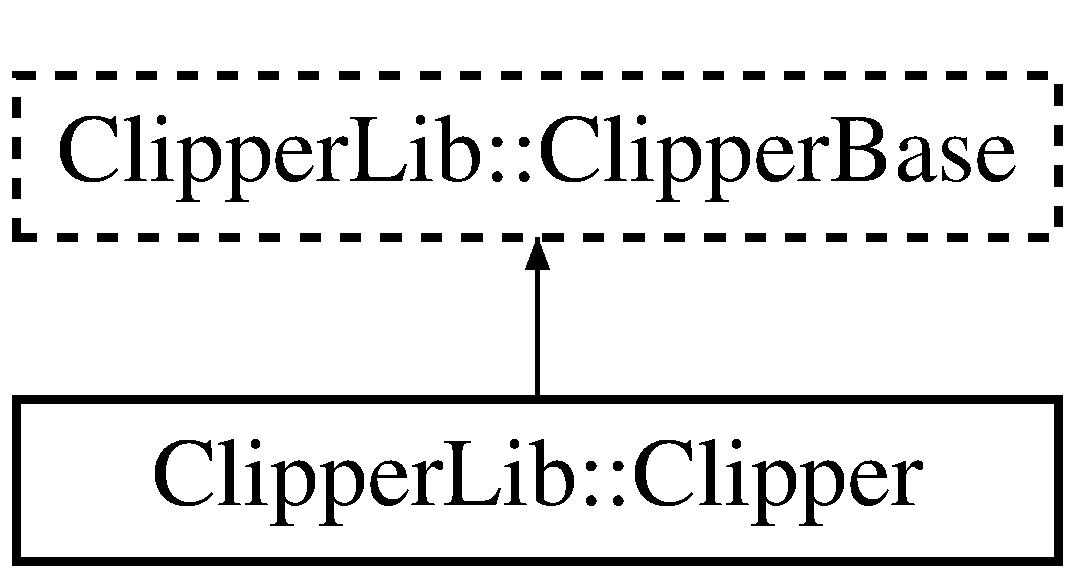
\includegraphics[height=2.000000cm]{class_clipper_lib_1_1_clipper}
\end{center}
\end{figure}
\subsection*{Public Member Functions}
\begin{DoxyCompactItemize}
\item 
\hypertarget{class_clipper_lib_1_1_clipper_adceb8536f6a80e8f115213dba9208427}{}\label{class_clipper_lib_1_1_clipper_adceb8536f6a80e8f115213dba9208427} 
{\bfseries Clipper} (int init\+Options=0)
\item 
\hypertarget{class_clipper_lib_1_1_clipper_a06da196a4b4151edd2e5426ed48744cf}{}\label{class_clipper_lib_1_1_clipper_a06da196a4b4151edd2e5426ed48744cf} 
bool {\bfseries Execute} (Clip\+Type clip\+Type, Paths \&solution, Poly\+Fill\+Type subj\+Fill\+Type=pft\+Even\+Odd, Poly\+Fill\+Type clip\+Fill\+Type=pft\+Even\+Odd)
\item 
\hypertarget{class_clipper_lib_1_1_clipper_aceb19a1e5a5c9e31067f4d1177793403}{}\label{class_clipper_lib_1_1_clipper_aceb19a1e5a5c9e31067f4d1177793403} 
bool {\bfseries Execute} (Clip\+Type clip\+Type, \hyperlink{class_clipper_lib_1_1_poly_tree}{Poly\+Tree} \&polytree, Poly\+Fill\+Type subj\+Fill\+Type=pft\+Even\+Odd, Poly\+Fill\+Type clip\+Fill\+Type=pft\+Even\+Odd)
\item 
\hypertarget{class_clipper_lib_1_1_clipper_ad556ba9961f498de02d55dc95bc5a889}{}\label{class_clipper_lib_1_1_clipper_ad556ba9961f498de02d55dc95bc5a889} 
bool {\bfseries Reverse\+Solution} ()
\item 
\hypertarget{class_clipper_lib_1_1_clipper_a44afc0c82a1d2607829b5fd21f7644ef}{}\label{class_clipper_lib_1_1_clipper_a44afc0c82a1d2607829b5fd21f7644ef} 
void {\bfseries Reverse\+Solution} (bool value)
\item 
\hypertarget{class_clipper_lib_1_1_clipper_a50eb4c514466ed37fd365769e0bcf67b}{}\label{class_clipper_lib_1_1_clipper_a50eb4c514466ed37fd365769e0bcf67b} 
bool {\bfseries Strictly\+Simple} ()
\item 
\hypertarget{class_clipper_lib_1_1_clipper_a85aa82d75e0d7d1f380d2e96231d6aa3}{}\label{class_clipper_lib_1_1_clipper_a85aa82d75e0d7d1f380d2e96231d6aa3} 
void {\bfseries Strictly\+Simple} (bool value)
\end{DoxyCompactItemize}
\subsection*{Protected Member Functions}
\begin{DoxyCompactItemize}
\item 
\hypertarget{class_clipper_lib_1_1_clipper_a14c704b062e8a079e34a8ce40838861e}{}\label{class_clipper_lib_1_1_clipper_a14c704b062e8a079e34a8ce40838861e} 
void {\bfseries Reset} ()
\item 
\hypertarget{class_clipper_lib_1_1_clipper_a3e8757e5f8a6ffcb7fd0f9630fde02d3}{}\label{class_clipper_lib_1_1_clipper_a3e8757e5f8a6ffcb7fd0f9630fde02d3} 
virtual bool {\bfseries Execute\+Internal} ()
\end{DoxyCompactItemize}
\subsection*{Additional Inherited Members}


The documentation for this class was generated from the following files\+:\begin{DoxyCompactItemize}
\item 
C\+:/\+Users/lukas/\+Desktop/\+Road\+Gen\+L\+Systems/Clipper.\+h\item 
C\+:/\+Users/lukas/\+Desktop/\+Road\+Gen\+L\+Systems/Clipper.\+cpp\end{DoxyCompactItemize}

\hypertarget{class_clipper_lib_1_1_clipper_base}{}\section{Clipper\+Lib\+:\+:Clipper\+Base Class Reference}
\label{class_clipper_lib_1_1_clipper_base}\index{Clipper\+Lib\+::\+Clipper\+Base@{Clipper\+Lib\+::\+Clipper\+Base}}
Inheritance diagram for Clipper\+Lib\+:\+:Clipper\+Base\+:\begin{figure}[H]
\begin{center}
\leavevmode
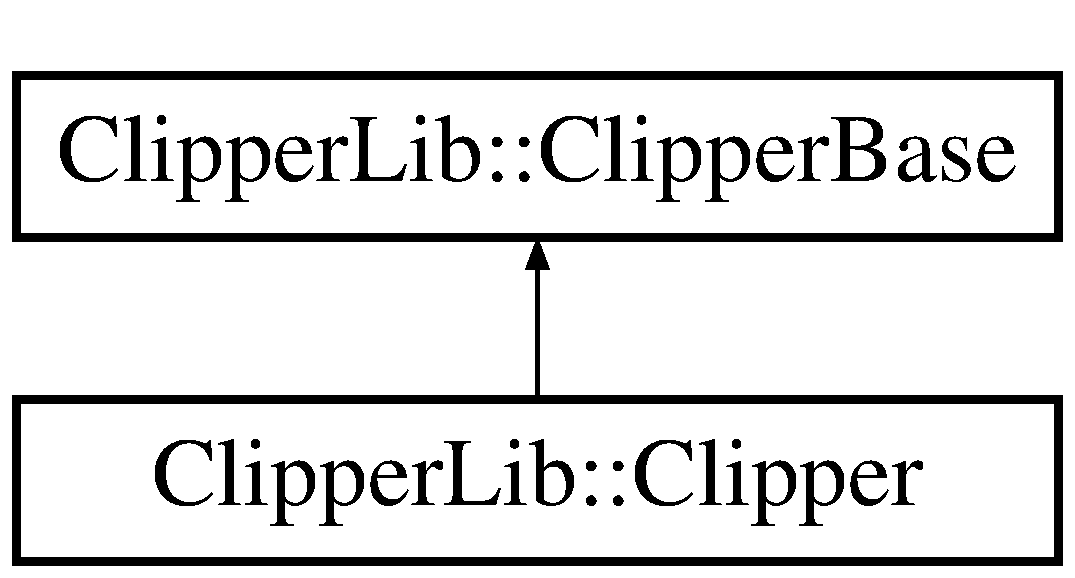
\includegraphics[height=2.000000cm]{class_clipper_lib_1_1_clipper_base}
\end{center}
\end{figure}
\subsection*{Public Member Functions}
\begin{DoxyCompactItemize}
\item 
\hypertarget{class_clipper_lib_1_1_clipper_base_a7545ac6e146894dc8416887eadd01dba}{}\label{class_clipper_lib_1_1_clipper_base_a7545ac6e146894dc8416887eadd01dba} 
bool {\bfseries Add\+Path} (const Path \&pg, Poly\+Type Poly\+Typ, bool Closed)
\item 
\hypertarget{class_clipper_lib_1_1_clipper_base_a2395967b47fb9f3f5846e2bf56c18f67}{}\label{class_clipper_lib_1_1_clipper_base_a2395967b47fb9f3f5846e2bf56c18f67} 
bool {\bfseries Add\+Paths} (const Paths \&ppg, Poly\+Type Poly\+Typ, bool Closed)
\item 
\hypertarget{class_clipper_lib_1_1_clipper_base_a5690952fe8c2cb047025566405827821}{}\label{class_clipper_lib_1_1_clipper_base_a5690952fe8c2cb047025566405827821} 
virtual void {\bfseries Clear} ()
\item 
\hypertarget{class_clipper_lib_1_1_clipper_base_a5590a5454248ac3f6beeba7f9690f62e}{}\label{class_clipper_lib_1_1_clipper_base_a5590a5454248ac3f6beeba7f9690f62e} 
\hyperlink{struct_clipper_lib_1_1_int_rect}{Int\+Rect} {\bfseries Get\+Bounds} ()
\item 
\hypertarget{class_clipper_lib_1_1_clipper_base_a95c47199aeb139b13059968bc6056f44}{}\label{class_clipper_lib_1_1_clipper_base_a95c47199aeb139b13059968bc6056f44} 
bool {\bfseries Preserve\+Collinear} ()
\item 
\hypertarget{class_clipper_lib_1_1_clipper_base_aa827cfffd9be40dba7d503a3da708b91}{}\label{class_clipper_lib_1_1_clipper_base_aa827cfffd9be40dba7d503a3da708b91} 
void {\bfseries Preserve\+Collinear} (bool value)
\end{DoxyCompactItemize}
\subsection*{Protected Types}
\begin{DoxyCompactItemize}
\item 
\hypertarget{class_clipper_lib_1_1_clipper_base_addb22572066d3983dcd5797c542df00b}{}\label{class_clipper_lib_1_1_clipper_base_addb22572066d3983dcd5797c542df00b} 
typedef std\+::vector$<$ \hyperlink{struct_clipper_lib_1_1_local_minimum}{Local\+Minimum} $>$ {\bfseries Minima\+List}
\end{DoxyCompactItemize}
\subsection*{Protected Member Functions}
\begin{DoxyCompactItemize}
\item 
\hypertarget{class_clipper_lib_1_1_clipper_base_a311dbbec1454ab7965e363a0359f5ee4}{}\label{class_clipper_lib_1_1_clipper_base_a311dbbec1454ab7965e363a0359f5ee4} 
void {\bfseries Dispose\+Local\+Minima\+List} ()
\item 
\hypertarget{class_clipper_lib_1_1_clipper_base_a906ea17c9dc8822d689e54c3243e7f58}{}\label{class_clipper_lib_1_1_clipper_base_a906ea17c9dc8822d689e54c3243e7f58} 
\hyperlink{struct_clipper_lib_1_1_t_edge}{T\+Edge} $\ast$ {\bfseries Add\+Bounds\+To\+L\+ML} (\hyperlink{struct_clipper_lib_1_1_t_edge}{T\+Edge} $\ast$e, bool Is\+Closed)
\item 
\hypertarget{class_clipper_lib_1_1_clipper_base_a9554e9f2273c39e0f5f07d3cd73533e6}{}\label{class_clipper_lib_1_1_clipper_base_a9554e9f2273c39e0f5f07d3cd73533e6} 
void {\bfseries Pop\+Local\+Minima} ()
\item 
\hypertarget{class_clipper_lib_1_1_clipper_base_a125febb065f23fc55dafffe8d185b642}{}\label{class_clipper_lib_1_1_clipper_base_a125febb065f23fc55dafffe8d185b642} 
virtual void {\bfseries Reset} ()
\item 
\hypertarget{class_clipper_lib_1_1_clipper_base_a292655c74a7e70a8b8829337c632bdf0}{}\label{class_clipper_lib_1_1_clipper_base_a292655c74a7e70a8b8829337c632bdf0} 
\hyperlink{struct_clipper_lib_1_1_t_edge}{T\+Edge} $\ast$ {\bfseries Process\+Bound} (\hyperlink{struct_clipper_lib_1_1_t_edge}{T\+Edge} $\ast$E, bool Is\+Clockwise)
\item 
\hypertarget{class_clipper_lib_1_1_clipper_base_ae57efb542cfbbc42d000815e8a2e2877}{}\label{class_clipper_lib_1_1_clipper_base_ae57efb542cfbbc42d000815e8a2e2877} 
void {\bfseries Do\+Minima\+L\+ML} (\hyperlink{struct_clipper_lib_1_1_t_edge}{T\+Edge} $\ast$E1, \hyperlink{struct_clipper_lib_1_1_t_edge}{T\+Edge} $\ast$E2, bool Is\+Closed)
\item 
\hypertarget{class_clipper_lib_1_1_clipper_base_a13086e8d650edc1a024813d3a8469120}{}\label{class_clipper_lib_1_1_clipper_base_a13086e8d650edc1a024813d3a8469120} 
\hyperlink{struct_clipper_lib_1_1_t_edge}{T\+Edge} $\ast$ {\bfseries Descend\+To\+Min} (\hyperlink{struct_clipper_lib_1_1_t_edge}{T\+Edge} $\ast$\&E)
\item 
\hypertarget{class_clipper_lib_1_1_clipper_base_afafbf0dafffb5ad6f5a5c30dbed6378f}{}\label{class_clipper_lib_1_1_clipper_base_afafbf0dafffb5ad6f5a5c30dbed6378f} 
void {\bfseries Ascend\+To\+Max} (\hyperlink{struct_clipper_lib_1_1_t_edge}{T\+Edge} $\ast$\&E, bool Appending, bool Is\+Closed)
\end{DoxyCompactItemize}
\subsection*{Protected Attributes}
\begin{DoxyCompactItemize}
\item 
\hypertarget{class_clipper_lib_1_1_clipper_base_ab6ed40f62810c0f894878c79d74afb36}{}\label{class_clipper_lib_1_1_clipper_base_ab6ed40f62810c0f894878c79d74afb36} 
Minima\+List\+::iterator {\bfseries m\+\_\+\+Current\+LM}
\item 
\hypertarget{class_clipper_lib_1_1_clipper_base_a970749dc12a20e980c932af040f8a8c5}{}\label{class_clipper_lib_1_1_clipper_base_a970749dc12a20e980c932af040f8a8c5} 
Minima\+List {\bfseries m\+\_\+\+Minima\+List}
\item 
\hypertarget{class_clipper_lib_1_1_clipper_base_aea11d183617adc12d7ba2b84533f7f45}{}\label{class_clipper_lib_1_1_clipper_base_aea11d183617adc12d7ba2b84533f7f45} 
bool {\bfseries m\+\_\+\+Use\+Full\+Range}
\item 
\hypertarget{class_clipper_lib_1_1_clipper_base_a8bfc007c0c0afd4e9d252dac0ef5daa0}{}\label{class_clipper_lib_1_1_clipper_base_a8bfc007c0c0afd4e9d252dac0ef5daa0} 
Edge\+List {\bfseries m\+\_\+edges}
\item 
\hypertarget{class_clipper_lib_1_1_clipper_base_aad4ca0f2a16a6fb466036b36cc5ff638}{}\label{class_clipper_lib_1_1_clipper_base_aad4ca0f2a16a6fb466036b36cc5ff638} 
bool {\bfseries m\+\_\+\+Preserve\+Collinear}
\item 
\hypertarget{class_clipper_lib_1_1_clipper_base_aa2508f5b2a599294c359271506441fbd}{}\label{class_clipper_lib_1_1_clipper_base_aa2508f5b2a599294c359271506441fbd} 
bool {\bfseries m\+\_\+\+Has\+Open\+Paths}
\end{DoxyCompactItemize}


The documentation for this class was generated from the following files\+:\begin{DoxyCompactItemize}
\item 
C\+:/\+Users/lukas/\+Desktop/\+Road\+Gen\+L\+Systems/Clipper.\+h\item 
C\+:/\+Users/lukas/\+Desktop/\+Road\+Gen\+L\+Systems/Clipper.\+cpp\end{DoxyCompactItemize}

\hypertarget{class_clipper_lib_1_1clipper_exception}{}\section{Clipper\+Lib\+:\+:clipper\+Exception Class Reference}
\label{class_clipper_lib_1_1clipper_exception}\index{Clipper\+Lib\+::clipper\+Exception@{Clipper\+Lib\+::clipper\+Exception}}
Inheritance diagram for Clipper\+Lib\+:\+:clipper\+Exception\+:\begin{figure}[H]
\begin{center}
\leavevmode
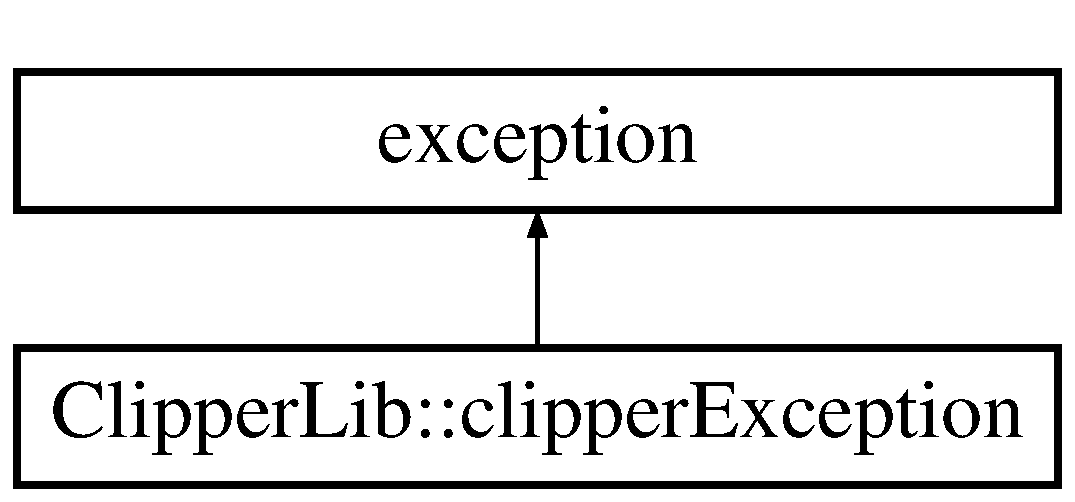
\includegraphics[height=2.000000cm]{class_clipper_lib_1_1clipper_exception}
\end{center}
\end{figure}
\subsection*{Public Member Functions}
\begin{DoxyCompactItemize}
\item 
\hypertarget{class_clipper_lib_1_1clipper_exception_a7d44b32d06cd870500355667f6e0d6ed}{}\label{class_clipper_lib_1_1clipper_exception_a7d44b32d06cd870500355667f6e0d6ed} 
{\bfseries clipper\+Exception} (const char $\ast$description)
\item 
\hypertarget{class_clipper_lib_1_1clipper_exception_a32b7ac5a3176d9040ef0a863fd54657a}{}\label{class_clipper_lib_1_1clipper_exception_a32b7ac5a3176d9040ef0a863fd54657a} 
virtual const char $\ast$ {\bfseries what} () const  throw ()
\end{DoxyCompactItemize}


The documentation for this class was generated from the following file\+:\begin{DoxyCompactItemize}
\item 
C\+:/\+Users/lukas/\+Desktop/\+Road\+Gen\+L\+Systems/Clipper.\+h\end{DoxyCompactItemize}

\hypertarget{class_clipper_lib_1_1_clipper_offset}{}\section{Clipper\+Lib\+:\+:Clipper\+Offset Class Reference}
\label{class_clipper_lib_1_1_clipper_offset}\index{Clipper\+Lib\+::\+Clipper\+Offset@{Clipper\+Lib\+::\+Clipper\+Offset}}
\subsection*{Public Member Functions}
\begin{DoxyCompactItemize}
\item 
\hypertarget{class_clipper_lib_1_1_clipper_offset_a45b4750989901db0c3865c374abdfcdc}{}\label{class_clipper_lib_1_1_clipper_offset_a45b4750989901db0c3865c374abdfcdc} 
{\bfseries Clipper\+Offset} (double miter\+Limit=2.\+0, double round\+Precision=0.\+25)
\item 
\hypertarget{class_clipper_lib_1_1_clipper_offset_a0cd68e3690072f510924a5b25291043b}{}\label{class_clipper_lib_1_1_clipper_offset_a0cd68e3690072f510924a5b25291043b} 
void {\bfseries Add\+Path} (const Path \&path, Join\+Type join\+Type, End\+Type end\+Type)
\item 
\hypertarget{class_clipper_lib_1_1_clipper_offset_a18b35198f6370d76885af995ee2f16cb}{}\label{class_clipper_lib_1_1_clipper_offset_a18b35198f6370d76885af995ee2f16cb} 
void {\bfseries Add\+Paths} (const Paths \&paths, Join\+Type join\+Type, End\+Type end\+Type)
\item 
\hypertarget{class_clipper_lib_1_1_clipper_offset_ac591b25e483a52c99c3190a256ad4589}{}\label{class_clipper_lib_1_1_clipper_offset_ac591b25e483a52c99c3190a256ad4589} 
void {\bfseries Execute} (Paths \&solution, double delta)
\item 
\hypertarget{class_clipper_lib_1_1_clipper_offset_a3aaa9fcc20e503c967a23f1793536118}{}\label{class_clipper_lib_1_1_clipper_offset_a3aaa9fcc20e503c967a23f1793536118} 
void {\bfseries Execute} (\hyperlink{class_clipper_lib_1_1_poly_tree}{Poly\+Tree} \&solution, double delta)
\item 
\hypertarget{class_clipper_lib_1_1_clipper_offset_ab444433587b6a3f6c89655938d889c7d}{}\label{class_clipper_lib_1_1_clipper_offset_ab444433587b6a3f6c89655938d889c7d} 
void {\bfseries Clear} ()
\end{DoxyCompactItemize}
\subsection*{Public Attributes}
\begin{DoxyCompactItemize}
\item 
\hypertarget{class_clipper_lib_1_1_clipper_offset_a36b3bf4571e5b831edd584cbcb179246}{}\label{class_clipper_lib_1_1_clipper_offset_a36b3bf4571e5b831edd584cbcb179246} 
double {\bfseries Miter\+Limit}
\item 
\hypertarget{class_clipper_lib_1_1_clipper_offset_a6c1735720b06e6b92dc25891014b2a92}{}\label{class_clipper_lib_1_1_clipper_offset_a6c1735720b06e6b92dc25891014b2a92} 
double {\bfseries Arc\+Tolerance}
\end{DoxyCompactItemize}


The documentation for this class was generated from the following files\+:\begin{DoxyCompactItemize}
\item 
C\+:/\+Users/lukas/\+Desktop/\+Road\+Gen\+L\+Systems/Clipper.\+h\item 
C\+:/\+Users/lukas/\+Desktop/\+Road\+Gen\+L\+Systems/Clipper.\+cpp\end{DoxyCompactItemize}

\hypertarget{struct_clipper_lib_1_1_double_point}{}\section{Clipper\+Lib\+:\+:Double\+Point Struct Reference}
\label{struct_clipper_lib_1_1_double_point}\index{Clipper\+Lib\+::\+Double\+Point@{Clipper\+Lib\+::\+Double\+Point}}
\subsection*{Public Member Functions}
\begin{DoxyCompactItemize}
\item 
\hypertarget{struct_clipper_lib_1_1_double_point_a3ccbea6aaf488e0a2d8ac499d2676093}{}\label{struct_clipper_lib_1_1_double_point_a3ccbea6aaf488e0a2d8ac499d2676093} 
{\bfseries Double\+Point} (double x=0, double y=0)
\item 
\hypertarget{struct_clipper_lib_1_1_double_point_afd33c9193b3cf11536936dc933b965a4}{}\label{struct_clipper_lib_1_1_double_point_afd33c9193b3cf11536936dc933b965a4} 
{\bfseries Double\+Point} (\hyperlink{struct_clipper_lib_1_1_int_point}{Int\+Point} ip)
\end{DoxyCompactItemize}
\subsection*{Public Attributes}
\begin{DoxyCompactItemize}
\item 
\hypertarget{struct_clipper_lib_1_1_double_point_a675837cc05f20447313789b82d84ad31}{}\label{struct_clipper_lib_1_1_double_point_a675837cc05f20447313789b82d84ad31} 
double {\bfseries X}
\item 
\hypertarget{struct_clipper_lib_1_1_double_point_a49774a93540882d88448badf37034454}{}\label{struct_clipper_lib_1_1_double_point_a49774a93540882d88448badf37034454} 
double {\bfseries Y}
\end{DoxyCompactItemize}


The documentation for this struct was generated from the following file\+:\begin{DoxyCompactItemize}
\item 
C\+:/\+Users/lukas/\+Desktop/\+Road\+Gen\+L\+Systems/Clipper.\+h\end{DoxyCompactItemize}

\hypertarget{class_entity_container}{}\section{Entity\+Container Class Reference}
\label{class_entity_container}\index{Entity\+Container@{Entity\+Container}}


Singleton Container class used by all \hyperlink{class_non_terminal_symbol}{Non\+Terminal\+Symbol} classes.  




{\ttfamily \#include $<$Entity\+Container.\+h$>$}

\subsection*{Public Member Functions}
\begin{DoxyCompactItemize}
\item 
Point\+\_\+2 \hyperlink{class_entity_container_a9a7c554edd1f83a1be2616c0136e42c5}{get\+Grid\+Cell} (C\+G\+A\+L\+::\+M\+P\+\_\+\+Float x, C\+G\+A\+L\+::\+M\+P\+\_\+\+Float y)
\begin{DoxyCompactList}\small\item\em Gets grid cell depending on x and y coordinate. \end{DoxyCompactList}\item 
\hypertarget{class_entity_container_aef2b963be52ce8e8dde81cba5e794834}{}\label{class_entity_container_aef2b963be52ce8e8dde81cba5e794834} 
void \hyperlink{class_entity_container_aef2b963be52ce8e8dde81cba5e794834}{insert\+Street\+Segment} (Segment\+\_\+2 new\+\_\+segment)
\begin{DoxyCompactList}\small\item\em Insert new street segment into grid-\/system. \end{DoxyCompactList}\item 
\hypertarget{class_entity_container_a06738ee0c18eca47bf79a90ee56b8be6}{}\label{class_entity_container_a06738ee0c18eca47bf79a90ee56b8be6} 
void \hyperlink{class_entity_container_a06738ee0c18eca47bf79a90ee56b8be6}{insert\+Intersection} (Point\+\_\+2 intersection)
\begin{DoxyCompactList}\small\item\em Insert new intersection into grid-\/system. \end{DoxyCompactList}\item 
\hypertarget{class_entity_container_a34870620ebef8b20c7685e03e5fde022}{}\label{class_entity_container_a34870620ebef8b20c7685e03e5fde022} 
void \hyperlink{class_entity_container_a34870620ebef8b20c7685e03e5fde022}{insert\+River\+Segment} (Segment\+\_\+2 new\+\_\+segment)
\begin{DoxyCompactList}\small\item\em Insert new river segment into grid-\/system. \end{DoxyCompactList}\item 
Point\+\_\+2 \hyperlink{class_entity_container_a1e1faca63c2c26689c6d49b42edb1792}{segment\+Intersected} (C\+G\+A\+L\+::\+M\+P\+\_\+\+Float x, C\+G\+A\+L\+::\+M\+P\+\_\+\+Float y, C\+G\+A\+L\+::\+M\+P\+\_\+\+Float x\+\_\+new, C\+G\+A\+L\+::\+M\+P\+\_\+\+Float y\+\_\+new, unsigned old\+\_\+angle, int x\+\_\+off, int y\+\_\+off)
\begin{DoxyCompactList}\small\item\em Checks if segment intersects with another one. \end{DoxyCompactList}\item 
Point\+\_\+2 \hyperlink{class_entity_container_a784de18b1f33fa8badc79fc369d29935}{get\+Nearest\+Intersection} (C\+G\+A\+L\+::\+M\+P\+\_\+\+Float x, C\+G\+A\+L\+::\+M\+P\+\_\+\+Float y)
\begin{DoxyCompactList}\small\item\em Gets the nearest intersection. \end{DoxyCompactList}\item 
std\+::vector$<$ Point\+\_\+2 $>$ \hyperlink{class_entity_container_a652c1d48db6052d1d8dd5e1aa5c5eb5f}{river\+Intersected} (C\+G\+A\+L\+::\+M\+P\+\_\+\+Float x, C\+G\+A\+L\+::\+M\+P\+\_\+\+Float y, C\+G\+A\+L\+::\+M\+P\+\_\+\+Float x\+\_\+new, C\+G\+A\+L\+::\+M\+P\+\_\+\+Float y\+\_\+new, int x\+\_\+off, int y\+\_\+off)
\begin{DoxyCompactList}\small\item\em Checks if an existin river would be intersected by inserting the point specified by the paramters. \end{DoxyCompactList}\end{DoxyCompactItemize}
\subsection*{Static Public Member Functions}
\begin{DoxyCompactItemize}
\item 
\hypertarget{class_entity_container_a5b91deaecedcddb382a133904cd1629b}{}\label{class_entity_container_a5b91deaecedcddb382a133904cd1629b} 
static \hyperlink{class_entity_container}{Entity\+Container} $\ast$ {\bfseries get\+Instance} ()
\end{DoxyCompactItemize}
\subsection*{Public Attributes}
\begin{DoxyCompactItemize}
\item 
\hypertarget{class_entity_container_ad5ebeef93ac2c3df991383039e73d5e5}{}\label{class_entity_container_ad5ebeef93ac2c3df991383039e73d5e5} 
unsigned \hyperlink{class_entity_container_ad5ebeef93ac2c3df991383039e73d5e5}{B\+R\+A\+N\+C\+H\+\_\+\+P\+R\+OB} = 88
\begin{DoxyCompactList}\small\item\em Pobability that subsegment branches. \end{DoxyCompactList}\item 
\hypertarget{class_entity_container_ab201ce470dae448f360531fb0e365ce9}{}\label{class_entity_container_ab201ce470dae448f360531fb0e365ce9} 
unsigned \hyperlink{class_entity_container_ab201ce470dae448f360531fb0e365ce9}{L\+I\+G\+H\+T\+\_\+\+P\+R\+OB} = 33
\begin{DoxyCompactList}\small\item\em Probability that lights will be created. \end{DoxyCompactList}\item 
\hypertarget{class_entity_container_af000c1305f9b529e4602022283c4d9f4}{}\label{class_entity_container_af000c1305f9b529e4602022283c4d9f4} 
unsigned \hyperlink{class_entity_container_af000c1305f9b529e4602022283c4d9f4}{N\+U\+M\+B\+\_\+\+R\+I\+V\+E\+RS} = 0
\begin{DoxyCompactList}\small\item\em Number of rivers. \end{DoxyCompactList}\item 
\hypertarget{class_entity_container_a7e9db16fece8ec49c6ec9b8eecb50c12}{}\label{class_entity_container_a7e9db16fece8ec49c6ec9b8eecb50c12} 
unsigned \hyperlink{class_entity_container_a7e9db16fece8ec49c6ec9b8eecb50c12}{M\+A\+X\+\_\+X} = 600
\begin{DoxyCompactList}\small\item\em X-\/\+Dimension of output grid. \end{DoxyCompactList}\item 
\hypertarget{class_entity_container_a78898c6f284910209e9f7a869262fb98}{}\label{class_entity_container_a78898c6f284910209e9f7a869262fb98} 
unsigned \hyperlink{class_entity_container_a78898c6f284910209e9f7a869262fb98}{M\+A\+X\+\_\+Y} = 800
\begin{DoxyCompactList}\small\item\em Y-\/\+Dimension of output grid. \end{DoxyCompactList}\item 
\hypertarget{class_entity_container_aa30630d7b19fdf3eca17f07ef0d8ee28}{}\label{class_entity_container_aa30630d7b19fdf3eca17f07ef0d8ee28} 
int \hyperlink{class_entity_container_aa30630d7b19fdf3eca17f07ef0d8ee28}{M\+A\+X\+\_\+\+S\+E\+G\+\_\+\+C\+O\+U\+NT} = 8000
\begin{DoxyCompactList}\small\item\em Creation threshold. \end{DoxyCompactList}\item 
\hypertarget{class_entity_container_ac3fadec692c82ab047c12137e5c3938d}{}\label{class_entity_container_ac3fadec692c82ab047c12137e5c3938d} 
int {\bfseries M\+A\+X\+\_\+\+S\+E\+G\+\_\+\+C\+O\+U\+N\+T\+\_\+\+I\+N\+IT} = 8000
\item 
int \hyperlink{class_entity_container_a903b71e2c4be9c3e1d09f15e43535117}{D\+A\+Y\+\_\+\+M\+O\+DE} = true
\item 
int \hyperlink{class_entity_container_a9e2ee21384cc1ed4a2a74a2dbb57afa2}{H\+I\+G\+H\+W\+A\+Y\+\_\+\+C\+O\+U\+NT}
\item 
\hypertarget{class_entity_container_aef7e8c301071323d9931070e51404705}{}\label{class_entity_container_aef7e8c301071323d9931070e51404705} 
std\+::vector$<$ Point\+\_\+2 $>$ \hyperlink{class_entity_container_aef7e8c301071323d9931070e51404705}{high\+\_\+dens\+\_\+points\+\_\+}
\begin{DoxyCompactList}\small\item\em Highway goal points. \end{DoxyCompactList}\item 
\hypertarget{class_entity_container_a40984f7d116b526a0bb6eeb987df4014}{}\label{class_entity_container_a40984f7d116b526a0bb6eeb987df4014} 
std\+::vector$<$ Point\+\_\+2 $>$ \hyperlink{class_entity_container_a40984f7d116b526a0bb6eeb987df4014}{start\+\_\+points\+\_\+}
\begin{DoxyCompactList}\small\item\em Highway start points. \end{DoxyCompactList}\item 
\hypertarget{class_entity_container_afdce0409c51b6e1886bb96617ce8d004}{}\label{class_entity_container_afdce0409c51b6e1886bb96617ce8d004} 
std\+::vector$<$ Point\+\_\+2 $>$ \hyperlink{class_entity_container_afdce0409c51b6e1886bb96617ce8d004}{all\+\_\+intersection\+\_\+}
\begin{DoxyCompactList}\small\item\em Container for all intersections (Street and Highway) \end{DoxyCompactList}\item 
\hypertarget{class_entity_container_af4e20ae8193a2b910f8a928dc72cbd75}{}\label{class_entity_container_af4e20ae8193a2b910f8a928dc72cbd75} 
std\+::vector$<$ Segment\+\_\+2 $>$ \hyperlink{class_entity_container_af4e20ae8193a2b910f8a928dc72cbd75}{all\+\_\+street\+\_\+segments\+\_\+}
\begin{DoxyCompactList}\small\item\em Container for all street segments. \end{DoxyCompactList}\item 
\hypertarget{class_entity_container_ae2d78a8360b2ebf66c537f4659fc4d75}{}\label{class_entity_container_ae2d78a8360b2ebf66c537f4659fc4d75} 
std\+::vector$<$ Point\+\_\+2 $>$ \hyperlink{class_entity_container_ae2d78a8360b2ebf66c537f4659fc4d75}{all\+\_\+highway\+\_\+intersections\+\_\+}
\begin{DoxyCompactList}\small\item\em Container for all highway intersections. \end{DoxyCompactList}\item 
\hypertarget{class_entity_container_a674902cc4f07335f3a241e10aa3d6456}{}\label{class_entity_container_a674902cc4f07335f3a241e10aa3d6456} 
std\+::vector$<$ Point\+\_\+2 $>$ \hyperlink{class_entity_container_a674902cc4f07335f3a241e10aa3d6456}{all\+\_\+highway\+\_\+exits\+\_\+}
\begin{DoxyCompactList}\small\item\em Container for all highway exits (branch points) \end{DoxyCompactList}\item 
\hypertarget{class_entity_container_ac63e745f9bff741c72f413141a8f9b94}{}\label{class_entity_container_ac63e745f9bff741c72f413141a8f9b94} 
std\+::vector$<$ Segment\+\_\+2 $>$ \hyperlink{class_entity_container_ac63e745f9bff741c72f413141a8f9b94}{all\+\_\+highway\+\_\+segments\+\_\+}
\begin{DoxyCompactList}\small\item\em Container for all highway segments. \end{DoxyCompactList}\item 
\hypertarget{class_entity_container_a73a5483cb36051add961774e28fb086c}{}\label{class_entity_container_a73a5483cb36051add961774e28fb086c} 
std\+::vector$<$ Segment\+\_\+2 $>$ \hyperlink{class_entity_container_a73a5483cb36051add961774e28fb086c}{river\+\_\+segments\+\_\+}
\begin{DoxyCompactList}\small\item\em Container for all river segments. \end{DoxyCompactList}\item 
\hypertarget{class_entity_container_aea99d9281974632801f8e8274d5e35ac}{}\label{class_entity_container_aea99d9281974632801f8e8274d5e35ac} 
std\+::vector$<$ Segment\+\_\+2 $>$ \hyperlink{class_entity_container_aea99d9281974632801f8e8274d5e35ac}{bridges\+\_\+}
\begin{DoxyCompactList}\small\item\em Container for all bridges. \end{DoxyCompactList}\item 
std\+::vector$<$ std\+::vector$<$ Point\+\_\+2 $>$ $>$ \hyperlink{class_entity_container_a5f33573ae189549588fe11c9207374f7}{all\+\_\+polygons\+\_\+}
\item 
\hypertarget{class_entity_container_a6817baf3af18e5fcb1ed10524c5f4998}{}\label{class_entity_container_a6817baf3af18e5fcb1ed10524c5f4998} 
std\+::vector$<$ std\+::vector$<$ Point\+\_\+2 $>$ $>$ {\bfseries all\+\_\+green\+\_\+spaces\+\_\+}
\item 
\hypertarget{class_entity_container_a38ac59ad4909159a66142c86fcb47f23}{}\label{class_entity_container_a38ac59ad4909159a66142c86fcb47f23} 
std\+::vector$<$ std\+::vector$<$ Point\+\_\+2 $>$ $>$ {\bfseries all\+\_\+lots\+\_\+}
\item 
\hypertarget{class_entity_container_abb6d78fdd55d0b20136281831bc27d47}{}\label{class_entity_container_abb6d78fdd55d0b20136281831bc27d47} 
std\+::vector$<$ std\+::vector$<$ Point\+\_\+2 $>$ $>$ {\bfseries all\+\_\+parking\+\_\+lots\+\_\+}
\item 
\hypertarget{class_entity_container_a995fab173a1188bf9798c762e265a94b}{}\label{class_entity_container_a995fab173a1188bf9798c762e265a94b} 
std\+::vector$<$ std\+::vector$<$ Point\+\_\+2 $>$ $>$ {\bfseries all\+\_\+rivers\+\_\+}
\item 
\hypertarget{class_entity_container_a17f869e37db8fe181f2634829c4542b1}{}\label{class_entity_container_a17f869e37db8fe181f2634829c4542b1} 
std\+::vector$<$ std\+::vector$<$ Point\+\_\+2 $>$ $>$ {\bfseries all\+\_\+trees\+\_\+}
\item 
\hypertarget{class_entity_container_ae5c82ecd330a6dfac1cc2b472fa25723}{}\label{class_entity_container_ae5c82ecd330a6dfac1cc2b472fa25723} 
std\+::vector$<$ std\+::vector$<$ Point\+\_\+2 $>$ $>$ {\bfseries all\+\_\+lights\+\_\+}
\item 
\hypertarget{class_entity_container_abd407f32b3116ef9e295a30eaf3b1fb4}{}\label{class_entity_container_abd407f32b3116ef9e295a30eaf3b1fb4} 
std\+::map$<$ Point\+\_\+2, std\+::vector$<$ Point\+\_\+2 $>$ $>$ {\bfseries all\+\_\+parks\+\_\+}
\item 
\hypertarget{class_entity_container_af5838a14b7b62083462aa908d6051f68}{}\label{class_entity_container_af5838a14b7b62083462aa908d6051f68} 
std\+::map$<$ double, std\+::vector$<$ Point\+\_\+2 $>$ $>$ {\bfseries possible\+\_\+parks\+\_\+}
\item 
std\+::vector$<$ Segment\+\_\+2 $>$ \hyperlink{class_entity_container_ada172611f1ac17c72a201122bec06796}{all\+\_\+highway\+\_\+poly\+\_\+segments\+\_\+}
\begin{DoxyCompactList}\small\item\em Segments for polygon creation. \end{DoxyCompactList}\item 
\hypertarget{class_entity_container_a2d13b673d7e3dfd5d6e32bcb43f55e6c}{}\label{class_entity_container_a2d13b673d7e3dfd5d6e32bcb43f55e6c} 
std\+::vector$<$ Segment\+\_\+2 $>$ {\bfseries all\+\_\+street\+\_\+poly\+\_\+segments\+\_\+}
\item 
std\+::vector$<$ Segment\+\_\+2 $>$ \hyperlink{class_entity_container_a3ef34e622b3fa04986935d20c503ae53}{street\+\_\+segment\+\_\+grid} \mbox{[}100\mbox{]}\mbox{[}100\mbox{]}
\begin{DoxyCompactList}\small\item\em Grid used for neighbour detection. \end{DoxyCompactList}\item 
\hypertarget{class_entity_container_a82488b4b59d1cfb8a94ca2579ada935c}{}\label{class_entity_container_a82488b4b59d1cfb8a94ca2579ada935c} 
std\+::vector$<$ Point\+\_\+2 $>$ \hyperlink{class_entity_container_a82488b4b59d1cfb8a94ca2579ada935c}{intersection\+\_\+grid} \mbox{[}100\mbox{]}\mbox{[}100\mbox{]}
\begin{DoxyCompactList}\small\item\em Grid used for intersection point. See street\+\_\+segment\+\_\+grid for further explanantion. \end{DoxyCompactList}\item 
\hypertarget{class_entity_container_a66ebc4d45f6b543b4d1fca1fdd69de58}{}\label{class_entity_container_a66ebc4d45f6b543b4d1fca1fdd69de58} 
std\+::vector$<$ Segment\+\_\+2 $>$ \hyperlink{class_entity_container_a66ebc4d45f6b543b4d1fca1fdd69de58}{river\+\_\+segment\+\_\+grid} \mbox{[}100\mbox{]}\mbox{[}100\mbox{]}
\begin{DoxyCompactList}\small\item\em Grid used for river segments. See street\+\_\+segment\+\_\+grid for further explanantion. \end{DoxyCompactList}\end{DoxyCompactItemize}


\subsection{Detailed Description}
Singleton Container class used by all \hyperlink{class_non_terminal_symbol}{Non\+Terminal\+Symbol} classes. 

Holds all segments, all intersection and other needed informations. Class is a singleton and is used allover the project as a {\bfseries shared} {\bfseries information} {\bfseries container} (if necessary).

\begin{DoxyNote}{Note}
Also holds functions for intersection checking 

Some variables will be read from input file (capitalized variables)
\end{DoxyNote}
\begin{DoxyAuthor}{Author}
Lukas Gregori 
\end{DoxyAuthor}
\begin{DoxyVersion}{Version}

\end{DoxyVersion}
\begin{DoxyParagraph}{Revision}
1.\+0 
\end{DoxyParagraph}


Contact\+: \href{mailto:lukas.gregori@student.tugraz.at}{\tt lukas.\+gregori@student.\+tugraz.\+at}

Class implemented as singleton 

 Copyright (C) Lukas Gregori, \href{mailto:contact@lukasgregori.com}{\tt contact@lukasgregori.\+com}

This file is part of the road network generator Road\+Gen.

Road\+Gen is free software\+: you can redistribute it and/or modify it under the terms of the G\+NU General Public License as published by the Free Software Foundation, either version 3 of the License, or (at your option) any later version.

Road\+Gen is distributed in the hope that it will be useful, but W\+I\+T\+H\+O\+UT A\+NY W\+A\+R\+R\+A\+N\+TY; without even the implied warranty of M\+E\+R\+C\+H\+A\+N\+T\+A\+B\+I\+L\+I\+TY or F\+I\+T\+N\+E\+SS F\+OR A P\+A\+R\+T\+I\+C\+U\+L\+AR P\+U\+R\+P\+O\+SE. See the G\+NU General Public License for more details.

You should have received a copy of the G\+NU General Public License \subsubsection*{along with Foobar. If not, see \href{http://www.gnu.org/licenses/}{\tt http\+://www.\+gnu.\+org/licenses/}. }

\subsection{Member Function Documentation}
\hypertarget{class_entity_container_a9a7c554edd1f83a1be2616c0136e42c5}{}\label{class_entity_container_a9a7c554edd1f83a1be2616c0136e42c5} 
\index{Entity\+Container@{Entity\+Container}!get\+Grid\+Cell@{get\+Grid\+Cell}}
\index{get\+Grid\+Cell@{get\+Grid\+Cell}!Entity\+Container@{Entity\+Container}}
\subsubsection{\texorpdfstring{get\+Grid\+Cell()}{getGridCell()}}
{\footnotesize\ttfamily Point\+\_\+2 Entity\+Container\+::get\+Grid\+Cell (\begin{DoxyParamCaption}\item[{C\+G\+A\+L\+::\+M\+P\+\_\+\+Float}]{x,  }\item[{C\+G\+A\+L\+::\+M\+P\+\_\+\+Float}]{y }\end{DoxyParamCaption})}



Gets grid cell depending on x and y coordinate. 

Returns the indizes of the grid cell in which x and y belong. Cann be used as index to the points grid.


\begin{DoxyParams}{Parameters}
{\em C\+G\+A\+L\+::\+M\+P\+\_\+\+Float} & x x-\/coordinate \\
\hline
{\em C\+G\+A\+L\+::\+M\+P\+\_\+\+Float} & y y-\/coordinate\\
\hline
\end{DoxyParams}
\begin{DoxyReturn}{Returns}
Point\+\_\+2 The cell the coordinates are in 
\end{DoxyReturn}
\hypertarget{class_entity_container_a784de18b1f33fa8badc79fc369d29935}{}\label{class_entity_container_a784de18b1f33fa8badc79fc369d29935} 
\index{Entity\+Container@{Entity\+Container}!get\+Nearest\+Intersection@{get\+Nearest\+Intersection}}
\index{get\+Nearest\+Intersection@{get\+Nearest\+Intersection}!Entity\+Container@{Entity\+Container}}
\subsubsection{\texorpdfstring{get\+Nearest\+Intersection()}{getNearestIntersection()}}
{\footnotesize\ttfamily Point\+\_\+2 Entity\+Container\+::get\+Nearest\+Intersection (\begin{DoxyParamCaption}\item[{C\+G\+A\+L\+::\+M\+P\+\_\+\+Float}]{x,  }\item[{C\+G\+A\+L\+::\+M\+P\+\_\+\+Float}]{y }\end{DoxyParamCaption})}



Gets the nearest intersection. 

Calculates the nearest intersection point (if found), by using the grid system from the \hyperlink{class_entity_container}{Entity\+Container} class.

If no intersection could be detected, the method returns P(0,0)


\begin{DoxyParams}{Parameters}
{\em C\+G\+A\+L\+::\+M\+P\+\_\+\+Float} & x Coordinate of P\+OI \\
\hline
{\em C\+G\+A\+L\+::\+M\+P\+\_\+\+Float} & y Coordinate of P\+OI \\
\hline
{\em int} & x\+\_\+off Grid Range X \\
\hline
{\em int} & y\+\_\+off Grid Range Y\\
\hline
\end{DoxyParams}
\begin{DoxyReturn}{Returns}
Point\+\_\+2 the next closest interception\+\_\+point, P(0,0) if no intersection was found 
\end{DoxyReturn}
\hypertarget{class_entity_container_a652c1d48db6052d1d8dd5e1aa5c5eb5f}{}\label{class_entity_container_a652c1d48db6052d1d8dd5e1aa5c5eb5f} 
\index{Entity\+Container@{Entity\+Container}!river\+Intersected@{river\+Intersected}}
\index{river\+Intersected@{river\+Intersected}!Entity\+Container@{Entity\+Container}}
\subsubsection{\texorpdfstring{river\+Intersected()}{riverIntersected()}}
{\footnotesize\ttfamily std\+::vector$<$ Point\+\_\+2 $>$ Entity\+Container\+::river\+Intersected (\begin{DoxyParamCaption}\item[{C\+G\+A\+L\+::\+M\+P\+\_\+\+Float}]{x,  }\item[{C\+G\+A\+L\+::\+M\+P\+\_\+\+Float}]{y,  }\item[{C\+G\+A\+L\+::\+M\+P\+\_\+\+Float}]{x\+\_\+new,  }\item[{C\+G\+A\+L\+::\+M\+P\+\_\+\+Float}]{y\+\_\+new,  }\item[{int}]{x\+\_\+off,  }\item[{int}]{y\+\_\+off }\end{DoxyParamCaption})}



Checks if an existin river would be intersected by inserting the point specified by the paramters. 


\begin{DoxyParams}{Parameters}
{\em C\+G\+A\+L\+::\+M\+P\+\_\+\+Float} & x start X of new segment \\
\hline
{\em C\+G\+A\+L\+::\+M\+P\+\_\+\+Float} & y start Y of new segment \\
\hline
{\em C\+G\+A\+L\+::\+M\+P\+\_\+\+Float} & x\+\_\+new end X of new segment \\
\hline
{\em C\+G\+A\+L\+::\+M\+P\+\_\+\+Float} & y\+\_\+new end Y of new segment \\
\hline
{\em int} & x\+\_\+off, int y\+\_\+off Grid offset\\
\hline
\end{DoxyParams}
Point\+\_\+2 the next closest interception\+\_\+point, P(0,0) if no intersection was found \hypertarget{class_entity_container_a1e1faca63c2c26689c6d49b42edb1792}{}\label{class_entity_container_a1e1faca63c2c26689c6d49b42edb1792} 
\index{Entity\+Container@{Entity\+Container}!segment\+Intersected@{segment\+Intersected}}
\index{segment\+Intersected@{segment\+Intersected}!Entity\+Container@{Entity\+Container}}
\subsubsection{\texorpdfstring{segment\+Intersected()}{segmentIntersected()}}
{\footnotesize\ttfamily Point\+\_\+2 Entity\+Container\+::segment\+Intersected (\begin{DoxyParamCaption}\item[{C\+G\+A\+L\+::\+M\+P\+\_\+\+Float}]{x,  }\item[{C\+G\+A\+L\+::\+M\+P\+\_\+\+Float}]{y,  }\item[{C\+G\+A\+L\+::\+M\+P\+\_\+\+Float}]{x\+\_\+new,  }\item[{C\+G\+A\+L\+::\+M\+P\+\_\+\+Float}]{y\+\_\+new,  }\item[{unsigned}]{old\+\_\+angle,  }\item[{int}]{x\+\_\+off,  }\item[{int}]{y\+\_\+off }\end{DoxyParamCaption})}



Checks if segment intersects with another one. 

Checks if the segment which starts at x/y and ends at x\+\_\+new/y\+\_\+new intersects with any other segment within a hard-\/coded range.

If the segment intercepts with one other segments, the closest interception point is returned


\begin{DoxyParams}{Parameters}
{\em C\+G\+A\+L\+::\+M\+P\+\_\+\+Float} & x start X of new segment \\
\hline
{\em C\+G\+A\+L\+::\+M\+P\+\_\+\+Float} & y start Y of new segment \\
\hline
{\em C\+G\+A\+L\+::\+M\+P\+\_\+\+Float} & x\+\_\+new end X of new segment \\
\hline
{\em C\+G\+A\+L\+::\+M\+P\+\_\+\+Float} & y\+\_\+new end Y of new segment \\
\hline
{\em unsigned} & old\+\_\+angle angle (Intersection merging) \\
\hline
{\em int} & x\+\_\+off Grid Range X \\
\hline
{\em int} & y\+\_\+off Grid Range Y\\
\hline
\end{DoxyParams}
\begin{DoxyReturn}{Returns}
Point\+\_\+2 the next closest interception\+\_\+point, P(0,0) if no intersection was found 
\end{DoxyReturn}


\subsection{Member Data Documentation}
\hypertarget{class_entity_container_ada172611f1ac17c72a201122bec06796}{}\label{class_entity_container_ada172611f1ac17c72a201122bec06796} 
\index{Entity\+Container@{Entity\+Container}!all\+\_\+highway\+\_\+poly\+\_\+segments\+\_\+@{all\+\_\+highway\+\_\+poly\+\_\+segments\+\_\+}}
\index{all\+\_\+highway\+\_\+poly\+\_\+segments\+\_\+@{all\+\_\+highway\+\_\+poly\+\_\+segments\+\_\+}!Entity\+Container@{Entity\+Container}}
\subsubsection{\texorpdfstring{all\+\_\+highway\+\_\+poly\+\_\+segments\+\_\+}{all\_highway\_poly\_segments\_}}
{\footnotesize\ttfamily std\+::vector$<$Segment\+\_\+2$>$ Entity\+Container\+::all\+\_\+highway\+\_\+poly\+\_\+segments\+\_\+}



Segments for polygon creation. 

Stores the segments needed for the polygon creation. We create a seperate vector which does not stop at intersections, but rather continues drawing a bit, so that the 2\+D-\/\+Arrangements can detect an intersection \hypertarget{class_entity_container_a5f33573ae189549588fe11c9207374f7}{}\label{class_entity_container_a5f33573ae189549588fe11c9207374f7} 
\index{Entity\+Container@{Entity\+Container}!all\+\_\+polygons\+\_\+@{all\+\_\+polygons\+\_\+}}
\index{all\+\_\+polygons\+\_\+@{all\+\_\+polygons\+\_\+}!Entity\+Container@{Entity\+Container}}
\subsubsection{\texorpdfstring{all\+\_\+polygons\+\_\+}{all\_polygons\_}}
{\footnotesize\ttfamily std\+::vector$<$std\+::vector$<$Point\+\_\+2$>$ $>$ Entity\+Container\+::all\+\_\+polygons\+\_\+}

All polygons gotten from the J\+S\+O\+N-\/\+Generator using the line segments from the ...\+\_\+poly\+\_\+segments vectors below. \hypertarget{class_entity_container_a903b71e2c4be9c3e1d09f15e43535117}{}\label{class_entity_container_a903b71e2c4be9c3e1d09f15e43535117} 
\index{Entity\+Container@{Entity\+Container}!D\+A\+Y\+\_\+\+M\+O\+DE@{D\+A\+Y\+\_\+\+M\+O\+DE}}
\index{D\+A\+Y\+\_\+\+M\+O\+DE@{D\+A\+Y\+\_\+\+M\+O\+DE}!Entity\+Container@{Entity\+Container}}
\subsubsection{\texorpdfstring{D\+A\+Y\+\_\+\+M\+O\+DE}{DAY\_MODE}}
{\footnotesize\ttfamily int Entity\+Container\+::\+D\+A\+Y\+\_\+\+M\+O\+DE = true}

Dependant on this variable an export flag is set for the city generator (G\+ML), which will then handle the textures for the windows differently (Will emitt light). \hypertarget{class_entity_container_a9e2ee21384cc1ed4a2a74a2dbb57afa2}{}\label{class_entity_container_a9e2ee21384cc1ed4a2a74a2dbb57afa2} 
\index{Entity\+Container@{Entity\+Container}!H\+I\+G\+H\+W\+A\+Y\+\_\+\+C\+O\+U\+NT@{H\+I\+G\+H\+W\+A\+Y\+\_\+\+C\+O\+U\+NT}}
\index{H\+I\+G\+H\+W\+A\+Y\+\_\+\+C\+O\+U\+NT@{H\+I\+G\+H\+W\+A\+Y\+\_\+\+C\+O\+U\+NT}!Entity\+Container@{Entity\+Container}}
\subsubsection{\texorpdfstring{H\+I\+G\+H\+W\+A\+Y\+\_\+\+C\+O\+U\+NT}{HIGHWAY\_COUNT}}
{\footnotesize\ttfamily int Entity\+Container\+::\+H\+I\+G\+H\+W\+A\+Y\+\_\+\+C\+O\+U\+NT}

Number of highways total. Used for street-\/start creation. Streets may only propagate (\char`\"{}grow\char`\"{}) once all highways were closed. \hypertarget{class_entity_container_a3ef34e622b3fa04986935d20c503ae53}{}\label{class_entity_container_a3ef34e622b3fa04986935d20c503ae53} 
\index{Entity\+Container@{Entity\+Container}!street\+\_\+segment\+\_\+grid@{street\+\_\+segment\+\_\+grid}}
\index{street\+\_\+segment\+\_\+grid@{street\+\_\+segment\+\_\+grid}!Entity\+Container@{Entity\+Container}}
\subsubsection{\texorpdfstring{street\+\_\+segment\+\_\+grid}{street\_segment\_grid}}
{\footnotesize\ttfamily std\+::vector$<$Segment\+\_\+2$>$ Entity\+Container\+::street\+\_\+segment\+\_\+grid\mbox{[}100\mbox{]}\mbox{[}100\mbox{]}}



Grid used for neighbour detection. 

If we need the neighbours of one point, we check the corresponding square. We can thus compute the neighbours by a simple lookup operation {\ttfamily }(O(1)) 

The documentation for this class was generated from the following files\+:\begin{DoxyCompactItemize}
\item 
C\+:/\+Users/lukas/\+Desktop/\+Road\+Gen\+L\+Systems/Entity\+Container.\+h\item 
C\+:/\+Users/lukas/\+Desktop/\+Road\+Gen\+L\+Systems/Entity\+Container.\+cpp\end{DoxyCompactItemize}

\hypertarget{class_i_interpretable}{}\section{I\+Interpretable Class Reference}
\label{class_i_interpretable}\index{I\+Interpretable@{I\+Interpretable}}


Interface declares interpretors for the gotten results.  




{\ttfamily \#include $<$I\+Interpretable.\+h$>$}

Inheritance diagram for I\+Interpretable\+:\begin{figure}[H]
\begin{center}
\leavevmode
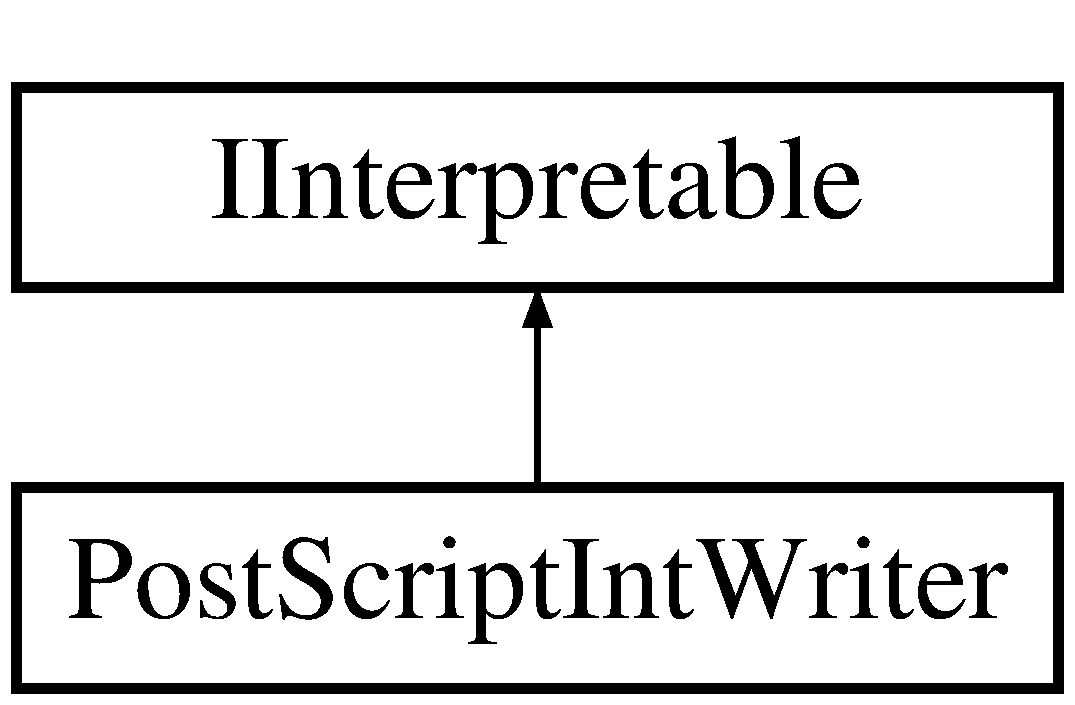
\includegraphics[height=2.000000cm]{class_i_interpretable}
\end{center}
\end{figure}
\subsection*{Public Member Functions}
\begin{DoxyCompactItemize}
\item 
\hypertarget{class_i_interpretable_a111c0b6ed22d2ab516c6ca3fbd709a63}{}\label{class_i_interpretable_a111c0b6ed22d2ab516c6ca3fbd709a63} 
virtual void {\bfseries handle\+River} (std\+::vector$<$ Segment\+\_\+2 $>$ river)=0
\item 
\hypertarget{class_i_interpretable_adfa70e9492340b2095c682dca05b9227}{}\label{class_i_interpretable_adfa70e9492340b2095c682dca05b9227} 
virtual void {\bfseries handle\+Error} (std\+::vector$<$ Segment\+\_\+2 $>$ error)=0
\item 
\hypertarget{class_i_interpretable_a3f7441857e03e16a2ffaaaf214249839}{}\label{class_i_interpretable_a3f7441857e03e16a2ffaaaf214249839} 
virtual void {\bfseries handle\+Bridges} (std\+::vector$<$ Segment\+\_\+2 $>$ bridges)=0
\item 
\hypertarget{class_i_interpretable_aa857e725bb0d2f82a0ee47758bfb1005}{}\label{class_i_interpretable_aa857e725bb0d2f82a0ee47758bfb1005} 
virtual void {\bfseries handle\+Street\+Segments} (std\+::vector$<$ Segment\+\_\+2 $>$ streets)=0
\item 
\hypertarget{class_i_interpretable_a7d266b1337d81a3faca42b987293fb9a}{}\label{class_i_interpretable_a7d266b1337d81a3faca42b987293fb9a} 
virtual void {\bfseries handle\+Highway\+Exit} (C\+G\+A\+L\+::\+M\+P\+\_\+\+Float x, C\+G\+A\+L\+::\+M\+P\+\_\+\+Float y)=0
\item 
\hypertarget{class_i_interpretable_ac1a4695ce8a38f30c72444964528f66f}{}\label{class_i_interpretable_ac1a4695ce8a38f30c72444964528f66f} 
virtual void {\bfseries handle\+Highway\+Segments} (std\+::vector$<$ Segment\+\_\+2 $>$ highways)=0
\item 
\hypertarget{class_i_interpretable_a2e4d9b4686ea4745b228f0455dbfb00c}{}\label{class_i_interpretable_a2e4d9b4686ea4745b228f0455dbfb00c} 
virtual void {\bfseries handle\+New\+Highway\+Start} (C\+G\+A\+L\+::\+M\+P\+\_\+\+Float x, C\+G\+A\+L\+::\+M\+P\+\_\+\+Float y)=0
\item 
\hypertarget{class_i_interpretable_a3f3973a2ab6bd88fe269e9cbb96424e1}{}\label{class_i_interpretable_a3f3973a2ab6bd88fe269e9cbb96424e1} 
virtual void {\bfseries handle\+High\+Density\+Point} (C\+G\+A\+L\+::\+M\+P\+\_\+\+Float x, C\+G\+A\+L\+::\+M\+P\+\_\+\+Float y, int max\+\_\+diameter)=0
\item 
\hypertarget{class_i_interpretable_a19891b709c0b9610ee7e0bc6cfacfa2e}{}\label{class_i_interpretable_a19891b709c0b9610ee7e0bc6cfacfa2e} 
virtual void {\bfseries handle\+Highway\+Interception} (C\+G\+A\+L\+::\+M\+P\+\_\+\+Float x, C\+G\+A\+L\+::\+M\+P\+\_\+\+Float y)=0
\item 
\hypertarget{class_i_interpretable_aa4cdcc0ed84340a98edcdccb1b7b0832}{}\label{class_i_interpretable_aa4cdcc0ed84340a98edcdccb1b7b0832} 
virtual void {\bfseries handle\+Interception} (C\+G\+A\+L\+::\+M\+P\+\_\+\+Float new\+\_\+x, C\+G\+A\+L\+::\+M\+P\+\_\+\+Float new\+\_\+y)=0
\item 
\hypertarget{class_i_interpretable_a8be21dc53a269a2f063dedbef82a5324}{}\label{class_i_interpretable_a8be21dc53a269a2f063dedbef82a5324} 
virtual void {\bfseries handle\+Polygon} (std\+::vector$<$ Point\+\_\+2 $>$ polygon, unsigned r, unsigned g, unsigned b)=0
\item 
\hypertarget{class_i_interpretable_a303b1a1d5b4a8161b3ac949a242d9edd}{}\label{class_i_interpretable_a303b1a1d5b4a8161b3ac949a242d9edd} 
virtual void {\bfseries close\+Network} ()=0
\item 
\hypertarget{class_i_interpretable_a43563bf724954090b618c66a865643fe}{}\label{class_i_interpretable_a43563bf724954090b618c66a865643fe} 
virtual void {\bfseries start\+Network} ()=0
\item 
\hypertarget{class_i_interpretable_aa020c43e83d17a5faa60c7c4d53ebcb5}{}\label{class_i_interpretable_aa020c43e83d17a5faa60c7c4d53ebcb5} 
virtual void {\bfseries close\+File} ()=0
\item 
\hypertarget{class_i_interpretable_a5b7e79c4251dcc50783e1c11b71c6b8c}{}\label{class_i_interpretable_a5b7e79c4251dcc50783e1c11b71c6b8c} 
virtual void {\bfseries open\+File} (std\+::string file\+\_\+name)=0
\item 
\hypertarget{class_i_interpretable_a5a176aa42f975513e3b5bf030c7f34b4}{}\label{class_i_interpretable_a5a176aa42f975513e3b5bf030c7f34b4} 
virtual void \hyperlink{class_i_interpretable_a5a176aa42f975513e3b5bf030c7f34b4}{set\+Background\+Color} (unsigned r, unsigned g, unsigned b)=0
\begin{DoxyCompactList}\small\item\em Set background color of the output map. \end{DoxyCompactList}\end{DoxyCompactItemize}


\subsection{Detailed Description}
Interface declares interpretors for the gotten results. 

\hyperlink{class_i_interpretable}{I\+Interpretable}

Different interpretors could be added (Different output formats). Currently only the \hyperlink{class_post_script_int_writer}{Post\+Script\+Int\+Writer} makes use of this interface

Contains different handler functions for the different data collected throughout the generation, as well as helper functions for creating the network.

\begin{DoxyAuthor}{Author}
Lukas Gregori 
\end{DoxyAuthor}
\begin{DoxyVersion}{Version}

\end{DoxyVersion}
\begin{DoxyParagraph}{Revision}
1.\+0 
\end{DoxyParagraph}


Contact\+: \href{mailto:lukas.gregori@student.tugraz.at}{\tt lukas.\+gregori@student.\+tugraz.\+at}



 Copyright (C) Lukas Gregori, \href{mailto:contact@lukasgregori.com}{\tt contact@lukasgregori.\+com}

This file is part of the road network generator Road\+Gen.

Road\+Gen is free software\+: you can redistribute it and/or modify it under the terms of the G\+NU General Public License as published by the Free Software Foundation, either version 3 of the License, or (at your option) any later version.

Road\+Gen is distributed in the hope that it will be useful, but W\+I\+T\+H\+O\+UT A\+NY W\+A\+R\+R\+A\+N\+TY; without even the implied warranty of M\+E\+R\+C\+H\+A\+N\+T\+A\+B\+I\+L\+I\+TY or F\+I\+T\+N\+E\+SS F\+OR A P\+A\+R\+T\+I\+C\+U\+L\+AR P\+U\+R\+P\+O\+SE. See the G\+NU General Public License for more details.

You should have received a copy of the G\+NU General Public License \subsubsection*{along with Foobar. If not, see \href{http://www.gnu.org/licenses/}{\tt http\+://www.\+gnu.\+org/licenses/}. }

The documentation for this class was generated from the following file\+:\begin{DoxyCompactItemize}
\item 
C\+:/\+Users/lukas/\+Desktop/\+Road\+Gen\+L\+Systems/I\+Interpretable.\+h\end{DoxyCompactItemize}

\hypertarget{class_clipper_lib_1_1_int128}{}\section{Clipper\+Lib\+:\+:Int128 Class Reference}
\label{class_clipper_lib_1_1_int128}\index{Clipper\+Lib\+::\+Int128@{Clipper\+Lib\+::\+Int128}}
\subsection*{Public Member Functions}
\begin{DoxyCompactItemize}
\item 
\hypertarget{class_clipper_lib_1_1_int128_acb7953a56e0ddb6d3245268e457f9e37}{}\label{class_clipper_lib_1_1_int128_acb7953a56e0ddb6d3245268e457f9e37} 
{\bfseries Int128} (long64 \+\_\+lo=0)
\item 
\hypertarget{class_clipper_lib_1_1_int128_ad113c3dc3bd371984b05fddb1fe527e2}{}\label{class_clipper_lib_1_1_int128_ad113c3dc3bd371984b05fddb1fe527e2} 
{\bfseries Int128} (const \hyperlink{class_clipper_lib_1_1_int128}{Int128} \&val)
\item 
\hypertarget{class_clipper_lib_1_1_int128_ac23a17a6a5ea143f0297b7ba0dd1830e}{}\label{class_clipper_lib_1_1_int128_ac23a17a6a5ea143f0297b7ba0dd1830e} 
{\bfseries Int128} (const long64 \&\+\_\+hi, const ulong64 \&\+\_\+lo)
\item 
\hypertarget{class_clipper_lib_1_1_int128_a908b1ffab7e190f8db9d2adccbb9eef4}{}\label{class_clipper_lib_1_1_int128_a908b1ffab7e190f8db9d2adccbb9eef4} 
\hyperlink{class_clipper_lib_1_1_int128}{Int128} \& {\bfseries operator=} (const long64 \&val)
\item 
\hypertarget{class_clipper_lib_1_1_int128_a8946a96471d06371fd5ea4f4f65cb4c9}{}\label{class_clipper_lib_1_1_int128_a8946a96471d06371fd5ea4f4f65cb4c9} 
bool {\bfseries operator==} (const \hyperlink{class_clipper_lib_1_1_int128}{Int128} \&val) const
\item 
\hypertarget{class_clipper_lib_1_1_int128_ae7437e8f6dcb611e8b33e5e7c9c8fbc0}{}\label{class_clipper_lib_1_1_int128_ae7437e8f6dcb611e8b33e5e7c9c8fbc0} 
bool {\bfseries operator!=} (const \hyperlink{class_clipper_lib_1_1_int128}{Int128} \&val) const
\item 
\hypertarget{class_clipper_lib_1_1_int128_ac3d844564066e223483f9393ba050daa}{}\label{class_clipper_lib_1_1_int128_ac3d844564066e223483f9393ba050daa} 
bool {\bfseries operator$>$} (const \hyperlink{class_clipper_lib_1_1_int128}{Int128} \&val) const
\item 
\hypertarget{class_clipper_lib_1_1_int128_ab55bb6a363e7ced8e5e64a1eefac6000}{}\label{class_clipper_lib_1_1_int128_ab55bb6a363e7ced8e5e64a1eefac6000} 
bool {\bfseries operator$<$} (const \hyperlink{class_clipper_lib_1_1_int128}{Int128} \&val) const
\item 
\hypertarget{class_clipper_lib_1_1_int128_af01cfcc3d7bdeffc25e2efb855cd196e}{}\label{class_clipper_lib_1_1_int128_af01cfcc3d7bdeffc25e2efb855cd196e} 
bool {\bfseries operator$>$=} (const \hyperlink{class_clipper_lib_1_1_int128}{Int128} \&val) const
\item 
\hypertarget{class_clipper_lib_1_1_int128_ab3667a2abe7b05841b8004496e4e5ddd}{}\label{class_clipper_lib_1_1_int128_ab3667a2abe7b05841b8004496e4e5ddd} 
bool {\bfseries operator$<$=} (const \hyperlink{class_clipper_lib_1_1_int128}{Int128} \&val) const
\item 
\hypertarget{class_clipper_lib_1_1_int128_ad48a700134ab5c4e08bd53966b731950}{}\label{class_clipper_lib_1_1_int128_ad48a700134ab5c4e08bd53966b731950} 
\hyperlink{class_clipper_lib_1_1_int128}{Int128} \& {\bfseries operator+=} (const \hyperlink{class_clipper_lib_1_1_int128}{Int128} \&rhs)
\item 
\hypertarget{class_clipper_lib_1_1_int128_ad32b1394a82ddf0d9f7da299b91212bd}{}\label{class_clipper_lib_1_1_int128_ad32b1394a82ddf0d9f7da299b91212bd} 
\hyperlink{class_clipper_lib_1_1_int128}{Int128} {\bfseries operator+} (const \hyperlink{class_clipper_lib_1_1_int128}{Int128} \&rhs) const
\item 
\hypertarget{class_clipper_lib_1_1_int128_a7b35c74c15392ae8d48c031f750c1b28}{}\label{class_clipper_lib_1_1_int128_a7b35c74c15392ae8d48c031f750c1b28} 
\hyperlink{class_clipper_lib_1_1_int128}{Int128} \& {\bfseries operator-\/=} (const \hyperlink{class_clipper_lib_1_1_int128}{Int128} \&rhs)
\item 
\hypertarget{class_clipper_lib_1_1_int128_a8e8d49476d9cecd1f585790f55dcd8da}{}\label{class_clipper_lib_1_1_int128_a8e8d49476d9cecd1f585790f55dcd8da} 
\hyperlink{class_clipper_lib_1_1_int128}{Int128} {\bfseries operator-\/} (const \hyperlink{class_clipper_lib_1_1_int128}{Int128} \&rhs) const
\item 
\hypertarget{class_clipper_lib_1_1_int128_a10758b3c62928c3ed45298465b43992c}{}\label{class_clipper_lib_1_1_int128_a10758b3c62928c3ed45298465b43992c} 
\hyperlink{class_clipper_lib_1_1_int128}{Int128} {\bfseries operator-\/} () const
\item 
\hypertarget{class_clipper_lib_1_1_int128_aff43efe690619303c4b0a513834d5296}{}\label{class_clipper_lib_1_1_int128_aff43efe690619303c4b0a513834d5296} 
{\bfseries operator double} () const
\end{DoxyCompactItemize}
\subsection*{Public Attributes}
\begin{DoxyCompactItemize}
\item 
\hypertarget{class_clipper_lib_1_1_int128_a991b9da6e53c777a94fca640e505b258}{}\label{class_clipper_lib_1_1_int128_a991b9da6e53c777a94fca640e505b258} 
ulong64 {\bfseries lo}
\item 
\hypertarget{class_clipper_lib_1_1_int128_a167643d0860a14fb563e055511e15e14}{}\label{class_clipper_lib_1_1_int128_a167643d0860a14fb563e055511e15e14} 
long64 {\bfseries hi}
\end{DoxyCompactItemize}


The documentation for this class was generated from the following file\+:\begin{DoxyCompactItemize}
\item 
C\+:/\+Users/lukas/\+Desktop/\+Road\+Gen\+L\+Systems/Clipper.\+cpp\end{DoxyCompactItemize}

\hypertarget{struct_clipper_lib_1_1_intersect_node}{}\section{Clipper\+Lib\+:\+:Intersect\+Node Struct Reference}
\label{struct_clipper_lib_1_1_intersect_node}\index{Clipper\+Lib\+::\+Intersect\+Node@{Clipper\+Lib\+::\+Intersect\+Node}}
\subsection*{Public Attributes}
\begin{DoxyCompactItemize}
\item 
\hypertarget{struct_clipper_lib_1_1_intersect_node_a43fd790cc38441edb594841d79b25f13}{}\label{struct_clipper_lib_1_1_intersect_node_a43fd790cc38441edb594841d79b25f13} 
\hyperlink{struct_clipper_lib_1_1_t_edge}{T\+Edge} $\ast$ {\bfseries Edge1}
\item 
\hypertarget{struct_clipper_lib_1_1_intersect_node_afcb56e7564fedf1c90962a9f75454539}{}\label{struct_clipper_lib_1_1_intersect_node_afcb56e7564fedf1c90962a9f75454539} 
\hyperlink{struct_clipper_lib_1_1_t_edge}{T\+Edge} $\ast$ {\bfseries Edge2}
\item 
\hypertarget{struct_clipper_lib_1_1_intersect_node_a91fc92370fb47797dae0602443e6475e}{}\label{struct_clipper_lib_1_1_intersect_node_a91fc92370fb47797dae0602443e6475e} 
\hyperlink{struct_clipper_lib_1_1_int_point}{Int\+Point} {\bfseries Pt}
\end{DoxyCompactItemize}


The documentation for this struct was generated from the following file\+:\begin{DoxyCompactItemize}
\item 
C\+:/\+Users/lukas/\+Desktop/\+Road\+Gen\+L\+Systems/Clipper.\+cpp\end{DoxyCompactItemize}

\hypertarget{struct_clipper_lib_1_1_int_point}{}\section{Clipper\+Lib\+:\+:Int\+Point Struct Reference}
\label{struct_clipper_lib_1_1_int_point}\index{Clipper\+Lib\+::\+Int\+Point@{Clipper\+Lib\+::\+Int\+Point}}
\subsection*{Public Member Functions}
\begin{DoxyCompactItemize}
\item 
\hypertarget{struct_clipper_lib_1_1_int_point_a819e71f9269e99f151a3a99c4283cd43}{}\label{struct_clipper_lib_1_1_int_point_a819e71f9269e99f151a3a99c4283cd43} 
{\bfseries Int\+Point} (c\+Int x=0, c\+Int y=0)
\end{DoxyCompactItemize}
\subsection*{Public Attributes}
\begin{DoxyCompactItemize}
\item 
\hypertarget{struct_clipper_lib_1_1_int_point_a608d16d39c8762e6c3c0a688efb310b6}{}\label{struct_clipper_lib_1_1_int_point_a608d16d39c8762e6c3c0a688efb310b6} 
c\+Int {\bfseries X}
\item 
\hypertarget{struct_clipper_lib_1_1_int_point_a8445d190cd9013bb34d49b5a8a240425}{}\label{struct_clipper_lib_1_1_int_point_a8445d190cd9013bb34d49b5a8a240425} 
c\+Int {\bfseries Y}
\end{DoxyCompactItemize}
\subsection*{Friends}
\begin{DoxyCompactItemize}
\item 
\hypertarget{struct_clipper_lib_1_1_int_point_a6afef09ee09723a387e3046287e2635b}{}\label{struct_clipper_lib_1_1_int_point_a6afef09ee09723a387e3046287e2635b} 
bool {\bfseries operator==} (const \hyperlink{struct_clipper_lib_1_1_int_point}{Int\+Point} \&a, const \hyperlink{struct_clipper_lib_1_1_int_point}{Int\+Point} \&b)
\item 
\hypertarget{struct_clipper_lib_1_1_int_point_aa37b2afb6cbc44cb9cd13ecc009decfb}{}\label{struct_clipper_lib_1_1_int_point_aa37b2afb6cbc44cb9cd13ecc009decfb} 
bool {\bfseries operator!=} (const \hyperlink{struct_clipper_lib_1_1_int_point}{Int\+Point} \&a, const \hyperlink{struct_clipper_lib_1_1_int_point}{Int\+Point} \&b)
\end{DoxyCompactItemize}


The documentation for this struct was generated from the following file\+:\begin{DoxyCompactItemize}
\item 
C\+:/\+Users/lukas/\+Desktop/\+Road\+Gen\+L\+Systems/Clipper.\+h\end{DoxyCompactItemize}

\hypertarget{struct_clipper_lib_1_1_int_rect}{}\section{Clipper\+Lib\+:\+:Int\+Rect Struct Reference}
\label{struct_clipper_lib_1_1_int_rect}\index{Clipper\+Lib\+::\+Int\+Rect@{Clipper\+Lib\+::\+Int\+Rect}}
\subsection*{Public Attributes}
\begin{DoxyCompactItemize}
\item 
\hypertarget{struct_clipper_lib_1_1_int_rect_a9bf519994ffc7d1d5752fb1e2411b4cd}{}\label{struct_clipper_lib_1_1_int_rect_a9bf519994ffc7d1d5752fb1e2411b4cd} 
c\+Int {\bfseries left}
\item 
\hypertarget{struct_clipper_lib_1_1_int_rect_a07154695bf2313182400f829ba07c3a9}{}\label{struct_clipper_lib_1_1_int_rect_a07154695bf2313182400f829ba07c3a9} 
c\+Int {\bfseries top}
\item 
\hypertarget{struct_clipper_lib_1_1_int_rect_a28c68b5f806a88a187a53f3956954e74}{}\label{struct_clipper_lib_1_1_int_rect_a28c68b5f806a88a187a53f3956954e74} 
c\+Int {\bfseries right}
\item 
\hypertarget{struct_clipper_lib_1_1_int_rect_a9da9418de5faa7eba55e8ee98a13ea0e}{}\label{struct_clipper_lib_1_1_int_rect_a9da9418de5faa7eba55e8ee98a13ea0e} 
c\+Int {\bfseries bottom}
\end{DoxyCompactItemize}


The documentation for this struct was generated from the following file\+:\begin{DoxyCompactItemize}
\item 
C\+:/\+Users/lukas/\+Desktop/\+Road\+Gen\+L\+Systems/Clipper.\+h\end{DoxyCompactItemize}

\hypertarget{struct_clipper_lib_1_1_join}{}\section{Clipper\+Lib\+:\+:Join Struct Reference}
\label{struct_clipper_lib_1_1_join}\index{Clipper\+Lib\+::\+Join@{Clipper\+Lib\+::\+Join}}
\subsection*{Public Attributes}
\begin{DoxyCompactItemize}
\item 
\hypertarget{struct_clipper_lib_1_1_join_a83d7ff096b1cf9425f1c814b7ee5a55d}{}\label{struct_clipper_lib_1_1_join_a83d7ff096b1cf9425f1c814b7ee5a55d} 
\hyperlink{struct_clipper_lib_1_1_out_pt}{Out\+Pt} $\ast$ {\bfseries Out\+Pt1}
\item 
\hypertarget{struct_clipper_lib_1_1_join_a589b2e1162679def2ccd3889306a9230}{}\label{struct_clipper_lib_1_1_join_a589b2e1162679def2ccd3889306a9230} 
\hyperlink{struct_clipper_lib_1_1_out_pt}{Out\+Pt} $\ast$ {\bfseries Out\+Pt2}
\item 
\hypertarget{struct_clipper_lib_1_1_join_afa70561700d774cd762d125f9866327f}{}\label{struct_clipper_lib_1_1_join_afa70561700d774cd762d125f9866327f} 
\hyperlink{struct_clipper_lib_1_1_int_point}{Int\+Point} {\bfseries Off\+Pt}
\end{DoxyCompactItemize}


The documentation for this struct was generated from the following file\+:\begin{DoxyCompactItemize}
\item 
C\+:/\+Users/lukas/\+Desktop/\+Road\+Gen\+L\+Systems/Clipper.\+cpp\end{DoxyCompactItemize}

\hypertarget{class_j_s_o_n_generator}{}\section{J\+S\+O\+N\+Generator Class Reference}
\label{class_j_s_o_n_generator}\index{J\+S\+O\+N\+Generator@{J\+S\+O\+N\+Generator}}


Static class used to generate Polygons from the line-\/segments gotten by the L-\/\+System and write them to a J\+S\+ON / .txt -\/\+Files.  




{\ttfamily \#include $<$J\+S\+O\+N\+Generator.\+h$>$}

\subsection*{Static Public Member Functions}
\begin{DoxyCompactItemize}
\item 
static void \hyperlink{class_j_s_o_n_generator_a74a484947b0a0fd18b5d89b09709850e}{write\+J\+S\+O\+N\+Out} (string file\+\_\+name)
\begin{DoxyCompactList}\small\item\em Generate Polygons from segments and export them. \end{DoxyCompactList}\item 
static void \hyperlink{class_j_s_o_n_generator_a25781459ecbc43c1fd555e46a8b87298}{write\+Poly\+To\+J\+S\+ON} (string dir\+\_\+name, string file\+\_\+name, std\+::vector$<$ std\+::vector$<$ Point\+\_\+2 $>$$>$ vec\+\_\+out)
\begin{DoxyCompactList}\small\item\em Writes the vector specified in the parameters to the out files specified by the name (with additional counter). \end{DoxyCompactList}\item 
static void \hyperlink{class_j_s_o_n_generator_adfb22e7e06494e5222752ac53a7d96a5}{write\+Poly\+To\+Txt} (string dir\+\_\+name, string file\+\_\+name, std\+::vector$<$ std\+::vector$<$ Point\+\_\+2 $>$$>$ vec\+\_\+out)
\begin{DoxyCompactList}\small\item\em Writes all rivers stored in the entity-\/container to .txt files. \end{DoxyCompactList}\end{DoxyCompactItemize}


\subsection{Detailed Description}
Static class used to generate Polygons from the line-\/segments gotten by the L-\/\+System and write them to a J\+S\+ON / .txt -\/\+Files. 

\begin{DoxyNote}{Note}
J\+S\+ON as well as .txt Output can be generated
\end{DoxyNote}
\begin{DoxyAuthor}{Author}
Lukas Gregori 
\end{DoxyAuthor}
\begin{DoxyVersion}{Version}

\end{DoxyVersion}
\begin{DoxyParagraph}{Revision}
1.\+0 
\end{DoxyParagraph}


Contact\+: \href{mailto:lukas.gregori@student.tugraz.at}{\tt lukas.\+gregori@student.\+tugraz.\+at}



 Copyright (C) Lukas Gregori, \href{mailto:contact@lukasgregori.com}{\tt contact@lukasgregori.\+com}

This file is part of the road network generator Road\+Gen.

Road\+Gen is free software\+: you can redistribute it and/or modify it under the terms of the G\+NU General Public License as published by the Free Software Foundation, either version 3 of the License, or (at your option) any later version.

Road\+Gen is distributed in the hope that it will be useful, but W\+I\+T\+H\+O\+UT A\+NY W\+A\+R\+R\+A\+N\+TY; without even the implied warranty of M\+E\+R\+C\+H\+A\+N\+T\+A\+B\+I\+L\+I\+TY or F\+I\+T\+N\+E\+SS F\+OR A P\+A\+R\+T\+I\+C\+U\+L\+AR P\+U\+R\+P\+O\+SE. See the G\+NU General Public License for more details.

You should have received a copy of the G\+NU General Public License \subsubsection*{along with Foobar. If not, see \href{http://www.gnu.org/licenses/}{\tt http\+://www.\+gnu.\+org/licenses/}. }

\subsection{Member Function Documentation}
\hypertarget{class_j_s_o_n_generator_a74a484947b0a0fd18b5d89b09709850e}{}\label{class_j_s_o_n_generator_a74a484947b0a0fd18b5d89b09709850e} 
\index{J\+S\+O\+N\+Generator@{J\+S\+O\+N\+Generator}!write\+J\+S\+O\+N\+Out@{write\+J\+S\+O\+N\+Out}}
\index{write\+J\+S\+O\+N\+Out@{write\+J\+S\+O\+N\+Out}!J\+S\+O\+N\+Generator@{J\+S\+O\+N\+Generator}}
\subsubsection{\texorpdfstring{write\+J\+S\+O\+N\+Out()}{writeJSONOut()}}
{\footnotesize\ttfamily void J\+S\+O\+N\+Generator\+::write\+J\+S\+O\+N\+Out (\begin{DoxyParamCaption}\item[{string}]{file\+\_\+name }\end{DoxyParamCaption})\hspace{0.3cm}{\ttfamily [static]}}



Generate Polygons from segments and export them. 

First generates polygons from the line segments gotten by the L-\/\+System, by using the \char`\"{}generate\+Polygons()\char`\"{}-\/\+Method.

After doing so the polygons are written to a json-\/file.


\begin{DoxyParams}{Parameters}
{\em string} & file\+\_\+name Name of the output file \\
\hline
\end{DoxyParams}
\hypertarget{class_j_s_o_n_generator_a25781459ecbc43c1fd555e46a8b87298}{}\label{class_j_s_o_n_generator_a25781459ecbc43c1fd555e46a8b87298} 
\index{J\+S\+O\+N\+Generator@{J\+S\+O\+N\+Generator}!write\+Poly\+To\+J\+S\+ON@{write\+Poly\+To\+J\+S\+ON}}
\index{write\+Poly\+To\+J\+S\+ON@{write\+Poly\+To\+J\+S\+ON}!J\+S\+O\+N\+Generator@{J\+S\+O\+N\+Generator}}
\subsubsection{\texorpdfstring{write\+Poly\+To\+J\+S\+O\+N()}{writePolyToJSON()}}
{\footnotesize\ttfamily void J\+S\+O\+N\+Generator\+::write\+Poly\+To\+J\+S\+ON (\begin{DoxyParamCaption}\item[{string}]{dir\+\_\+name,  }\item[{string}]{file\+\_\+name,  }\item[{std\+::vector$<$ std\+::vector$<$ Point\+\_\+2 $>$$>$}]{vec\+\_\+out }\end{DoxyParamCaption})\hspace{0.3cm}{\ttfamily [static]}}



Writes the vector specified in the parameters to the out files specified by the name (with additional counter). 

\begin{DoxyNote}{Note}
J\+S\+ON Format
\end{DoxyNote}

\begin{DoxyParams}{Parameters}
{\em string} & dir\+\_\+name Name of output directory \\
\hline
{\em string} & file\+\_\+name Name of the output file \\
\hline
{\em std\+::vector$<$std\+::vector$<$\+Point\+\_\+2$>$$>$} & vec\+\_\+out data that shall be written \\
\hline
\end{DoxyParams}
\hypertarget{class_j_s_o_n_generator_adfb22e7e06494e5222752ac53a7d96a5}{}\label{class_j_s_o_n_generator_adfb22e7e06494e5222752ac53a7d96a5} 
\index{J\+S\+O\+N\+Generator@{J\+S\+O\+N\+Generator}!write\+Poly\+To\+Txt@{write\+Poly\+To\+Txt}}
\index{write\+Poly\+To\+Txt@{write\+Poly\+To\+Txt}!J\+S\+O\+N\+Generator@{J\+S\+O\+N\+Generator}}
\subsubsection{\texorpdfstring{write\+Poly\+To\+Txt()}{writePolyToTxt()}}
{\footnotesize\ttfamily void J\+S\+O\+N\+Generator\+::write\+Poly\+To\+Txt (\begin{DoxyParamCaption}\item[{string}]{dir\+\_\+name,  }\item[{string}]{file\+\_\+name,  }\item[{std\+::vector$<$ std\+::vector$<$ Point\+\_\+2 $>$$>$}]{vec\+\_\+out }\end{DoxyParamCaption})\hspace{0.3cm}{\ttfamily [static]}}



Writes all rivers stored in the entity-\/container to .txt files. 

\begin{DoxyNote}{Note}
.txt Format
\end{DoxyNote}

\begin{DoxyParams}{Parameters}
{\em string} & dir\+\_\+name Name of output directory \\
\hline
{\em string} & file\+\_\+name Name of the output file \\
\hline
{\em std\+::vector$<$std\+::vector$<$\+Point\+\_\+2$>$$>$} & vec\+\_\+out data that shall be written $\ast$ \\
\hline
\end{DoxyParams}


The documentation for this class was generated from the following files\+:\begin{DoxyCompactItemize}
\item 
C\+:/\+Users/lukas/\+Desktop/\+Road\+Gen\+L\+Systems/J\+S\+O\+N\+Generator.\+h\item 
C\+:/\+Users/lukas/\+Desktop/\+Road\+Gen\+L\+Systems/J\+S\+O\+N\+Generator.\+cpp\end{DoxyCompactItemize}

\hypertarget{class_l_generator}{}\section{L\+Generator Class Reference}
\label{class_l_generator}\index{L\+Generator@{L\+Generator}}


\hyperlink{class_l_generator}{L\+Generator} class for creating and managing used L-\/\+System.  




{\ttfamily \#include $<$L\+Generator.\+h$>$}

\subsection*{Public Member Functions}
\begin{DoxyCompactItemize}
\item 
void \hyperlink{class_l_generator_a5cc3d77f073e6bed6218c2793addff7c}{generate\+Road\+Network} (string file\+\_\+name)
\begin{DoxyCompactList}\small\item\em Main method for generating the road network. \end{DoxyCompactList}\end{DoxyCompactItemize}


\subsection{Detailed Description}
\hyperlink{class_l_generator}{L\+Generator} class for creating and managing used L-\/\+System. 

The \hyperlink{class_l_generator}{L\+Generator} class is used to generate the {\bfseries L-\/\+System} that is later handed over to the interpreter to generate the output.

\begin{DoxyNote}{Note}
Uses members if \hyperlink{class_non_terminal_symbol}{Non\+Terminal\+Symbol} class for generation 

L-\/\+System implemented as self replacing linkes list
\end{DoxyNote}
\begin{DoxyAuthor}{Author}
Lukas Gregori 
\end{DoxyAuthor}
\begin{DoxyVersion}{Version}

\end{DoxyVersion}
\begin{DoxyParagraph}{Revision}
1.\+0 
\end{DoxyParagraph}


Contact\+: \href{mailto:lukas.gregori@student.tugraz.at}{\tt lukas.\+gregori@student.\+tugraz.\+at}



 Copyright (C) Lukas Gregori, \href{mailto:contact@lukasgregori.com}{\tt contact@lukasgregori.\+com}

This file is part of the road network generator Road\+Gen.

Road\+Gen is free software\+: you can redistribute it and/or modify it under the terms of the G\+NU General Public License as published by the Free Software Foundation, either version 3 of the License, or (at your option) any later version.

Road\+Gen is distributed in the hope that it will be useful, but W\+I\+T\+H\+O\+UT A\+NY W\+A\+R\+R\+A\+N\+TY; without even the implied warranty of M\+E\+R\+C\+H\+A\+N\+T\+A\+B\+I\+L\+I\+TY or F\+I\+T\+N\+E\+SS F\+OR A P\+A\+R\+T\+I\+C\+U\+L\+AR P\+U\+R\+P\+O\+SE. See the G\+NU General Public License for more details.

You should have received a copy of the G\+NU General Public License \subsubsection*{along with Foobar. If not, see \href{http://www.gnu.org/licenses/}{\tt http\+://www.\+gnu.\+org/licenses/}. }

\subsection{Member Function Documentation}
\hypertarget{class_l_generator_a5cc3d77f073e6bed6218c2793addff7c}{}\label{class_l_generator_a5cc3d77f073e6bed6218c2793addff7c} 
\index{L\+Generator@{L\+Generator}!generate\+Road\+Network@{generate\+Road\+Network}}
\index{generate\+Road\+Network@{generate\+Road\+Network}!L\+Generator@{L\+Generator}}
\subsubsection{\texorpdfstring{generate\+Road\+Network()}{generateRoadNetwork()}}
{\footnotesize\ttfamily void L\+Generator\+::generate\+Road\+Network (\begin{DoxyParamCaption}\item[{string}]{file\+\_\+name }\end{DoxyParamCaption})}



Main method for generating the road network. 

Method is used to generate the output that will be handed to the interpreter. Does so by using L-\/\+Systems (Self replacing linked list of \hyperlink{class_non_terminal_symbol}{Non\+Terminal\+Symbol} members).


\begin{DoxyParams}{Parameters}
{\em string} & file\+\_\+name, name of the output-\/ps file \\
\hline
\end{DoxyParams}


The documentation for this class was generated from the following files\+:\begin{DoxyCompactItemize}
\item 
C\+:/\+Users/lukas/\+Desktop/\+Road\+Gen\+L\+Systems/L\+Generator.\+h\item 
C\+:/\+Users/lukas/\+Desktop/\+Road\+Gen\+L\+Systems/L\+Generator.\+cpp\end{DoxyCompactItemize}

\hypertarget{class_lighting_generator}{}\section{Lighting\+Generator Class Reference}
\label{class_lighting_generator}\index{Lighting\+Generator@{Lighting\+Generator}}


Used for placing Lights around the city. Different patterns for the lighting can be chosen here.  




{\ttfamily \#include $<$Lighting\+Generator.\+h$>$}

\subsection*{Static Public Member Functions}
\begin{DoxyCompactItemize}
\item 
static vector$<$ Point\+\_\+2 $>$ \hyperlink{class_lighting_generator_aeb4a2896ceab6923c747d0a30ce3543f}{generate\+Street\+Lights} (vector$<$ Point\+\_\+2 $>$ lot)
\begin{DoxyCompactList}\small\item\em Main method which palces the lights. \end{DoxyCompactList}\end{DoxyCompactItemize}


\subsection{Detailed Description}
Used for placing Lights around the city. Different patterns for the lighting can be chosen here. 

\begin{DoxyNote}{Note}
Only {\bfseries random} lighting placement along the lot-\/edges implemented currently
\end{DoxyNote}
\begin{DoxyAuthor}{Author}
Lukas Gregori 
\end{DoxyAuthor}
\begin{DoxyVersion}{Version}

\end{DoxyVersion}
\begin{DoxyParagraph}{Revision}
1.\+0 
\end{DoxyParagraph}


Contact\+: \href{mailto:lukas.gregori@student.tugraz.at}{\tt lukas.\+gregori@student.\+tugraz.\+at}



 Copyright (C) Lukas Gregori, \href{mailto:contact@lukasgregori.com}{\tt contact@lukasgregori.\+com}

This file is part of the road network generator Road\+Gen.

Road\+Gen is free software\+: you can redistribute it and/or modify it under the terms of the G\+NU General Public License as published by the Free Software Foundation, either version 3 of the License, or (at your option) any later version.

Road\+Gen is distributed in the hope that it will be useful, but W\+I\+T\+H\+O\+UT A\+NY W\+A\+R\+R\+A\+N\+TY; without even the implied warranty of M\+E\+R\+C\+H\+A\+N\+T\+A\+B\+I\+L\+I\+TY or F\+I\+T\+N\+E\+SS F\+OR A P\+A\+R\+T\+I\+C\+U\+L\+AR P\+U\+R\+P\+O\+SE. See the G\+NU General Public License for more details.

You should have received a copy of the G\+NU General Public License \subsubsection*{along with Foobar. If not, see \href{http://www.gnu.org/licenses/}{\tt http\+://www.\+gnu.\+org/licenses/}. }

\subsection{Member Function Documentation}
\hypertarget{class_lighting_generator_aeb4a2896ceab6923c747d0a30ce3543f}{}\label{class_lighting_generator_aeb4a2896ceab6923c747d0a30ce3543f} 
\index{Lighting\+Generator@{Lighting\+Generator}!generate\+Street\+Lights@{generate\+Street\+Lights}}
\index{generate\+Street\+Lights@{generate\+Street\+Lights}!Lighting\+Generator@{Lighting\+Generator}}
\subsubsection{\texorpdfstring{generate\+Street\+Lights()}{generateStreetLights()}}
{\footnotesize\ttfamily std\+::vector$<$ Point\+\_\+2 $>$ Lighting\+Generator\+::generate\+Street\+Lights (\begin{DoxyParamCaption}\item[{vector$<$ Point\+\_\+2 $>$}]{lot }\end{DoxyParamCaption})\hspace{0.3cm}{\ttfamily [static]}}



Main method which palces the lights. 

Generates street lights alongisde the boundaries of a lot (random) and return them for further computation (drawing and export)


\begin{DoxyParams}{Parameters}
{\em vector$<$\+Point\+\_\+2$>$} & lot, Coordinates of the lots vertices\\
\hline
\end{DoxyParams}
\begin{DoxyReturn}{Returns}
vector$<$\+Point\+\_\+2$>$ positions of the lamps along the road 
\end{DoxyReturn}


The documentation for this class was generated from the following files\+:\begin{DoxyCompactItemize}
\item 
C\+:/\+Users/lukas/\+Desktop/\+Road\+Gen\+L\+Systems/Lighting\+Generator.\+h\item 
C\+:/\+Users/lukas/\+Desktop/\+Road\+Gen\+L\+Systems/Lighting\+Generator.\+cpp\end{DoxyCompactItemize}

\hypertarget{struct_clipper_lib_1_1_local_minimum}{}\section{Clipper\+Lib\+:\+:Local\+Minimum Struct Reference}
\label{struct_clipper_lib_1_1_local_minimum}\index{Clipper\+Lib\+::\+Local\+Minimum@{Clipper\+Lib\+::\+Local\+Minimum}}
\subsection*{Public Attributes}
\begin{DoxyCompactItemize}
\item 
\hypertarget{struct_clipper_lib_1_1_local_minimum_a71836a7c572ddfcf8853accb7314b7cf}{}\label{struct_clipper_lib_1_1_local_minimum_a71836a7c572ddfcf8853accb7314b7cf} 
c\+Int {\bfseries Y}
\item 
\hypertarget{struct_clipper_lib_1_1_local_minimum_a0e7b997adca472b6e80f3223c45965ea}{}\label{struct_clipper_lib_1_1_local_minimum_a0e7b997adca472b6e80f3223c45965ea} 
\hyperlink{struct_clipper_lib_1_1_t_edge}{T\+Edge} $\ast$ {\bfseries Left\+Bound}
\item 
\hypertarget{struct_clipper_lib_1_1_local_minimum_ade212cfb8c35da168b2bf20ad3e0ac94}{}\label{struct_clipper_lib_1_1_local_minimum_ade212cfb8c35da168b2bf20ad3e0ac94} 
\hyperlink{struct_clipper_lib_1_1_t_edge}{T\+Edge} $\ast$ {\bfseries Right\+Bound}
\end{DoxyCompactItemize}


The documentation for this struct was generated from the following file\+:\begin{DoxyCompactItemize}
\item 
C\+:/\+Users/lukas/\+Desktop/\+Road\+Gen\+L\+Systems/Clipper.\+cpp\end{DoxyCompactItemize}

\hypertarget{struct_clipper_lib_1_1_loc_min_sorter}{}\section{Clipper\+Lib\+:\+:Loc\+Min\+Sorter Struct Reference}
\label{struct_clipper_lib_1_1_loc_min_sorter}\index{Clipper\+Lib\+::\+Loc\+Min\+Sorter@{Clipper\+Lib\+::\+Loc\+Min\+Sorter}}
\subsection*{Public Member Functions}
\begin{DoxyCompactItemize}
\item 
\hypertarget{struct_clipper_lib_1_1_loc_min_sorter_a4e5cd20cdd73b95700e91e61a8de5c06}{}\label{struct_clipper_lib_1_1_loc_min_sorter_a4e5cd20cdd73b95700e91e61a8de5c06} 
bool {\bfseries operator()} (const \hyperlink{struct_clipper_lib_1_1_local_minimum}{Local\+Minimum} \&loc\+Min1, const \hyperlink{struct_clipper_lib_1_1_local_minimum}{Local\+Minimum} \&loc\+Min2)
\end{DoxyCompactItemize}


The documentation for this struct was generated from the following file\+:\begin{DoxyCompactItemize}
\item 
C\+:/\+Users/lukas/\+Desktop/\+Road\+Gen\+L\+Systems/Clipper.\+cpp\end{DoxyCompactItemize}

\hypertarget{class_non_terminal_symbol}{}\section{Non\+Terminal\+Symbol Class Reference}
\label{class_non_terminal_symbol}\index{Non\+Terminal\+Symbol@{Non\+Terminal\+Symbol}}


Parent class for all non-\/terminal members.  




{\ttfamily \#include $<$Non\+Terminal\+Symbol.\+h$>$}

Inheritance diagram for Non\+Terminal\+Symbol\+:\begin{figure}[H]
\begin{center}
\leavevmode
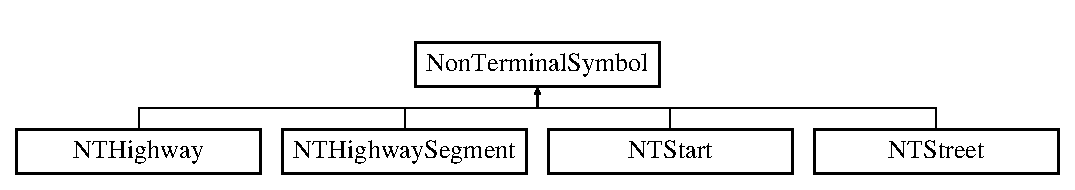
\includegraphics[height=2.000000cm]{class_non_terminal_symbol}
\end{center}
\end{figure}
\subsection*{Public Member Functions}
\begin{DoxyCompactItemize}
\item 
virtual \hyperlink{class_non_terminal_symbol}{Non\+Terminal\+Symbol} $\ast$ \hyperlink{class_non_terminal_symbol_ade38f1475002e4f8b41e23d9c787e5e0}{replace} ()=0
\begin{DoxyCompactList}\small\item\em Creates new sub-\/generation of the L-\/\+System. \end{DoxyCompactList}\item 
void \hyperlink{class_non_terminal_symbol_a5836ba5450850843721742e40064c5dc}{insert\+Sublist} (\hyperlink{class_non_terminal_symbol}{Non\+Terminal\+Symbol} $\ast$sublist, \hyperlink{class_non_terminal_symbol}{Non\+Terminal\+Symbol} $\ast$after)
\begin{DoxyCompactList}\small\item\em Inserts a sublist of N\+T-\/\+Elements. \end{DoxyCompactList}\end{DoxyCompactItemize}
\subsection*{Public Attributes}
\begin{DoxyCompactItemize}
\item 
\hypertarget{class_non_terminal_symbol_afd45d7cf8c469a93dee6d1683162a78a}{}\label{class_non_terminal_symbol_afd45d7cf8c469a93dee6d1683162a78a} 
bool \hyperlink{class_non_terminal_symbol_afd45d7cf8c469a93dee6d1683162a78a}{terminated\+\_\+}
\begin{DoxyCompactList}\small\item\em True until symbol can no longer be replaced (Termintates) \end{DoxyCompactList}\item 
\hypertarget{class_non_terminal_symbol_a378de10e3a1b73efc005d1f86dc8dd3e}{}\label{class_non_terminal_symbol_a378de10e3a1b73efc005d1f86dc8dd3e} 
\hyperlink{class_non_terminal_symbol}{Non\+Terminal\+Symbol} $\ast$ {\bfseries next\+\_\+}
\item 
\hypertarget{class_non_terminal_symbol_a1365061b52c674fbbcfe7178584ce65e}{}\label{class_non_terminal_symbol_a1365061b52c674fbbcfe7178584ce65e} 
\hyperlink{class_non_terminal_symbol}{Non\+Terminal\+Symbol} $\ast$ {\bfseries pre\+\_\+}
\end{DoxyCompactItemize}


\subsection{Detailed Description}
Parent class for all non-\/terminal members. 

Parent class of all the {\bfseries non-\/terminal} symbols that will be used by the grammar of our L-\/\+System. Every Non-\/\+Terminal symbol has a replace method that replaces it in the linked list (represented by the next\+\_\+ pointers) with its child elements -\/$>$ what the nonterminal turns into.

\begin{DoxyNote}{Note}
No Terminal class exists as N\+T-\/\+Members terminate based on a flag inside
\end{DoxyNote}
\begin{DoxyAuthor}{Author}
Lukas Gregori 
\end{DoxyAuthor}
\begin{DoxyVersion}{Version}

\end{DoxyVersion}
\begin{DoxyParagraph}{Revision}
1.\+0 
\end{DoxyParagraph}


Contact\+: \href{mailto:lukas.gregori@student.tugraz.at}{\tt lukas.\+gregori@student.\+tugraz.\+at}



 Copyright (C) Lukas Gregori, \href{mailto:contact@lukasgregori.com}{\tt contact@lukasgregori.\+com}

This file is part of the road network generator Road\+Gen.

Road\+Gen is free software\+: you can redistribute it and/or modify it under the terms of the G\+NU General Public License as published by the Free Software Foundation, either version 3 of the License, or (at your option) any later version.

Road\+Gen is distributed in the hope that it will be useful, but W\+I\+T\+H\+O\+UT A\+NY W\+A\+R\+R\+A\+N\+TY; without even the implied warranty of M\+E\+R\+C\+H\+A\+N\+T\+A\+B\+I\+L\+I\+TY or F\+I\+T\+N\+E\+SS F\+OR A P\+A\+R\+T\+I\+C\+U\+L\+AR P\+U\+R\+P\+O\+SE. See the G\+NU General Public License for more details.

You should have received a copy of the G\+NU General Public License \subsubsection*{along with Foobar. If not, see \href{http://www.gnu.org/licenses/}{\tt http\+://www.\+gnu.\+org/licenses/}. }

\subsection{Member Function Documentation}
\hypertarget{class_non_terminal_symbol_a5836ba5450850843721742e40064c5dc}{}\label{class_non_terminal_symbol_a5836ba5450850843721742e40064c5dc} 
\index{Non\+Terminal\+Symbol@{Non\+Terminal\+Symbol}!insert\+Sublist@{insert\+Sublist}}
\index{insert\+Sublist@{insert\+Sublist}!Non\+Terminal\+Symbol@{Non\+Terminal\+Symbol}}
\subsubsection{\texorpdfstring{insert\+Sublist()}{insertSublist()}}
{\footnotesize\ttfamily void Non\+Terminal\+Symbol\+::insert\+Sublist (\begin{DoxyParamCaption}\item[{\hyperlink{class_non_terminal_symbol}{Non\+Terminal\+Symbol} $\ast$}]{sublist,  }\item[{\hyperlink{class_non_terminal_symbol}{Non\+Terminal\+Symbol} $\ast$}]{after }\end{DoxyParamCaption})}



Inserts a sublist of N\+T-\/\+Elements. 

Inserts a sublist of elements handed as parameter into a second list specified by the after parameter. Used as each segment replaces itself in the list


\begin{DoxyParams}{Parameters}
{\em Non\+Terminal\+Symbol$\ast$} & sublist Sublist to insert \\
\hline
{\em Non\+Terminal\+Symbol$\ast$} & after Insert after this element \\
\hline
\end{DoxyParams}
\hypertarget{class_non_terminal_symbol_ade38f1475002e4f8b41e23d9c787e5e0}{}\label{class_non_terminal_symbol_ade38f1475002e4f8b41e23d9c787e5e0} 
\index{Non\+Terminal\+Symbol@{Non\+Terminal\+Symbol}!replace@{replace}}
\index{replace@{replace}!Non\+Terminal\+Symbol@{Non\+Terminal\+Symbol}}
\subsubsection{\texorpdfstring{replace()}{replace()}}
{\footnotesize\ttfamily virtual \hyperlink{class_non_terminal_symbol}{Non\+Terminal\+Symbol}$\ast$ Non\+Terminal\+Symbol\+::replace (\begin{DoxyParamCaption}{ }\end{DoxyParamCaption})\hspace{0.3cm}{\ttfamily [pure virtual]}}



Creates new sub-\/generation of the L-\/\+System. 

Replaces the non-\/terminal symbol by its successors. Returns the object itself so that it can be freed afterwards.

\begin{DoxyReturn}{Returns}
Non\+Terminal\+Symbol$\ast$ self 
\end{DoxyReturn}


Implemented in \hyperlink{class_n_t_street_ac3aa05ca530c99b178a855fc736b1a76}{N\+T\+Street}, \hyperlink{class_n_t_highway_segment_a22518e50d87a70aeb1ead58b26dfa483}{N\+T\+Highway\+Segment}, \hyperlink{class_n_t_start_a3f9897b293a26b301415a9089b90697b}{N\+T\+Start}, and \hyperlink{class_n_t_highway_a5a33cf5f76b36a1d62685408306a54c9}{N\+T\+Highway}.



The documentation for this class was generated from the following files\+:\begin{DoxyCompactItemize}
\item 
C\+:/\+Users/lukas/\+Desktop/\+Road\+Gen\+L\+Systems/Non\+Terminal\+Symbol.\+h\item 
C\+:/\+Users/lukas/\+Desktop/\+Road\+Gen\+L\+Systems/Non\+Terminal\+Symbol.\+cpp\end{DoxyCompactItemize}

\hypertarget{class_n_t_highway}{}\section{N\+T\+Highway Class Reference}
\label{class_n_t_highway}\index{N\+T\+Highway@{N\+T\+Highway}}


Start for the highway creation.  




{\ttfamily \#include $<$N\+T\+Highway.\+h$>$}

Inheritance diagram for N\+T\+Highway\+:\begin{figure}[H]
\begin{center}
\leavevmode
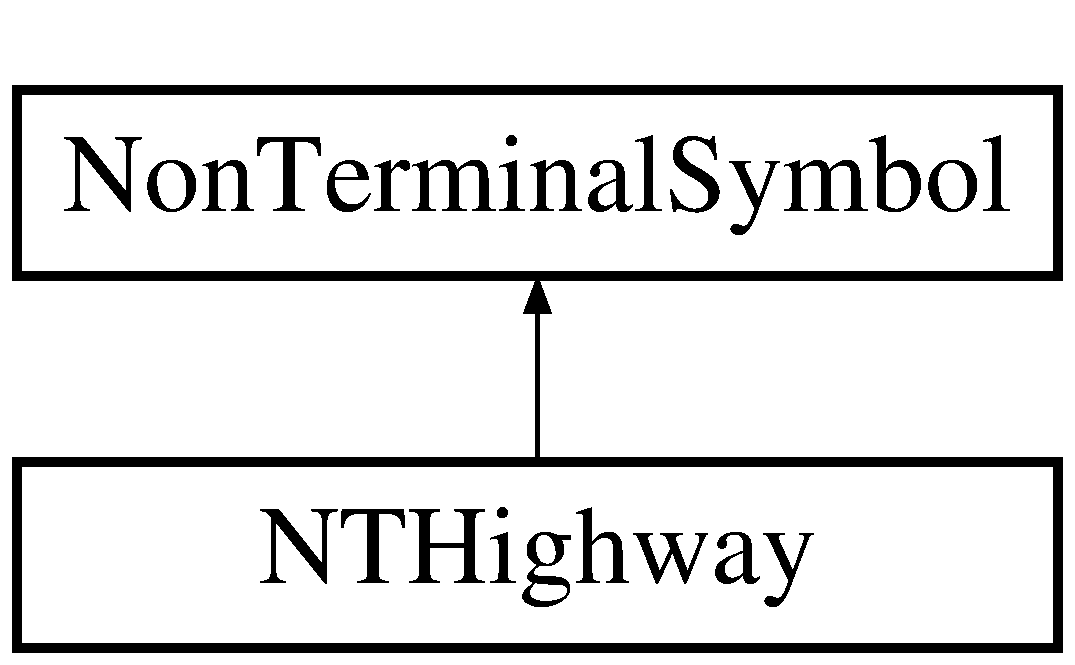
\includegraphics[height=2.000000cm]{class_n_t_highway}
\end{center}
\end{figure}
\subsection*{Public Member Functions}
\begin{DoxyCompactItemize}
\item 
\hypertarget{class_n_t_highway_aa71c2a81df557af649ed3a0562615526}{}\label{class_n_t_highway_aa71c2a81df557af649ed3a0562615526} 
{\bfseries N\+T\+Highway} (C\+G\+A\+L\+::\+M\+P\+\_\+\+Float x, C\+G\+A\+L\+::\+M\+P\+\_\+\+Float y, std\+::vector$<$ Point\+\_\+2 $>$ $\ast$high\+\_\+dens\+\_\+points)
\item 
\hyperlink{class_non_terminal_symbol}{Non\+Terminal\+Symbol} $\ast$ \hyperlink{class_n_t_highway_a5a33cf5f76b36a1d62685408306a54c9}{replace} ()
\begin{DoxyCompactList}\small\item\em Creates new sub-\/generation of the L-\/\+System. \end{DoxyCompactList}\end{DoxyCompactItemize}
\subsection*{Additional Inherited Members}


\subsection{Detailed Description}
Start for the highway creation. 

Wrapper rule for the actual highway segments (\hyperlink{class_n_t_highway_segment}{N\+T\+Highway\+Segment}). Creates as many segments as high density points gotten by the constructor

\begin{DoxyAuthor}{Author}
Lukas Gregori 
\end{DoxyAuthor}
\begin{DoxyVersion}{Version}

\end{DoxyVersion}
\begin{DoxyParagraph}{Revision}
1.\+0 
\end{DoxyParagraph}


Contact\+: \href{mailto:lukas.gregori@student.tugraz.at}{\tt lukas.\+gregori@student.\+tugraz.\+at}



 Copyright (C) Lukas Gregori, \href{mailto:contact@lukasgregori.com}{\tt contact@lukasgregori.\+com}

This file is part of the road network generator Road\+Gen.

Road\+Gen is free software\+: you can redistribute it and/or modify it under the terms of the G\+NU General Public License as published by the Free Software Foundation, either version 3 of the License, or (at your option) any later version.

Road\+Gen is distributed in the hope that it will be useful, but W\+I\+T\+H\+O\+UT A\+NY W\+A\+R\+R\+A\+N\+TY; without even the implied warranty of M\+E\+R\+C\+H\+A\+N\+T\+A\+B\+I\+L\+I\+TY or F\+I\+T\+N\+E\+SS F\+OR A P\+A\+R\+T\+I\+C\+U\+L\+AR P\+U\+R\+P\+O\+SE. See the G\+NU General Public License for more details.

You should have received a copy of the G\+NU General Public License \subsubsection*{along with Foobar. If not, see \href{http://www.gnu.org/licenses/}{\tt http\+://www.\+gnu.\+org/licenses/}. }

\subsection{Member Function Documentation}
\hypertarget{class_n_t_highway_a5a33cf5f76b36a1d62685408306a54c9}{}\label{class_n_t_highway_a5a33cf5f76b36a1d62685408306a54c9} 
\index{N\+T\+Highway@{N\+T\+Highway}!replace@{replace}}
\index{replace@{replace}!N\+T\+Highway@{N\+T\+Highway}}
\subsubsection{\texorpdfstring{replace()}{replace()}}
{\footnotesize\ttfamily \hyperlink{class_non_terminal_symbol}{Non\+Terminal\+Symbol} $\ast$ N\+T\+Highway\+::replace (\begin{DoxyParamCaption}{ }\end{DoxyParamCaption})\hspace{0.3cm}{\ttfamily [virtual]}}



Creates new sub-\/generation of the L-\/\+System. 

Replaces the non-\/terminal symbol by its successors. Returns the object itself so that it can be freed afterwards.

\begin{DoxyReturn}{Returns}
Non\+Terminal\+Symbol$\ast$ self 
\end{DoxyReturn}


Implements \hyperlink{class_non_terminal_symbol_ade38f1475002e4f8b41e23d9c787e5e0}{Non\+Terminal\+Symbol}.



The documentation for this class was generated from the following files\+:\begin{DoxyCompactItemize}
\item 
C\+:/\+Users/lukas/\+Desktop/\+Road\+Gen\+L\+Systems/N\+T\+Highway.\+h\item 
C\+:/\+Users/lukas/\+Desktop/\+Road\+Gen\+L\+Systems/N\+T\+Highway.\+cpp\end{DoxyCompactItemize}

\hypertarget{class_n_t_highway_segment}{}\section{N\+T\+Highway\+Segment Class Reference}
\label{class_n_t_highway_segment}\index{N\+T\+Highway\+Segment@{N\+T\+Highway\+Segment}}


Smallest unit of highway.  




{\ttfamily \#include $<$N\+T\+Highway\+Segment.\+h$>$}

Inheritance diagram for N\+T\+Highway\+Segment\+:\begin{figure}[H]
\begin{center}
\leavevmode
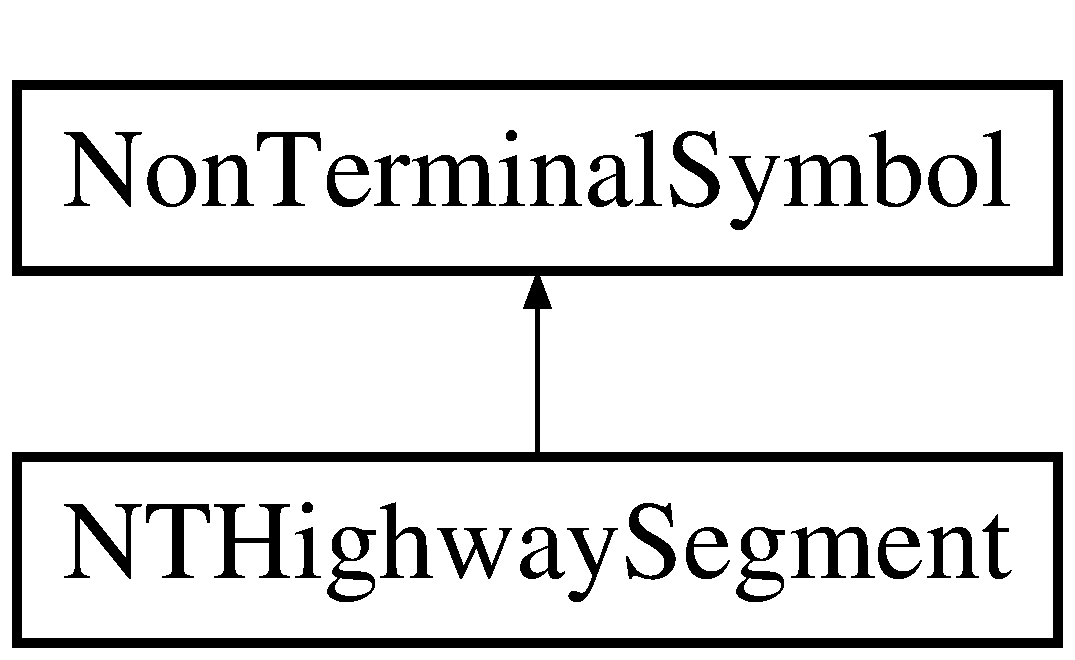
\includegraphics[height=2.000000cm]{class_n_t_highway_segment}
\end{center}
\end{figure}
\subsection*{Public Member Functions}
\begin{DoxyCompactItemize}
\item 
\hypertarget{class_n_t_highway_segment_adca391b80753f8fe54ab86657b9a49b6}{}\label{class_n_t_highway_segment_adca391b80753f8fe54ab86657b9a49b6} 
{\bfseries N\+T\+Highway\+Segment} (C\+G\+A\+L\+::\+M\+P\+\_\+\+Float x, C\+G\+A\+L\+::\+M\+P\+\_\+\+Float y, C\+G\+A\+L\+::\+M\+P\+\_\+\+Float x\+\_\+old, C\+G\+A\+L\+::\+M\+P\+\_\+\+Float y\+\_\+old, unsigned total\+\_\+distance, Point\+\_\+2 goal, bool create\+\_\+street)
\item 
\hyperlink{class_non_terminal_symbol}{Non\+Terminal\+Symbol} $\ast$ \hyperlink{class_n_t_highway_segment_a22518e50d87a70aeb1ead58b26dfa483}{replace} ()
\begin{DoxyCompactList}\small\item\em Creates new sub-\/generation of the L-\/\+System. \end{DoxyCompactList}\item 
void \hyperlink{class_n_t_highway_segment_a0008e99793162c8d78903aa9d35518df}{handle\+River\+Intersection} (Point\+\_\+2 closest\+\_\+intersection, Point\+\_\+2 farther\+\_\+intersection, Point\+\_\+2 old\+\_\+position)
\begin{DoxyCompactList}\small\item\em Handles intersections of highway segments with rivers. \end{DoxyCompactList}\item 
bool \hyperlink{class_n_t_highway_segment_adad0b1eecee26cfb43a6f53bbf560a1c}{check\+For\+River\+Intersection} (vector$<$ Point\+\_\+2 $>$ river\+\_\+intersections, Point\+\_\+2 new\+\_\+position, Point\+\_\+2 old\+\_\+position)
\begin{DoxyCompactList}\small\item\em Checks if there are intersections with a river and if so handles them accordingly. \end{DoxyCompactList}\end{DoxyCompactItemize}
\subsection*{Additional Inherited Members}


\subsection{Detailed Description}
Smallest unit of highway. 

The segments that make up the actual highway. Highways always grow towards a certain goal point (high density point in this case).

\begin{DoxyAuthor}{Author}
Lukas Gregori 
\end{DoxyAuthor}
\begin{DoxyVersion}{Version}

\end{DoxyVersion}
\begin{DoxyParagraph}{Revision}
1.\+0 
\end{DoxyParagraph}


Contact\+: \href{mailto:lukas.gregori@student.tugraz.at}{\tt lukas.\+gregori@student.\+tugraz.\+at}



 Copyright (C) Lukas Gregori, \href{mailto:contact@lukasgregori.com}{\tt contact@lukasgregori.\+com}

This file is part of the road network generator Road\+Gen.

Road\+Gen is free software\+: you can redistribute it and/or modify it under the terms of the G\+NU General Public License as published by the Free Software Foundation, either version 3 of the License, or (at your option) any later version.

Road\+Gen is distributed in the hope that it will be useful, but W\+I\+T\+H\+O\+UT A\+NY W\+A\+R\+R\+A\+N\+TY; without even the implied warranty of M\+E\+R\+C\+H\+A\+N\+T\+A\+B\+I\+L\+I\+TY or F\+I\+T\+N\+E\+SS F\+OR A P\+A\+R\+T\+I\+C\+U\+L\+AR P\+U\+R\+P\+O\+SE. See the G\+NU General Public License for more details.

You should have received a copy of the G\+NU General Public License \subsubsection*{along with Foobar. If not, see \href{http://www.gnu.org/licenses/}{\tt http\+://www.\+gnu.\+org/licenses/}. }

\subsection{Member Function Documentation}
\hypertarget{class_n_t_highway_segment_adad0b1eecee26cfb43a6f53bbf560a1c}{}\label{class_n_t_highway_segment_adad0b1eecee26cfb43a6f53bbf560a1c} 
\index{N\+T\+Highway\+Segment@{N\+T\+Highway\+Segment}!check\+For\+River\+Intersection@{check\+For\+River\+Intersection}}
\index{check\+For\+River\+Intersection@{check\+For\+River\+Intersection}!N\+T\+Highway\+Segment@{N\+T\+Highway\+Segment}}
\subsubsection{\texorpdfstring{check\+For\+River\+Intersection()}{checkForRiverIntersection()}}
{\footnotesize\ttfamily bool N\+T\+Highway\+Segment\+::check\+For\+River\+Intersection (\begin{DoxyParamCaption}\item[{vector$<$ Point\+\_\+2 $>$}]{river\+\_\+intersections,  }\item[{Point\+\_\+2}]{new\+\_\+position,  }\item[{Point\+\_\+2}]{old\+\_\+position }\end{DoxyParamCaption})}



Checks if there are intersections with a river and if so handles them accordingly. 

Checks if there are intersections of a highway segment with a river. If this is the case, the segment has to be handled accordingly (Call handle\+Rier\+Intersection method).


\begin{DoxyParams}{Parameters}
{\em vector$<$\+Point\+\_\+2$>$} & river\+\_\+intersections Contains possible intersections \\
\hline
{\em Point\+\_\+2} & new\+\_\+position Old end position before conlission \\
\hline
{\em Point\+\_\+2} & old\+\_\+position Old start position before conlission \\
\hline
\end{DoxyParams}
\hypertarget{class_n_t_highway_segment_a0008e99793162c8d78903aa9d35518df}{}\label{class_n_t_highway_segment_a0008e99793162c8d78903aa9d35518df} 
\index{N\+T\+Highway\+Segment@{N\+T\+Highway\+Segment}!handle\+River\+Intersection@{handle\+River\+Intersection}}
\index{handle\+River\+Intersection@{handle\+River\+Intersection}!N\+T\+Highway\+Segment@{N\+T\+Highway\+Segment}}
\subsubsection{\texorpdfstring{handle\+River\+Intersection()}{handleRiverIntersection()}}
{\footnotesize\ttfamily void N\+T\+Highway\+Segment\+::handle\+River\+Intersection (\begin{DoxyParamCaption}\item[{Point\+\_\+2}]{closest\+\_\+intersection,  }\item[{Point\+\_\+2}]{farther\+\_\+intersection,  }\item[{Point\+\_\+2}]{old\+\_\+position }\end{DoxyParamCaption})}



Handles intersections of highway segments with rivers. 

If a highway intersects with a river, the segment is extended further to reach the other side of the river. The two opposite points can now be connected with a bridge

At the other side of the river a new segment is created that can grow further (thus rivers do not automatically terminate highways).


\begin{DoxyParams}{Parameters}
{\em Point\+\_\+2} & closest\+\_\+intersection First conflict point \\
\hline
{\em Point\+\_\+2} & farther\+\_\+intersection Second conflict point got by extension \\
\hline
{\em Point\+\_\+2} & old\+\_\+position Old start position before conlission \\
\hline
\end{DoxyParams}
\hypertarget{class_n_t_highway_segment_a22518e50d87a70aeb1ead58b26dfa483}{}\label{class_n_t_highway_segment_a22518e50d87a70aeb1ead58b26dfa483} 
\index{N\+T\+Highway\+Segment@{N\+T\+Highway\+Segment}!replace@{replace}}
\index{replace@{replace}!N\+T\+Highway\+Segment@{N\+T\+Highway\+Segment}}
\subsubsection{\texorpdfstring{replace()}{replace()}}
{\footnotesize\ttfamily \hyperlink{class_non_terminal_symbol}{Non\+Terminal\+Symbol} $\ast$ N\+T\+Highway\+Segment\+::replace (\begin{DoxyParamCaption}{ }\end{DoxyParamCaption})\hspace{0.3cm}{\ttfamily [virtual]}}



Creates new sub-\/generation of the L-\/\+System. 

Replaces the non-\/terminal symbol by its successors. Returns the object itself so that it can be freed afterwards.

\begin{DoxyReturn}{Returns}
Non\+Terminal\+Symbol$\ast$ self 
\end{DoxyReturn}


Implements \hyperlink{class_non_terminal_symbol_ade38f1475002e4f8b41e23d9c787e5e0}{Non\+Terminal\+Symbol}.



The documentation for this class was generated from the following files\+:\begin{DoxyCompactItemize}
\item 
C\+:/\+Users/lukas/\+Desktop/\+Road\+Gen\+L\+Systems/N\+T\+Highway\+Segment.\+h\item 
C\+:/\+Users/lukas/\+Desktop/\+Road\+Gen\+L\+Systems/N\+T\+Highway\+Segment.\+cpp\end{DoxyCompactItemize}

\hypertarget{class_n_t_start}{}\section{N\+T\+Start Class Reference}
\label{class_n_t_start}\index{N\+T\+Start@{N\+T\+Start}}


Start point of the overall creation.  




{\ttfamily \#include $<$N\+T\+Start.\+h$>$}

Inheritance diagram for N\+T\+Start\+:\begin{figure}[H]
\begin{center}
\leavevmode
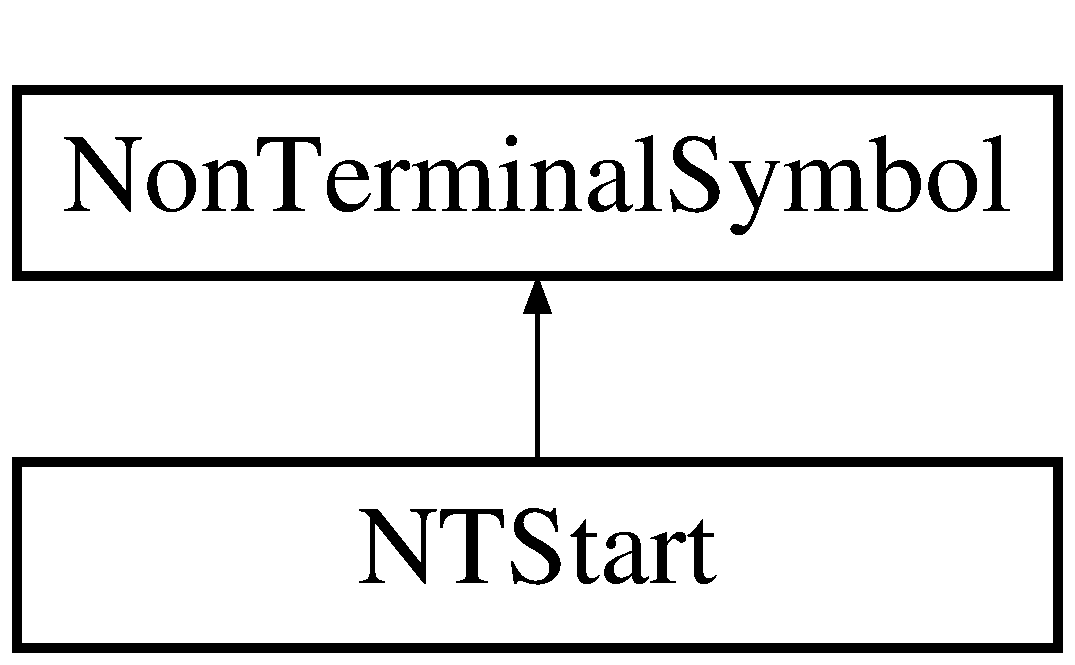
\includegraphics[height=2.000000cm]{class_n_t_start}
\end{center}
\end{figure}
\subsection*{Public Member Functions}
\begin{DoxyCompactItemize}
\item 
\hypertarget{class_n_t_start_a6b76194e7dddaea8bea60781cd288a7e}{}\label{class_n_t_start_a6b76194e7dddaea8bea60781cd288a7e} 
{\bfseries N\+T\+Start} (std\+::vector$<$ Point\+\_\+2 $>$ $\ast$high\+\_\+dens\+\_\+points, std\+::vector$<$ Point\+\_\+2 $>$ $\ast$start\+\_\+points)
\item 
\hyperlink{class_non_terminal_symbol}{Non\+Terminal\+Symbol} $\ast$ \hyperlink{class_n_t_start_a3f9897b293a26b301415a9089b90697b}{replace} ()
\begin{DoxyCompactList}\small\item\em Creates new sub-\/generation of the L-\/\+System. \end{DoxyCompactList}\end{DoxyCompactItemize}
\subsection*{Additional Inherited Members}


\subsection{Detailed Description}
Start point of the overall creation. 

Class \hyperlink{class_n_t_start}{N\+T\+Start}

\begin{DoxyNote}{Note}
Only one start point
\end{DoxyNote}
\begin{DoxyAuthor}{Author}
Lukas Gregori 
\end{DoxyAuthor}
\begin{DoxyVersion}{Version}

\end{DoxyVersion}
\begin{DoxyParagraph}{Revision}
1.\+0 
\end{DoxyParagraph}


Contact\+: \href{mailto:lukas.gregori@student.tugraz.at}{\tt lukas.\+gregori@student.\+tugraz.\+at}

Class implemented as singleton



 Copyright (C) Lukas Gregori, \href{mailto:contact@lukasgregori.com}{\tt contact@lukasgregori.\+com}

This file is part of the road network generator Road\+Gen.

Road\+Gen is free software\+: you can redistribute it and/or modify it under the terms of the G\+NU General Public License as published by the Free Software Foundation, either version 3 of the License, or (at your option) any later version.

Road\+Gen is distributed in the hope that it will be useful, but W\+I\+T\+H\+O\+UT A\+NY W\+A\+R\+R\+A\+N\+TY; without even the implied warranty of M\+E\+R\+C\+H\+A\+N\+T\+A\+B\+I\+L\+I\+TY or F\+I\+T\+N\+E\+SS F\+OR A P\+A\+R\+T\+I\+C\+U\+L\+AR P\+U\+R\+P\+O\+SE. See the G\+NU General Public License for more details.

You should have received a copy of the G\+NU General Public License \subsubsection*{along with Foobar. If not, see \href{http://www.gnu.org/licenses/}{\tt http\+://www.\+gnu.\+org/licenses/}. }

\subsection{Member Function Documentation}
\hypertarget{class_n_t_start_a3f9897b293a26b301415a9089b90697b}{}\label{class_n_t_start_a3f9897b293a26b301415a9089b90697b} 
\index{N\+T\+Start@{N\+T\+Start}!replace@{replace}}
\index{replace@{replace}!N\+T\+Start@{N\+T\+Start}}
\subsubsection{\texorpdfstring{replace()}{replace()}}
{\footnotesize\ttfamily \hyperlink{class_non_terminal_symbol}{Non\+Terminal\+Symbol} $\ast$ N\+T\+Start\+::replace (\begin{DoxyParamCaption}{ }\end{DoxyParamCaption})\hspace{0.3cm}{\ttfamily [virtual]}}



Creates new sub-\/generation of the L-\/\+System. 

Replaces the non-\/terminal symbol by its successors. Returns the object itself so that it can be freed afterwards.

\begin{DoxyReturn}{Returns}
Non\+Terminal\+Symbol$\ast$ self 
\end{DoxyReturn}


Implements \hyperlink{class_non_terminal_symbol_ade38f1475002e4f8b41e23d9c787e5e0}{Non\+Terminal\+Symbol}.



The documentation for this class was generated from the following files\+:\begin{DoxyCompactItemize}
\item 
C\+:/\+Users/lukas/\+Desktop/\+Road\+Gen\+L\+Systems/N\+T\+Start.\+h\item 
C\+:/\+Users/lukas/\+Desktop/\+Road\+Gen\+L\+Systems/N\+T\+Start.\+cpp\end{DoxyCompactItemize}

\hypertarget{class_n_t_street}{}\section{N\+T\+Street Class Reference}
\label{class_n_t_street}\index{N\+T\+Street@{N\+T\+Street}}


Smalles unit of street.  




{\ttfamily \#include $<$N\+T\+Street.\+h$>$}

Inheritance diagram for N\+T\+Street\+:\begin{figure}[H]
\begin{center}
\leavevmode
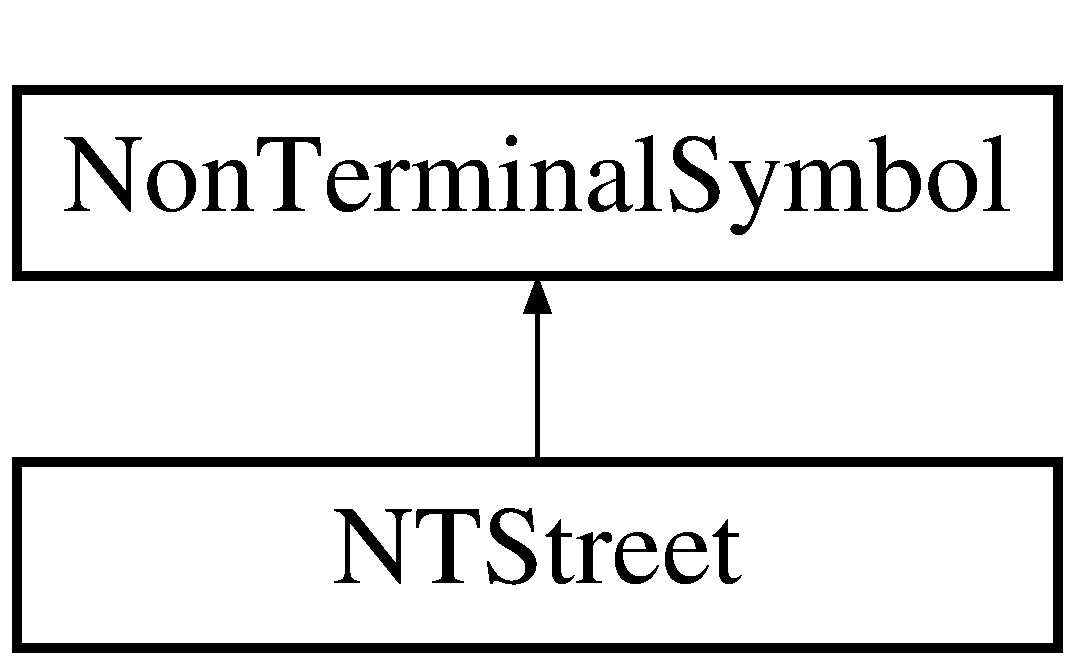
\includegraphics[height=2.000000cm]{class_n_t_street}
\end{center}
\end{figure}
\subsection*{Public Member Functions}
\begin{DoxyCompactItemize}
\item 
\hypertarget{class_n_t_street_aa0f2f63631f1cceea765e1c19f6180d6}{}\label{class_n_t_street_aa0f2f63631f1cceea765e1c19f6180d6} 
{\bfseries N\+T\+Street} (C\+G\+A\+L\+::\+M\+P\+\_\+\+Float x, C\+G\+A\+L\+::\+M\+P\+\_\+\+Float y, C\+G\+A\+L\+::\+M\+P\+\_\+\+Float x\+\_\+old, C\+G\+A\+L\+::\+M\+P\+\_\+\+Float y\+\_\+old)
\item 
\hyperlink{class_non_terminal_symbol}{Non\+Terminal\+Symbol} $\ast$ \hyperlink{class_n_t_street_ac3aa05ca530c99b178a855fc736b1a76}{replace} ()
\begin{DoxyCompactList}\small\item\em Creates new sub-\/generation of the L-\/\+System. \end{DoxyCompactList}\end{DoxyCompactItemize}
\subsection*{Additional Inherited Members}


\subsection{Detailed Description}
Smalles unit of street. 

Class \hyperlink{class_n_t_street}{N\+T\+Street}

Class used for handling the streets. Each street grows outwards with no specific goal (unlike the highways). The streets only keep the previous angle in mind (Do not want to steep angles of streets, should look natural).

Streets terminate at collision with any other media (including rivers), and branch based on a predefined probability (See C\+G\+A\+L\+Defs File).

\begin{DoxyNote}{Note}
No street segment subclass exists as with highways 

Streets have no target they grow to 

Terminate at collission 

Also terminate at river contact, no bridges
\end{DoxyNote}
\begin{DoxyAuthor}{Author}
Lukas Gregori 
\end{DoxyAuthor}
\begin{DoxyVersion}{Version}

\end{DoxyVersion}
\begin{DoxyParagraph}{Revision}
1.\+0 
\end{DoxyParagraph}


Contact\+: \href{mailto:lukas.gregori@student.tugraz.at}{\tt lukas.\+gregori@student.\+tugraz.\+at}



 Copyright (C) Lukas Gregori, \href{mailto:contact@lukasgregori.com}{\tt contact@lukasgregori.\+com}

This file is part of the road network generator Road\+Gen.

Road\+Gen is free software\+: you can redistribute it and/or modify it under the terms of the G\+NU General Public License as published by the Free Software Foundation, either version 3 of the License, or (at your option) any later version.

Road\+Gen is distributed in the hope that it will be useful, but W\+I\+T\+H\+O\+UT A\+NY W\+A\+R\+R\+A\+N\+TY; without even the implied warranty of M\+E\+R\+C\+H\+A\+N\+T\+A\+B\+I\+L\+I\+TY or F\+I\+T\+N\+E\+SS F\+OR A P\+A\+R\+T\+I\+C\+U\+L\+AR P\+U\+R\+P\+O\+SE. See the G\+NU General Public License for more details.

You should have received a copy of the G\+NU General Public License \subsubsection*{along with Foobar. If not, see \href{http://www.gnu.org/licenses/}{\tt http\+://www.\+gnu.\+org/licenses/}. }

\subsection{Member Function Documentation}
\hypertarget{class_n_t_street_ac3aa05ca530c99b178a855fc736b1a76}{}\label{class_n_t_street_ac3aa05ca530c99b178a855fc736b1a76} 
\index{N\+T\+Street@{N\+T\+Street}!replace@{replace}}
\index{replace@{replace}!N\+T\+Street@{N\+T\+Street}}
\subsubsection{\texorpdfstring{replace()}{replace()}}
{\footnotesize\ttfamily \hyperlink{class_non_terminal_symbol}{Non\+Terminal\+Symbol} $\ast$ N\+T\+Street\+::replace (\begin{DoxyParamCaption}{ }\end{DoxyParamCaption})\hspace{0.3cm}{\ttfamily [virtual]}}



Creates new sub-\/generation of the L-\/\+System. 

Replaces the non-\/terminal symbol by its successors. Returns the object itself so that it can be freed afterwards.

\begin{DoxyReturn}{Returns}
Non\+Terminal\+Symbol$\ast$ self 
\end{DoxyReturn}


Implements \hyperlink{class_non_terminal_symbol_ade38f1475002e4f8b41e23d9c787e5e0}{Non\+Terminal\+Symbol}.



The documentation for this class was generated from the following files\+:\begin{DoxyCompactItemize}
\item 
C\+:/\+Users/lukas/\+Desktop/\+Road\+Gen\+L\+Systems/N\+T\+Street.\+h\item 
C\+:/\+Users/lukas/\+Desktop/\+Road\+Gen\+L\+Systems/N\+T\+Street.\+cpp\end{DoxyCompactItemize}

\hypertarget{struct_clipper_lib_1_1_out_pt}{}\section{Clipper\+Lib\+:\+:Out\+Pt Struct Reference}
\label{struct_clipper_lib_1_1_out_pt}\index{Clipper\+Lib\+::\+Out\+Pt@{Clipper\+Lib\+::\+Out\+Pt}}
\subsection*{Public Attributes}
\begin{DoxyCompactItemize}
\item 
\hypertarget{struct_clipper_lib_1_1_out_pt_ad04d3691d47a5d0d9b2ae097e7e7bf10}{}\label{struct_clipper_lib_1_1_out_pt_ad04d3691d47a5d0d9b2ae097e7e7bf10} 
int {\bfseries Idx}
\item 
\hypertarget{struct_clipper_lib_1_1_out_pt_aa01c2b1e9c5b2d8faa40701178ffcf98}{}\label{struct_clipper_lib_1_1_out_pt_aa01c2b1e9c5b2d8faa40701178ffcf98} 
\hyperlink{struct_clipper_lib_1_1_int_point}{Int\+Point} {\bfseries Pt}
\item 
\hypertarget{struct_clipper_lib_1_1_out_pt_a2d605b87f6da37dbdbef990c4fa5819e}{}\label{struct_clipper_lib_1_1_out_pt_a2d605b87f6da37dbdbef990c4fa5819e} 
\hyperlink{struct_clipper_lib_1_1_out_pt}{Out\+Pt} $\ast$ {\bfseries Next}
\item 
\hypertarget{struct_clipper_lib_1_1_out_pt_a609eb414d5764e78150cceccaffc5d54}{}\label{struct_clipper_lib_1_1_out_pt_a609eb414d5764e78150cceccaffc5d54} 
\hyperlink{struct_clipper_lib_1_1_out_pt}{Out\+Pt} $\ast$ {\bfseries Prev}
\end{DoxyCompactItemize}


The documentation for this struct was generated from the following file\+:\begin{DoxyCompactItemize}
\item 
C\+:/\+Users/lukas/\+Desktop/\+Road\+Gen\+L\+Systems/Clipper.\+cpp\end{DoxyCompactItemize}

\hypertarget{struct_clipper_lib_1_1_out_rec}{}\section{Clipper\+Lib\+:\+:Out\+Rec Struct Reference}
\label{struct_clipper_lib_1_1_out_rec}\index{Clipper\+Lib\+::\+Out\+Rec@{Clipper\+Lib\+::\+Out\+Rec}}
\subsection*{Public Attributes}
\begin{DoxyCompactItemize}
\item 
\hypertarget{struct_clipper_lib_1_1_out_rec_ae2c437dec114034a456a7238ab6d8055}{}\label{struct_clipper_lib_1_1_out_rec_ae2c437dec114034a456a7238ab6d8055} 
int {\bfseries Idx}
\item 
\hypertarget{struct_clipper_lib_1_1_out_rec_a18b2b534b717139528047ba10a1c805c}{}\label{struct_clipper_lib_1_1_out_rec_a18b2b534b717139528047ba10a1c805c} 
bool {\bfseries Is\+Hole}
\item 
\hypertarget{struct_clipper_lib_1_1_out_rec_a065731c084453a818939c219868a2fcc}{}\label{struct_clipper_lib_1_1_out_rec_a065731c084453a818939c219868a2fcc} 
bool {\bfseries Is\+Open}
\item 
\hypertarget{struct_clipper_lib_1_1_out_rec_aa8baa934f1a7687a16b88a579dec3dd4}{}\label{struct_clipper_lib_1_1_out_rec_aa8baa934f1a7687a16b88a579dec3dd4} 
\hyperlink{struct_clipper_lib_1_1_out_rec}{Out\+Rec} $\ast$ {\bfseries First\+Left}
\item 
\hypertarget{struct_clipper_lib_1_1_out_rec_a334af720a9e0a815ba690e80e32bebd1}{}\label{struct_clipper_lib_1_1_out_rec_a334af720a9e0a815ba690e80e32bebd1} 
\hyperlink{class_clipper_lib_1_1_poly_node}{Poly\+Node} $\ast$ {\bfseries Poly\+Nd}
\item 
\hypertarget{struct_clipper_lib_1_1_out_rec_a82e9cba88d46d0d60db0b0365c6bd02e}{}\label{struct_clipper_lib_1_1_out_rec_a82e9cba88d46d0d60db0b0365c6bd02e} 
\hyperlink{struct_clipper_lib_1_1_out_pt}{Out\+Pt} $\ast$ {\bfseries Pts}
\item 
\hypertarget{struct_clipper_lib_1_1_out_rec_adc4d612df109de83dca298204176ff0c}{}\label{struct_clipper_lib_1_1_out_rec_adc4d612df109de83dca298204176ff0c} 
\hyperlink{struct_clipper_lib_1_1_out_pt}{Out\+Pt} $\ast$ {\bfseries Bottom\+Pt}
\end{DoxyCompactItemize}


The documentation for this struct was generated from the following file\+:\begin{DoxyCompactItemize}
\item 
C\+:/\+Users/lukas/\+Desktop/\+Road\+Gen\+L\+Systems/Clipper.\+cpp\end{DoxyCompactItemize}

\hypertarget{class_clipper_lib_1_1_poly_node}{}\section{Clipper\+Lib\+:\+:Poly\+Node Class Reference}
\label{class_clipper_lib_1_1_poly_node}\index{Clipper\+Lib\+::\+Poly\+Node@{Clipper\+Lib\+::\+Poly\+Node}}
Inheritance diagram for Clipper\+Lib\+:\+:Poly\+Node\+:\begin{figure}[H]
\begin{center}
\leavevmode
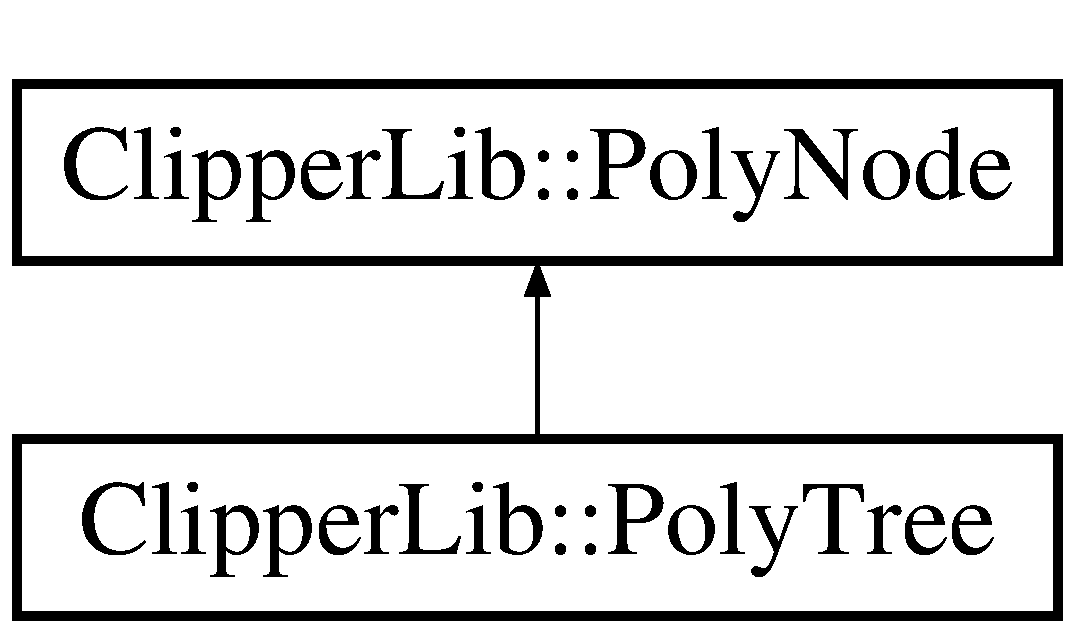
\includegraphics[height=2.000000cm]{class_clipper_lib_1_1_poly_node}
\end{center}
\end{figure}
\subsection*{Public Member Functions}
\begin{DoxyCompactItemize}
\item 
\hypertarget{class_clipper_lib_1_1_poly_node_adbcb861001d8bfbd609c4ba4f4a19a58}{}\label{class_clipper_lib_1_1_poly_node_adbcb861001d8bfbd609c4ba4f4a19a58} 
\hyperlink{class_clipper_lib_1_1_poly_node}{Poly\+Node} $\ast$ {\bfseries Get\+Next} () const
\item 
\hypertarget{class_clipper_lib_1_1_poly_node_a0467801cae1b28ad8a4917b96e551536}{}\label{class_clipper_lib_1_1_poly_node_a0467801cae1b28ad8a4917b96e551536} 
bool {\bfseries Is\+Hole} () const
\item 
\hypertarget{class_clipper_lib_1_1_poly_node_ac9ade640af2515976d337b65e8e84776}{}\label{class_clipper_lib_1_1_poly_node_ac9ade640af2515976d337b65e8e84776} 
bool {\bfseries Is\+Open} () const
\item 
\hypertarget{class_clipper_lib_1_1_poly_node_a19128db6fb2aca66555231edaffa7ade}{}\label{class_clipper_lib_1_1_poly_node_a19128db6fb2aca66555231edaffa7ade} 
int {\bfseries Child\+Count} () const
\end{DoxyCompactItemize}
\subsection*{Public Attributes}
\begin{DoxyCompactItemize}
\item 
\hypertarget{class_clipper_lib_1_1_poly_node_a1d08b8a9499ff8cb89d5d63a12f881ea}{}\label{class_clipper_lib_1_1_poly_node_a1d08b8a9499ff8cb89d5d63a12f881ea} 
Path {\bfseries Contour}
\item 
\hypertarget{class_clipper_lib_1_1_poly_node_a7ac59aea508951a4c979bfca8913261d}{}\label{class_clipper_lib_1_1_poly_node_a7ac59aea508951a4c979bfca8913261d} 
Poly\+Nodes {\bfseries Childs}
\item 
\hypertarget{class_clipper_lib_1_1_poly_node_a9465bc02623316de2af3ab52c6f7041e}{}\label{class_clipper_lib_1_1_poly_node_a9465bc02623316de2af3ab52c6f7041e} 
\hyperlink{class_clipper_lib_1_1_poly_node}{Poly\+Node} $\ast$ {\bfseries Parent}
\end{DoxyCompactItemize}
\subsection*{Friends}
\begin{DoxyCompactItemize}
\item 
\hypertarget{class_clipper_lib_1_1_poly_node_a4d39a09ecdddeeb85930dd4554a54b3c}{}\label{class_clipper_lib_1_1_poly_node_a4d39a09ecdddeeb85930dd4554a54b3c} 
class {\bfseries Clipper}
\item 
\hypertarget{class_clipper_lib_1_1_poly_node_adadfb8ac9a17a5c8fb7b4f012075b975}{}\label{class_clipper_lib_1_1_poly_node_adadfb8ac9a17a5c8fb7b4f012075b975} 
class {\bfseries Clipper\+Offset}
\end{DoxyCompactItemize}


The documentation for this class was generated from the following files\+:\begin{DoxyCompactItemize}
\item 
C\+:/\+Users/lukas/\+Desktop/\+Road\+Gen\+L\+Systems/Clipper.\+h\item 
C\+:/\+Users/lukas/\+Desktop/\+Road\+Gen\+L\+Systems/Clipper.\+cpp\end{DoxyCompactItemize}

\hypertarget{class_clipper_lib_1_1_poly_tree}{}\section{Clipper\+Lib\+:\+:Poly\+Tree Class Reference}
\label{class_clipper_lib_1_1_poly_tree}\index{Clipper\+Lib\+::\+Poly\+Tree@{Clipper\+Lib\+::\+Poly\+Tree}}
Inheritance diagram for Clipper\+Lib\+:\+:Poly\+Tree\+:\begin{figure}[H]
\begin{center}
\leavevmode
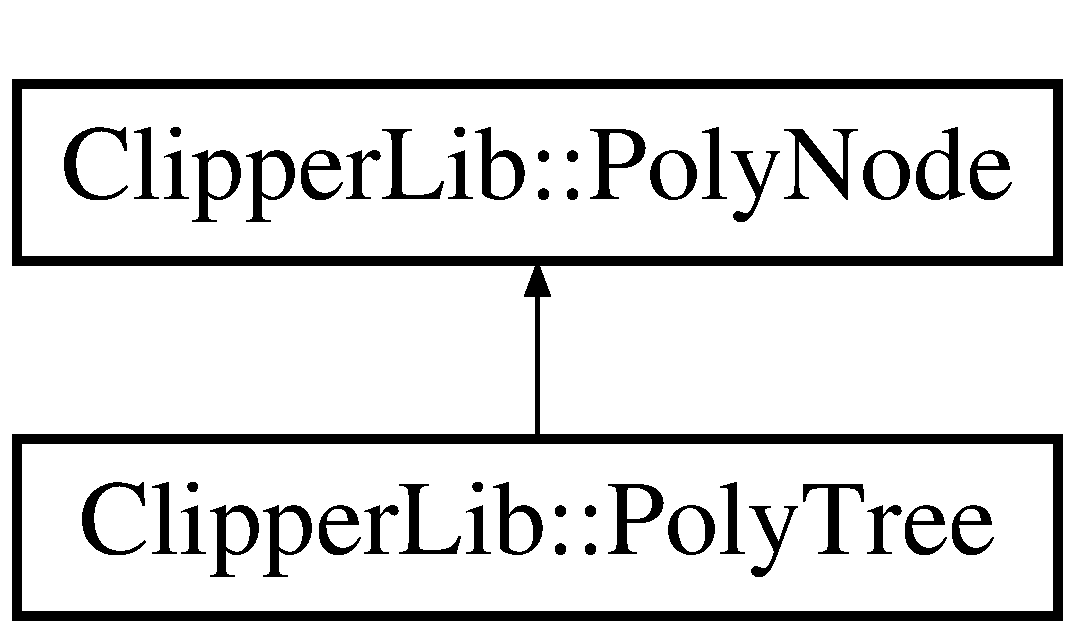
\includegraphics[height=2.000000cm]{class_clipper_lib_1_1_poly_tree}
\end{center}
\end{figure}
\subsection*{Public Member Functions}
\begin{DoxyCompactItemize}
\item 
\hypertarget{class_clipper_lib_1_1_poly_tree_a8b88b8d6225281ee7d536902b0d04e9e}{}\label{class_clipper_lib_1_1_poly_tree_a8b88b8d6225281ee7d536902b0d04e9e} 
\hyperlink{class_clipper_lib_1_1_poly_node}{Poly\+Node} $\ast$ {\bfseries Get\+First} () const
\item 
\hypertarget{class_clipper_lib_1_1_poly_tree_a8620ea631d478b3c43274ac084902ec4}{}\label{class_clipper_lib_1_1_poly_tree_a8620ea631d478b3c43274ac084902ec4} 
void {\bfseries Clear} ()
\item 
\hypertarget{class_clipper_lib_1_1_poly_tree_ad0d3c974bab5a30cc8c916da9fe14388}{}\label{class_clipper_lib_1_1_poly_tree_ad0d3c974bab5a30cc8c916da9fe14388} 
int {\bfseries Total} () const
\end{DoxyCompactItemize}
\subsection*{Friends}
\begin{DoxyCompactItemize}
\item 
\hypertarget{class_clipper_lib_1_1_poly_tree_a4d39a09ecdddeeb85930dd4554a54b3c}{}\label{class_clipper_lib_1_1_poly_tree_a4d39a09ecdddeeb85930dd4554a54b3c} 
class {\bfseries Clipper}
\end{DoxyCompactItemize}
\subsection*{Additional Inherited Members}


The documentation for this class was generated from the following files\+:\begin{DoxyCompactItemize}
\item 
C\+:/\+Users/lukas/\+Desktop/\+Road\+Gen\+L\+Systems/Clipper.\+h\item 
C\+:/\+Users/lukas/\+Desktop/\+Road\+Gen\+L\+Systems/Clipper.\+cpp\end{DoxyCompactItemize}

\hypertarget{class_post_script_int_writer}{}\section{Post\+Script\+Int\+Writer Class Reference}
\label{class_post_script_int_writer}\index{Post\+Script\+Int\+Writer@{Post\+Script\+Int\+Writer}}


Generates Output (.pst File) from generated information.  




{\ttfamily \#include $<$Post\+Script\+Int\+Writer.\+h$>$}

Inheritance diagram for Post\+Script\+Int\+Writer\+:\begin{figure}[H]
\begin{center}
\leavevmode
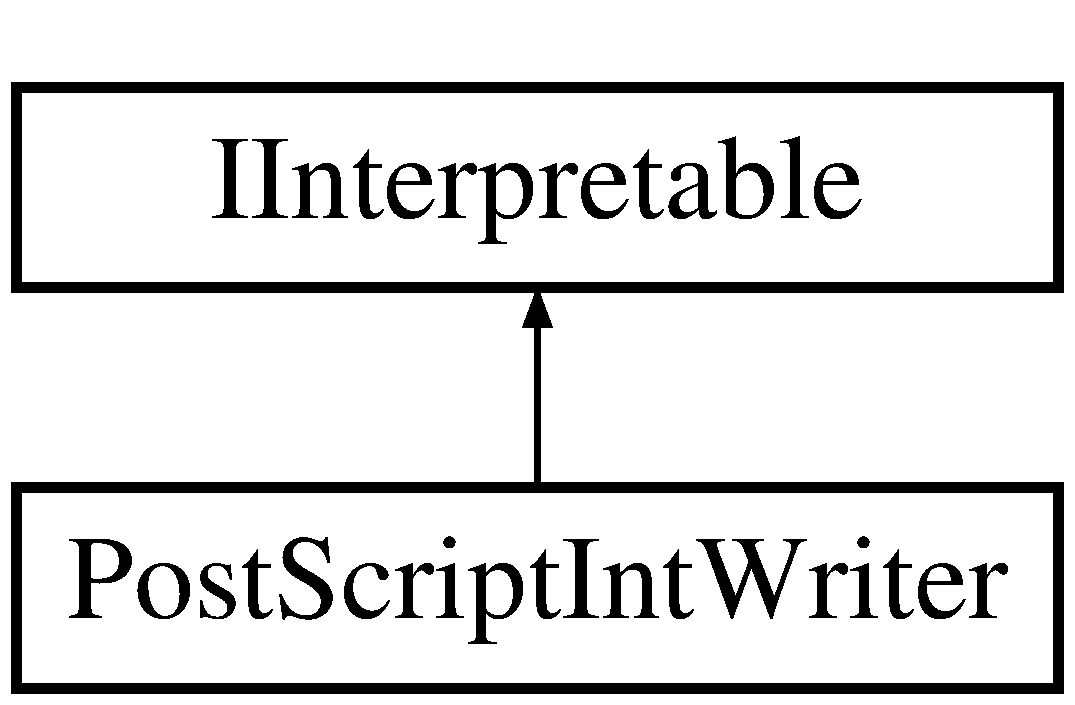
\includegraphics[height=2.000000cm]{class_post_script_int_writer}
\end{center}
\end{figure}
\subsection*{Public Member Functions}
\begin{DoxyCompactItemize}
\item 
\hypertarget{class_post_script_int_writer_a0cfdc6026b5a0067c97e0724b6d3f274}{}\label{class_post_script_int_writer_a0cfdc6026b5a0067c97e0724b6d3f274} 
void {\bfseries handle\+Interception} (C\+G\+A\+L\+::\+M\+P\+\_\+\+Float x, C\+G\+A\+L\+::\+M\+P\+\_\+\+Float y)
\item 
\hypertarget{class_post_script_int_writer_ac25b006a0eeaf2389e80b8f5ac4abea6}{}\label{class_post_script_int_writer_ac25b006a0eeaf2389e80b8f5ac4abea6} 
void {\bfseries handle\+Highway\+Interception} (C\+G\+A\+L\+::\+M\+P\+\_\+\+Float x, C\+G\+A\+L\+::\+M\+P\+\_\+\+Float y)
\item 
\hypertarget{class_post_script_int_writer_a01160610eeab71add25021437d6d4a6a}{}\label{class_post_script_int_writer_a01160610eeab71add25021437d6d4a6a} 
void {\bfseries handle\+High\+Density\+Point} (C\+G\+A\+L\+::\+M\+P\+\_\+\+Float x, C\+G\+A\+L\+::\+M\+P\+\_\+\+Float y, int max\+\_\+diameter)
\item 
\hypertarget{class_post_script_int_writer_a8727400a956271d23d8ba582bca30273}{}\label{class_post_script_int_writer_a8727400a956271d23d8ba582bca30273} 
void {\bfseries handle\+Street\+Segments} (vector$<$ Segment\+\_\+2 $>$ streets)
\item 
\hypertarget{class_post_script_int_writer_aea0d5736a30736b0aa6e8ebe7c903478}{}\label{class_post_script_int_writer_aea0d5736a30736b0aa6e8ebe7c903478} 
void {\bfseries handle\+Highway\+Segments} (vector$<$ Segment\+\_\+2 $>$ highways)
\item 
\hypertarget{class_post_script_int_writer_acb5dbf5b3e10b0ab3a8ab3c1a3e0e1e6}{}\label{class_post_script_int_writer_acb5dbf5b3e10b0ab3a8ab3c1a3e0e1e6} 
void {\bfseries handle\+River} (vector$<$ Segment\+\_\+2 $>$ river)
\item 
\hypertarget{class_post_script_int_writer_ac00aa8d3cbf17c94653ae31f4c91eff4}{}\label{class_post_script_int_writer_ac00aa8d3cbf17c94653ae31f4c91eff4} 
void {\bfseries handle\+Error} (vector$<$ Segment\+\_\+2 $>$ river)
\item 
\hypertarget{class_post_script_int_writer_ae763ce8b90fb0d2a79eae84e2f9be3a4}{}\label{class_post_script_int_writer_ae763ce8b90fb0d2a79eae84e2f9be3a4} 
void {\bfseries handle\+Bridges} (vector$<$ Segment\+\_\+2 $>$ bridges)
\item 
\hypertarget{class_post_script_int_writer_aab4c0b129676f0c120acd1888f3b3cac}{}\label{class_post_script_int_writer_aab4c0b129676f0c120acd1888f3b3cac} 
void {\bfseries handle\+Trees} (vector$<$ Point\+\_\+2 $>$ trees)
\item 
\hypertarget{class_post_script_int_writer_a9c563b05ac9aa1cca1d9f9f8318c676b}{}\label{class_post_script_int_writer_a9c563b05ac9aa1cca1d9f9f8318c676b} 
void {\bfseries handle\+Lights} (vector$<$ Point\+\_\+2 $>$ lights)
\item 
\hypertarget{class_post_script_int_writer_ab3b394c6e8e0f71bd9b4ac859ea961a7}{}\label{class_post_script_int_writer_ab3b394c6e8e0f71bd9b4ac859ea961a7} 
void {\bfseries handle\+New\+Highway\+Start} (C\+G\+A\+L\+::\+M\+P\+\_\+\+Float x, C\+G\+A\+L\+::\+M\+P\+\_\+\+Float y)
\item 
\hypertarget{class_post_script_int_writer_a33016680eb1388e3beab4bae0305e8a9}{}\label{class_post_script_int_writer_a33016680eb1388e3beab4bae0305e8a9} 
void {\bfseries handle\+Highway\+Exit} (C\+G\+A\+L\+::\+M\+P\+\_\+\+Float x, C\+G\+A\+L\+::\+M\+P\+\_\+\+Float y)
\item 
\hypertarget{class_post_script_int_writer_a042a255dc892a2b80936cbf29fb98583}{}\label{class_post_script_int_writer_a042a255dc892a2b80936cbf29fb98583} 
void {\bfseries start\+Network} ()
\item 
\hypertarget{class_post_script_int_writer_a89ab69da091fa23ceaf89088434fc336}{}\label{class_post_script_int_writer_a89ab69da091fa23ceaf89088434fc336} 
void {\bfseries close\+Network} ()
\item 
\hypertarget{class_post_script_int_writer_a7dbf0010930eec0d32dea5649543cc22}{}\label{class_post_script_int_writer_a7dbf0010930eec0d32dea5649543cc22} 
void {\bfseries open\+File} (string file\+\_\+name)
\item 
\hypertarget{class_post_script_int_writer_a5517205d711934002df7a2d62845e146}{}\label{class_post_script_int_writer_a5517205d711934002df7a2d62845e146} 
void {\bfseries close\+File} ()
\item 
\hypertarget{class_post_script_int_writer_acb0d2680c26b21a72cc73e0d08f32b48}{}\label{class_post_script_int_writer_acb0d2680c26b21a72cc73e0d08f32b48} 
void \hyperlink{class_post_script_int_writer_acb0d2680c26b21a72cc73e0d08f32b48}{set\+Background\+Color} (unsigned r, unsigned g, unsigned b)
\begin{DoxyCompactList}\small\item\em Set background color of the output map. \end{DoxyCompactList}\item 
\hypertarget{class_post_script_int_writer_adcf1427848633c48d76b6c6bd6b64067}{}\label{class_post_script_int_writer_adcf1427848633c48d76b6c6bd6b64067} 
void {\bfseries handle\+Polygon} (vector$<$ Point\+\_\+2 $>$ polygon, unsigned r, unsigned g, unsigned b)
\end{DoxyCompactItemize}


\subsection{Detailed Description}
Generates Output (.pst File) from generated information. 

Simples interpreter, implements the interpretable interface and prints the events to a postscript file

\begin{DoxyNote}{Note}
Contains handlers for all information gathered during creation 

Most handlers triggered by \hyperlink{class_j_s_o_n_generator}{J\+S\+O\+N\+Generator}
\end{DoxyNote}
\begin{DoxyAuthor}{Author}
Lukas Gregori 
\end{DoxyAuthor}
\begin{DoxyVersion}{Version}

\end{DoxyVersion}
\begin{DoxyParagraph}{Revision}
1.\+0 
\end{DoxyParagraph}


Contact\+: \href{mailto:lukas.gregori@student.tugraz.at}{\tt lukas.\+gregori@student.\+tugraz.\+at}

Class implemented as singleton



 Copyright (C) Lukas Gregori, \href{mailto:contact@lukasgregori.com}{\tt contact@lukasgregori.\+com}

This file is part of the road network generator Road\+Gen.

Road\+Gen is free software\+: you can redistribute it and/or modify it under the terms of the G\+NU General Public License as published by the Free Software Foundation, either version 3 of the License, or (at your option) any later version.

Road\+Gen is distributed in the hope that it will be useful, but W\+I\+T\+H\+O\+UT A\+NY W\+A\+R\+R\+A\+N\+TY; without even the implied warranty of M\+E\+R\+C\+H\+A\+N\+T\+A\+B\+I\+L\+I\+TY or F\+I\+T\+N\+E\+SS F\+OR A P\+A\+R\+T\+I\+C\+U\+L\+AR P\+U\+R\+P\+O\+SE. See the G\+NU General Public License for more details.

You should have received a copy of the G\+NU General Public License \subsubsection*{along with Foobar. If not, see \href{http://www.gnu.org/licenses/}{\tt http\+://www.\+gnu.\+org/licenses/}. }

The documentation for this class was generated from the following files\+:\begin{DoxyCompactItemize}
\item 
C\+:/\+Users/lukas/\+Desktop/\+Road\+Gen\+L\+Systems/Post\+Script\+Int\+Writer.\+h\item 
C\+:/\+Users/lukas/\+Desktop/\+Road\+Gen\+L\+Systems/Post\+Script\+Int\+Writer.\+cpp\end{DoxyCompactItemize}

\hypertarget{struct_clipper_lib_1_1_t_edge}{}\section{Clipper\+Lib\+:\+:T\+Edge Struct Reference}
\label{struct_clipper_lib_1_1_t_edge}\index{Clipper\+Lib\+::\+T\+Edge@{Clipper\+Lib\+::\+T\+Edge}}
\subsection*{Public Attributes}
\begin{DoxyCompactItemize}
\item 
\hypertarget{struct_clipper_lib_1_1_t_edge_adddb6b117ed14437613d26cc456bb4bc}{}\label{struct_clipper_lib_1_1_t_edge_adddb6b117ed14437613d26cc456bb4bc} 
\hyperlink{struct_clipper_lib_1_1_int_point}{Int\+Point} {\bfseries Bot}
\item 
\hypertarget{struct_clipper_lib_1_1_t_edge_ad5932926d3d5d6ed6ae4bc991ed7bcec}{}\label{struct_clipper_lib_1_1_t_edge_ad5932926d3d5d6ed6ae4bc991ed7bcec} 
\hyperlink{struct_clipper_lib_1_1_int_point}{Int\+Point} {\bfseries Curr}
\item 
\hypertarget{struct_clipper_lib_1_1_t_edge_a9f09500b780f7492d8c4c511aabf1c96}{}\label{struct_clipper_lib_1_1_t_edge_a9f09500b780f7492d8c4c511aabf1c96} 
\hyperlink{struct_clipper_lib_1_1_int_point}{Int\+Point} {\bfseries Top}
\item 
\hypertarget{struct_clipper_lib_1_1_t_edge_afeb7324b818fe9f667199bd18701e23c}{}\label{struct_clipper_lib_1_1_t_edge_afeb7324b818fe9f667199bd18701e23c} 
\hyperlink{struct_clipper_lib_1_1_int_point}{Int\+Point} {\bfseries Delta}
\item 
\hypertarget{struct_clipper_lib_1_1_t_edge_ace215b877c384f917d18f6c1da913959}{}\label{struct_clipper_lib_1_1_t_edge_ace215b877c384f917d18f6c1da913959} 
double {\bfseries Dx}
\item 
\hypertarget{struct_clipper_lib_1_1_t_edge_aedc0a4d8b17ae3e42555621b22af8296}{}\label{struct_clipper_lib_1_1_t_edge_aedc0a4d8b17ae3e42555621b22af8296} 
Poly\+Type {\bfseries Poly\+Typ}
\item 
\hypertarget{struct_clipper_lib_1_1_t_edge_aa7840242535b7830744f4387aa53bdfa}{}\label{struct_clipper_lib_1_1_t_edge_aa7840242535b7830744f4387aa53bdfa} 
Edge\+Side {\bfseries Side}
\item 
\hypertarget{struct_clipper_lib_1_1_t_edge_afd72e2c7b9f97706ead72907509f8bc1}{}\label{struct_clipper_lib_1_1_t_edge_afd72e2c7b9f97706ead72907509f8bc1} 
int {\bfseries Wind\+Delta}
\item 
\hypertarget{struct_clipper_lib_1_1_t_edge_ad7df0e20b58e4c6bddcfc7faf0003d4c}{}\label{struct_clipper_lib_1_1_t_edge_ad7df0e20b58e4c6bddcfc7faf0003d4c} 
int {\bfseries Wind\+Cnt}
\item 
\hypertarget{struct_clipper_lib_1_1_t_edge_a50ccbb54513e60a39132dfca7c9b40f4}{}\label{struct_clipper_lib_1_1_t_edge_a50ccbb54513e60a39132dfca7c9b40f4} 
int {\bfseries Wind\+Cnt2}
\item 
\hypertarget{struct_clipper_lib_1_1_t_edge_a85d226803a3c54dbc983668f430b7e28}{}\label{struct_clipper_lib_1_1_t_edge_a85d226803a3c54dbc983668f430b7e28} 
int {\bfseries Out\+Idx}
\item 
\hypertarget{struct_clipper_lib_1_1_t_edge_af63cea19f1590922691d1a3a90e4173d}{}\label{struct_clipper_lib_1_1_t_edge_af63cea19f1590922691d1a3a90e4173d} 
\hyperlink{struct_clipper_lib_1_1_t_edge}{T\+Edge} $\ast$ {\bfseries Next}
\item 
\hypertarget{struct_clipper_lib_1_1_t_edge_a2713de57bcc285aaee2b9e1f5023bebc}{}\label{struct_clipper_lib_1_1_t_edge_a2713de57bcc285aaee2b9e1f5023bebc} 
\hyperlink{struct_clipper_lib_1_1_t_edge}{T\+Edge} $\ast$ {\bfseries Prev}
\item 
\hypertarget{struct_clipper_lib_1_1_t_edge_a1d0ad253e18e6fc82ed025e3d69b33de}{}\label{struct_clipper_lib_1_1_t_edge_a1d0ad253e18e6fc82ed025e3d69b33de} 
\hyperlink{struct_clipper_lib_1_1_t_edge}{T\+Edge} $\ast$ {\bfseries Next\+In\+L\+ML}
\item 
\hypertarget{struct_clipper_lib_1_1_t_edge_a7281f59250f53e96099c1f636350bbd5}{}\label{struct_clipper_lib_1_1_t_edge_a7281f59250f53e96099c1f636350bbd5} 
\hyperlink{struct_clipper_lib_1_1_t_edge}{T\+Edge} $\ast$ {\bfseries Next\+In\+A\+EL}
\item 
\hypertarget{struct_clipper_lib_1_1_t_edge_a69a6d91641e91d87bf8fb658ab5b80d1}{}\label{struct_clipper_lib_1_1_t_edge_a69a6d91641e91d87bf8fb658ab5b80d1} 
\hyperlink{struct_clipper_lib_1_1_t_edge}{T\+Edge} $\ast$ {\bfseries Prev\+In\+A\+EL}
\item 
\hypertarget{struct_clipper_lib_1_1_t_edge_a167cd4d991d27f344d875ad6fd43b862}{}\label{struct_clipper_lib_1_1_t_edge_a167cd4d991d27f344d875ad6fd43b862} 
\hyperlink{struct_clipper_lib_1_1_t_edge}{T\+Edge} $\ast$ {\bfseries Next\+In\+S\+EL}
\item 
\hypertarget{struct_clipper_lib_1_1_t_edge_aa38f572c772d0bae50323f7890334c5f}{}\label{struct_clipper_lib_1_1_t_edge_aa38f572c772d0bae50323f7890334c5f} 
\hyperlink{struct_clipper_lib_1_1_t_edge}{T\+Edge} $\ast$ {\bfseries Prev\+In\+S\+EL}
\end{DoxyCompactItemize}


The documentation for this struct was generated from the following file\+:\begin{DoxyCompactItemize}
\item 
C\+:/\+Users/lukas/\+Desktop/\+Road\+Gen\+L\+Systems/Clipper.\+cpp\end{DoxyCompactItemize}

\hypertarget{class_tree_generator}{}\section{Tree\+Generator Class Reference}
\label{class_tree_generator}\index{Tree\+Generator@{Tree\+Generator}}


Generates the trees (Placement in park)  




{\ttfamily \#include $<$Tree\+Generator.\+h$>$}

\subsection*{Static Public Member Functions}
\begin{DoxyCompactItemize}
\item 
static std\+::vector$<$ Point\+\_\+2 $>$ \hyperlink{class_tree_generator_af5688087b3d43a0abd62716e8ae8fa18}{generate\+Trees} (vector$<$ Point\+\_\+2 $>$ park)
\begin{DoxyCompactList}\small\item\em Generate the trees inside the park specified by the parameter. \end{DoxyCompactList}\item 
static bool \hyperlink{class_tree_generator_a580ff42e61ae496662683d61383916b6}{tree\+Nearby} (Point\+\_\+2 tree, vector$<$ Point\+\_\+2 $>$ all\+\_\+trees)
\begin{DoxyCompactList}\small\item\em Checks if a tree is nearby another one. \end{DoxyCompactList}\end{DoxyCompactItemize}


\subsection{Detailed Description}
Generates the trees (Placement in park) 

Used for placing trees based on a given park. The trees can be palced using different methods (e.\+g. random placement).

The parks are trinagulated and within the triangles a random point is chosen as position for the trees.

\begin{DoxyNote}{Note}
Currently trees are placed randomly inside the parks only
\end{DoxyNote}
\begin{DoxyAuthor}{Author}
Lukas Gregori 
\end{DoxyAuthor}
\begin{DoxyVersion}{Version}

\end{DoxyVersion}
\begin{DoxyParagraph}{Revision}
1.\+0 
\end{DoxyParagraph}


Contact\+: \href{mailto:lukas.gregori@student.tugraz.at}{\tt lukas.\+gregori@student.\+tugraz.\+at}

Class implemented as singleton



 Copyright (C) Lukas Gregori, \href{mailto:contact@lukasgregori.com}{\tt contact@lukasgregori.\+com}

This file is part of the road network generator Road\+Gen.

Road\+Gen is free software\+: you can redistribute it and/or modify it under the terms of the G\+NU General Public License as published by the Free Software Foundation, either version 3 of the License, or (at your option) any later version.

Road\+Gen is distributed in the hope that it will be useful, but W\+I\+T\+H\+O\+UT A\+NY W\+A\+R\+R\+A\+N\+TY; without even the implied warranty of M\+E\+R\+C\+H\+A\+N\+T\+A\+B\+I\+L\+I\+TY or F\+I\+T\+N\+E\+SS F\+OR A P\+A\+R\+T\+I\+C\+U\+L\+AR P\+U\+R\+P\+O\+SE. See the G\+NU General Public License for more details.

You should have received a copy of the G\+NU General Public License \subsubsection*{along with Foobar. If not, see \href{http://www.gnu.org/licenses/}{\tt http\+://www.\+gnu.\+org/licenses/}. }

\subsection{Member Function Documentation}
\hypertarget{class_tree_generator_af5688087b3d43a0abd62716e8ae8fa18}{}\label{class_tree_generator_af5688087b3d43a0abd62716e8ae8fa18} 
\index{Tree\+Generator@{Tree\+Generator}!generate\+Trees@{generate\+Trees}}
\index{generate\+Trees@{generate\+Trees}!Tree\+Generator@{Tree\+Generator}}
\subsubsection{\texorpdfstring{generate\+Trees()}{generateTrees()}}
{\footnotesize\ttfamily std\+::vector$<$ Point\+\_\+2 $>$ Tree\+Generator\+::generate\+Trees (\begin{DoxyParamCaption}\item[{vector$<$ Point\+\_\+2 $>$}]{park }\end{DoxyParamCaption})\hspace{0.3cm}{\ttfamily [static]}}



Generate the trees inside the park specified by the parameter. 

Method returns a vector of points, containind the positions for the trees inside a park (Specified by the given parameters).

std\+::vector$<$\+Point\+\_\+2$>$ park, Coordinates of the parks vertices

\begin{DoxyReturn}{Returns}
std\+::vector$<$\+Point\+\_\+2$>$ positions of the trees inside the park 
\end{DoxyReturn}
\hypertarget{class_tree_generator_a580ff42e61ae496662683d61383916b6}{}\label{class_tree_generator_a580ff42e61ae496662683d61383916b6} 
\index{Tree\+Generator@{Tree\+Generator}!tree\+Nearby@{tree\+Nearby}}
\index{tree\+Nearby@{tree\+Nearby}!Tree\+Generator@{Tree\+Generator}}
\subsubsection{\texorpdfstring{tree\+Nearby()}{treeNearby()}}
{\footnotesize\ttfamily bool Tree\+Generator\+::tree\+Nearby (\begin{DoxyParamCaption}\item[{Point\+\_\+2}]{tree,  }\item[{vector$<$ Point\+\_\+2 $>$}]{all\+\_\+trees }\end{DoxyParamCaption})\hspace{0.3cm}{\ttfamily [static]}}



Checks if a tree is nearby another one. 

Method is used to determine if a tree is nearby. If so, we do not wan\textquotesingle{}t to create a new tree directly next to it.

Point\+\_\+2 tree new tree  vector$<$\+Point\+\_\+2$>$ all\+\_\+trees all trees already created

\begin{DoxyReturn}{Returns}
bool true if not trees within M\+I\+N\+\_\+\+T\+R\+E\+E\+\_\+\+D\+I\+S\+T\+A\+N\+CE range, false otherwise 
\end{DoxyReturn}


The documentation for this class was generated from the following files\+:\begin{DoxyCompactItemize}
\item 
C\+:/\+Users/lukas/\+Desktop/\+Road\+Gen\+L\+Systems/Tree\+Generator.\+h\item 
C\+:/\+Users/lukas/\+Desktop/\+Road\+Gen\+L\+Systems/Tree\+Generator.\+cpp\end{DoxyCompactItemize}

%--- End generated contents ---

% Index
\backmatter
\newpage
\phantomsection
\clearemptydoublepage
\addcontentsline{toc}{chapter}{Index}
\printindex

\end{document}
